\documentclass[a4paper, % A4
	parskip, % Absätze durch Abstand statt Einrückung gekennzeichnet
	%draft, % überlange Zeilen werden nicht%markiert
	ngerman, % english, hyphenation etc.
    numbers=noenddot] % no trailing period after headings
	{scrreprt} % Report (KOMA-Script)

% redefine old commands used by the glossary plugin
\makeatletter
\DeclareOldFontCommand{\rm}{\normalfont\rmfamily}{\mathrm}
\DeclareOldFontCommand{\sf}{\normalfont\sffamily}{\mathsf}
\DeclareOldFontCommand{\tt}{\normalfont\ttfamily}{\mathtt}
\DeclareOldFontCommand{\bf}{\normalfont\bfseries}{\mathbf}
\DeclareOldFontCommand{\it}{\normalfont\itshape}{\mathit}
\DeclareOldFontCommand{\sl}{\normalfont\slshape}{\@nomath\sl}
\DeclareOldFontCommand{\sc}{\normalfont\scshape}{\@nomath\sc}
\makeatother

\usepackage{fontspec}

\usepackage[babel]{microtype} % Automatische Grauwertverbesserung
\usepackage[ngerman]{babel} % warning that option english is not loaded yet
    % when not declaring [USenglish] even though documentclass sets it globally
\usepackage{IEEEtrantools} % bibliography, quoting (\cite)

\usepackage{graphicx} % include images (\includegrafics)
\usepackage[section]{placeins} % place floating objects before a \FloatBarrier

\usepackage{framed} % frame paragraphs (\begin{framed})
\usepackage[left=2.54cm,right=2.54cm,bottom=2.54cm,top=2.54cm]{geometry} % change margin for title page (\newgeometry, % \resetgeometry)
\usepackage{setspace} % change line spacing (\onehalfspacing)
\usepackage{pdflscape} % pages in landscape (\begin{landscape})
\usepackage{multicol} % multiple columns for a sector (\begin{multicols})

\usepackage{booktabs} % Professional looking tables (\toprule,% \midrule,
	% \bottomrule)
\usepackage{threeparttable} % table with notes (\tnote, \begin{tablenotes})
\usepackage[table]{xcolor}
\usepackage{longtable}

\usepackage{amsmath}
\usepackage{array}
\newenvironment{conditions}[1][wobei:]
  {#1 \begin{tabular}[t]{>{$}l<{$} @{${}={}$} l}}
  {\end{tabular}\\[\belowdisplayskip]}

\usepackage{enumitem}

\usepackage{pgfplots} % charts
\pgfplotsset{compat=1.13}
\usetikzlibrary{patterns}

% Redefine space before and after chapter title
\renewcommand*{\chapterheadstartvskip}{\vspace*{12pt}}
\renewcommand*{\chapterheadendvskip}{\vspace*{12pt}}

\usepackage[printonlyused, % show only used acronyms
		% withpage, % show pagenumber of first usage
	] % longform in footnote (instead of shortform)
	{acronym} % abbreviations  (\ac, \acs,\acl)
		% \begin{acronym})
		
\usepackage{pdfpages} % include PDFs (\includepdf)
\usepackage{float} % own floating objects (\newfloat, \floatname)

% \nameref)
%rename the output for an \autoref{chap:XXX} from lowercase chapter to Chapter
% and also for Section and Subsection
\addto\extrasUS{%
  \renewcommand{\chapterautorefname}{Chapter}% 
}
\addto\extrasUSenglish{%
  \renewcommand{\sectionautorefname}{Section}% 
}
\addto\extrasUSenglish{%
  \renewcommand{\subsectionautorefname}{Subsection}% 
}

\setcounter{secnumdepth}{3}

% Roman numerals for chapter
\renewcommand{\thechapter}{\Roman{chapter}}
\renewcommand{\thesection}{\arabic{section}}
% global formatting
\onehalfspacing % 1.5x line spacing

% count figures and labels continuously
\usepackage{chngcntr}
\counterwithout{figure}{chapter}
\counterwithout{table}{chapter}

\usepackage{color}

%Package for syntax highlighting (needs pygments installed): https://tex.stackexchange.com/a/256796
\usepackage{caption}
\usepackage{minted}
\captionsetup[listing]{}
\captionsetup{labelfont=bf}

% Default options for python code
\setminted[python]{linenos, frame=leftline, numbersep=8pt, framesep=8pt, tabsize=4}

% bigger line numbers for code blocks
\renewcommand{\theFancyVerbLine}{\sffamily {\small \oldstylenums{\arabic{FancyVerbLine}}}}

\usepackage{hyperref} % linking to refs and URLs (\ref, \url, \autoref, \hyperref)

\usepackage{datatool}
\usepackage[toc, nonumberlist, nopostdot]{glossaries}

\emergencystretch 3em

\usepackage{fancyhdr} % headings on each page
\pagestyle{fancy}
\renewcommand{\headrulewidth}{0pt}

% rename "Kapitel" in header to "Teil"
\makeatletter
\renewcommand{\@chapapp}{Teil}
\makeatother
\newcommand{\code}[1]
	{\texttt{#1}}
\newcommand{\command}[1]
    {\textit{#1}}
\newcommand{\filepath}[1]
	{\texttt{#1}}
\newcommand*{\fullref}[1]
    {\hyperref[{#1}]{\autoref*{#1} \nameref*{#1} on page \pageref*{#1}}}
\newcommand{\linenumber}[1]
    {\textit{#1}}
\newcommand{\productname}[1]
	{\textit{#1}}
\newcommand{\tbd}[1]
    {{\color{red}<tbd> #1}}
\newfloat{listingfloat}{htb}{qcl}[chapter]
\floatname{listingfloat}{Listing}
\newcommand{\nextitem}{\par\hspace*{\labelsep}\textbullet\hspace*{\labelsep}} % bulletpoints in a table cell: Source: https://tex.stackexchange.com/a/54048
% definiton of frequenlty used standard texts.
% Usage in text: \authors{} -> Jonas Matter, Robin Suter

\newcommand{\advisor}
	{Prof. Stefan Keller}
\newcommand{\examiner}
    {Claude Eisenhut}
\newcommand{\authors}
	{Jonas Matter, Robin Suter}
\newcommand{\place}
	{HSR Hochschule für Technik Rapperswil \\Institut für Software}
\newcommand{\timeperiod}
	{Frühlingssemester 2018}
\newcommand{\titel}
	{ÖV-Güteklassen 2018}
\newcommand{\subtitel}
    {} %TODO
\newcommand{\work}
	{Bachelorarbeit}


\loadglsentries{appendix/glossary}
\makeglossaries
\glsaddall

\begin{document}
\setromanfont[BoldFont={Gentium Basic Bold},ItalicFont={Gentium Basic Italic}]{Gentium Basic}

% Following the template unter www.hsr.ch > HSR-intern > Bachelor-Studiengänge
% > Informatik > allgemeine Infos Diplom-, Bachelor- und Studienarbeiten.

\newgeometry{left=2.25cm, right=2.25cm, top=2.25cm, bottom=2.25cm} % new
% margins

\begin{titlepage}

\begin{center}
\begin{minipage}[t]{0.45\textwidth}
    
\includegraphics[width=\textwidth]{start/img/hsrLogo}
\end{minipage}
\hspace{\fill} % horizontal space
\begin{minipage}[t]{0.45\textwidth}
    \vspace{-2.56cm}
    
\includegraphics[width=\textwidth]{start/img/ifsLogo}
\end{minipage}

\end{center}

\vspace{15ex} % vertical space
\Huge
\textbf{\titel}

% \vspace{1ex}
\huge
\textbf{\subtitel}

\vspace{4ex}
\textbf{\work}

\vspace{1ex}
\LARGE 
\place

\vspace{5ex}
\timeperiod

\vspace{11ex}
\begin{tabular}{ll} % Table
	Autoren:        & \authors    \\
	Betreuer:       & \advisor    \\
    Experte:        & \examiner   \\
\end{tabular}

\end{titlepage}

\restoregeometry % reset page margins

\begin{quote}
      
    \thispagestyle{empty}
    \newlength\longest
    \null\vfill
    
    \settowidth\longest{\huge\itshape Wenden wir uns der Vergangenheit zu,}
    \centering
    \parbox{\longest}{%
        \raggedright{\huge\itshape%
            Wenden wir uns der Vergangenheit zu, \\ 
            das wird ein Fortschritt sein\par\bigskip
        }   
        \raggedleft{''Tornate all'antico e sarà un progresso'', schrieb Giuseppe Verdi am 5. Januar 1871 an Francesco Florimo}\par%
    }
    
    \vfill\vfill
    
    \clearpage
    
\end{quote}

% Der Abstract richtet sich an den Spezialisten auf dem entsprechenden Gebiet
% und beschreibt daher in erster Linie die (neuen, eigenen) Ergebnisse und
% Resultate der Arbeit. Es umfasst nie mehr als eine Seite, typisch sogar nur
% etwa 200 Worte (etwa 20 Zeilen). Es sind keine Bilder zu verwenden.

\chapter*{Abstract}\addcontentsline{toc}{chapter}{Abstract}
ÖV-Güteklassen werden für die Beurteilung der Erschliessung mit dem öffentlichen Verkehr verwendet.
Die heute anerkannte Spezifikation der ÖV-Güteklassen des Bundesamts für Raumentwicklung (ARE)  basiert auf einer inzwischen ersetzten Schweizer Norm aus dem Jahre 1993.
Diverse Kantone haben in Eigeninitiativen Anpassungen daran vorgenommen, um kantonalen Gegebenheiten gerecht zu werden.
Die Implementationen dieser sind überholt und werden den aktuellen technischen Möglichkeiten nicht gerecht.
So führen einige Kantone die Berechnung dieser in Handarbeit durch.
Ebenfalls wird das Einzugsgebiet mit Luftlinien berechnet und die Topographie nicht konsequent in die Berechnung miteinbezogen.
Die kantonalen Eigenlösungen zeigen, dass noch kein Konsens einer aktuellen Lösung vorhanden ist.

ÖV-Güteklassen 2018 kombiniert die Erkenntnisse einiger kantonalen Lösungen und verbessert diese mit den aktuellen technischen Möglichkeiten mit dem Ziel, eine allgemeingültige Spezifikation für die Schweiz zu erstellen.
In der Spezifikation wird nun vorausgesetzt, dass das Einzugsgebiet auf einem Fussgänger-Routing-Graphen berechnet wird.
Ebenfalls soll die Topographie konsequent berücksichtigt werden.
Diese Anforderung wird mit der Berechnung von Leistungskilometern erreicht.

Der ÖV-Güteklassen 2018 Generator setzt die neu erstellte Spezifikation um.
Er erzeugt einen schweizweiten Geodatensatz.
So werden mithilfe von OpenStreetMap-Daten und mit der pgRouting-Software (PostgreSQL) auf einem Fussgänger-Graphen für jedes Einzugsgebiet Isochronen berechnet.
Dadurch erhält man ein adäquates Verständnis über die Erreichbarkeit einer Haltestelle.
Durch den Einsatz des hochaufgelösten digitalen Terrainmodells swissALTI$^{3D}$ von Swisstopo wird die Topographie in die Berechnung miteinbezogen.
Eine Haltestelle auf einem schwer begehbaren Gelände hat somit ein kleineres Einzugsgebiet.
Die Berechnung des Kursintervalls einer Haltestelle wurde überdacht und eine neue Formel definiert.
Der Generator erlaubt die automatisierte Berechnung der ÖV-Güteklassen für verschiedene Stichtage.

Zur Veranschaulichung werden die berechneten ÖV-Güteklassen 2018 in einer
Webapplikation dargestellt.
Dabei können diese den ÖV-Güteklassen des ARE überlagert werden.

ÖV-Güteklassen 2018 geht mit der Zeit und passt sich denn aktuellen technischen Möglichkeiten an.
Durch die Konsolidierung einiger kantonaler Lösungen und Berücksichtigung der genauen Wegführung und Topographie wurde der erste Schritt in Richtung einer schweizweit anerkannten ÖV-Güteklassen-Spezifikation gemacht.

\cleardoublepage

\chapter*{Abstract}

Public transport quality gradings ("`ÖV-Güteklassen"') are used to measure the coverage radius of public transportation stations by distance and time.
The currently accepted specification by the Swiss Federal Office for Spatial Development (ARE) is based on an outdated standard from 1993.
Multiple cantons have since made adjustments to the methods to cater to their specific needs.
The varied alterations show that there is a need to create a general solution for Switzerland.
The cantonal adjustments and the current specification use linear distance for coverage radii and do not incorporate topographic data into the calculation.

This thesis introduces a new uniform specification for public transport quality gradings ("`ÖV-Güteklassen 2018"') which incorporates the varied approaches from the cantons and combines them with more modern technical capabilities.
The specification requires the coverage areas to be calculated along a pedestrian routing graph that incorporates topography of the area as well as the frequency of service.

Additionally, we created a software that implements the newly designed specification.
With the help of the routing engine "`pgRouting"', we create coverage areas along a pedestrian routing graph that allows for a more detailed understanding of the public transport coverage radius.
A high-resolution digital height model from Swisstopo integrates the topography into this radius allowing a public transport stop on a steep hill to show a smaller area of coverage.
Furthermore, we define a new formula to calculate the time intervals of public transport stations and incorporate that into our quality measurement.

In order to evaluate the effectiveness  of the calculation for the new specification, we created a web application which allows the new coverage areas to be examined and compared with the current public transport gradings from ARE.
This web application allows for analysis of the differences between the two specifications and emphasizes the greater accuracy of the proposed new specification to form a unified public transit quality grading throughout the country.
% Das Management Summary richtet sich in der Praxis an die "Chefs des Chefs", d.
% h. an die Vorgesetzten des Auftraggebers (diese sind in der Regel keine
% Fachspezialisten).
% Die Sprache soll knapp, klar und stark untergliedert sein.
% Zu verwenden ist folgenden Gliederung:
% - Ausgangslage - Vorgehen, Technologien - Ergebnisse - Ausblick (optional)

\chapter*{Management Summary}\addcontentsline{toc}{chapter}{Management Summary}

\paragraph{Ausgangslage}~\\
In der Verkehrs- und der Raumplanung werden ÖV-Güteklassen für die Beurteilung eines Standortes bezüglich der Erschliessung mit dem öffentlichen Verkehr verwendet.
Durch diese können Entscheidungen betreffend der Entwicklung eines Standortes getroffen werden.
Die gängige Strategie sieht vor, an bereits gut erschlossenen Standorten zu verdichten statt neues Bauland zu erschliessen, um nachträglich die ÖV-Infrastruktur hochziehen zu müssen.
Der Nutzen der ÖV-Güteklassen beschränkt sich nicht auf Verkehrs- und Raumplaner.
Privatpersonen können ebenso bei der Wohnungs- wie auch der Jobsuche davon Gebrauch machen.
Ein Wohnort mit guter ÖV-Anbindung ist in Zeiten erhöhter Mobilität von hohem Stellenwert.

Die Methodik zur Erhebung von ÖV-Güteklassen wurde erstmals 1993 in einer inzwischen ersetzten Schweizer Norm festgelegt.
Auf Grundlagen dieser hat das Bundesamt für Raumentwicklung (ARE) sowie verschiedene Kantone Berechnungsmethodiken entwickelt.
Diese weichen unterschiedlich stark von der Norm ab.

Diese Berechnungsmethodiken sind für die heutigen technischen Möglichkeiten überholt.
So wird unteranderem das Einzugsgebiet wie in Abbildung \ref{fig:grid_based_approach} sichtbar mit Luftlinien berechnet. 

\begin{figure}[ht]
    \centering
    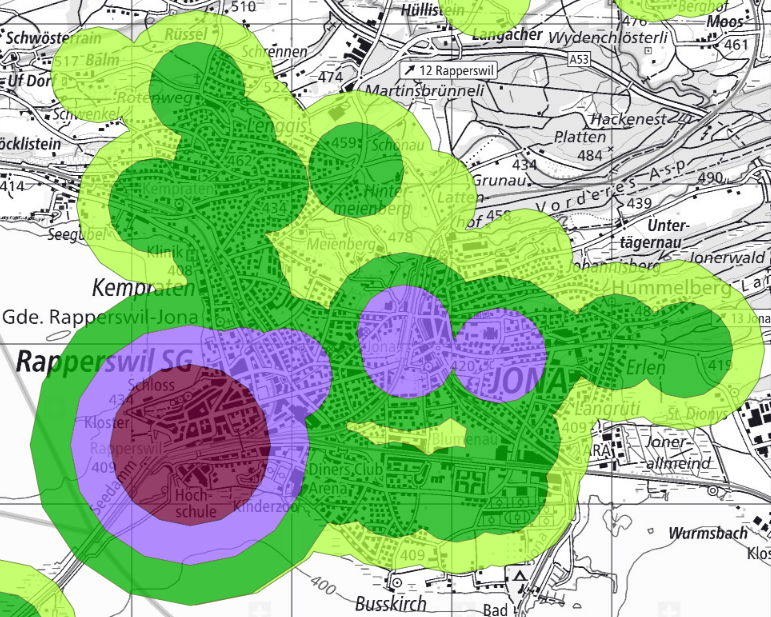
\includegraphics[width=0.50\linewidth]{start/img/air_line_ARE.png}
    \caption[Luftlinie bei Einzugsgebieten]{Luftlinie bei Einzugsgebieten~\cite{berechnung_are}}
    \label{fig:air_line_ARE}
\end{figure}

Der Wegführung wird in den aktuellen Lösungen keine und der Topografie nur wage Beachtung geschenkt.
So ist nicht klar, in welchem Mass eine anspruchsvollere Topografie zu Buche schlägt, denn eine Haltestelle in einem steilen Gebiet hat ein geringeres Einzugsgebiet als eine Haltestellen in einem flachen Gelände.

Erfahrungen aus der Praxis haben gezeigt, dass die bestehenden Lösungen einige Tücken in der Berechnung der Güteklassen aufweisen, welche zu einem falschen Schluss führen können.

\paragraph{Ziele, Vorgehen und Technologien}~\\
Im Kontext der Arbeit ÖV-Güteklassen 2018 wird in einem ersten Schritt eine neue Spezifikation entwickelt, welche auf dem Fundament der bestehenden Lösungen aufbaut, die Probleme und Learnings der kantonalen Anpassungen aufgreift und den aktuell technischen Möglichkeiten angleicht.

So soll unter anderem die genaue Wegführung beim Berechnung des Einzugsgebiet berücksichtigt und der Topografie Rechnung getragen werden.
Dies ist mit freiverfügbaren Kartedaten von OpenStreetMap (OSM) und dem   hoch aufgelöstem digitalen Terrainmodell (DTM) swissALTI$^{3D}$ von Swisstopo möglich.

Die theoretisch erarbeitete Spezifikation \emph{ÖV-Güteklassen 2018} wird direkt auf ihre Machbarkeit geprüft und als Generator umgesetzt, welche die Güteklassen berechnet.

Abgerundet wird Arbeit durch die Visualisierung der Güteklassen und einem direkten Vergleich der ÖV-Güteklassen basierend auf der neu erarbeitenden Spezifikation  und der bestehenden Lösung des Bundesamts für Raumentwicklung (ARE).

\paragraph{Ergebnisse}~\\
Durch die Erarbeitung der \emph{ÖV-Güteklassen 2018}-Spezifikation und der technischen Umsetzung dieser lassen sich Güteklassen generieren.
Diese sind in Abbildung \ref{fig:mntg_sum_resultat_webapp_uebersicht} ersichtlich.

Die Visualisierung bietet Raum- und Verkehrsplaner sowie Privatpersonen die Möglichkeit, Standorte auf die Qualität der ÖV-Erschliessung analysieren zu können, um so fundierte Entscheidungen in ihren Problemdomänen treffen zu können.

\begin{figure}[ht]
    \centering
    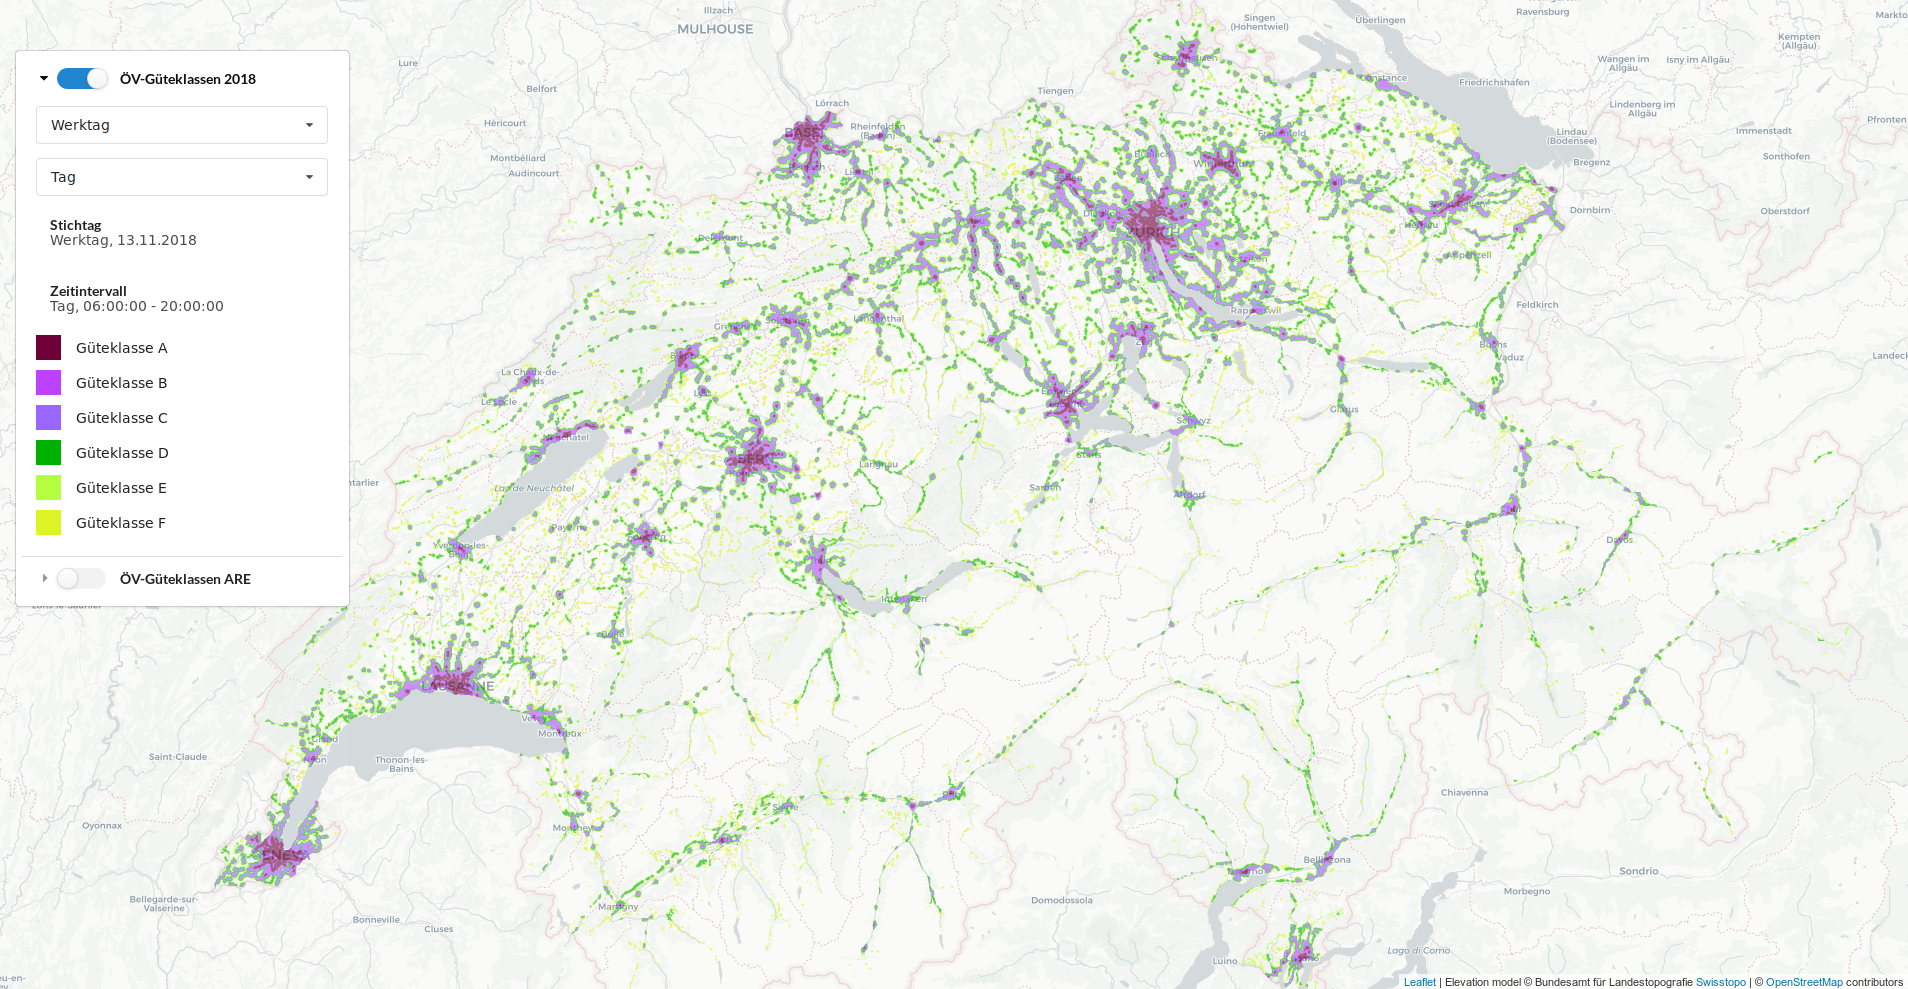
\includegraphics[width=1\linewidth]{technicalreport/img/resultat_oevgk18_uebersicht}
    \caption[Darstellung der berechneten ÖV-Güteklassen in der Web-Applikation]{Darstellung der berechneten ÖV-Güteklassen in der Web-Applikation}
    \label{fig:mntg_sum_resultat_webapp_uebersicht}
\end{figure}

Dabei wird unter anderem zusätzlich die Wegführung berücksichtigt, wie in Abbildung \ref{fig:vergleich_wegfuehrung} ersichtlich.
Die Topografie wird durch die Verwendung von Leistungskilometern in der Berechnung des Einzugsgebiet miteinbezogen.

\begin{figure}[ht]
    \centering
    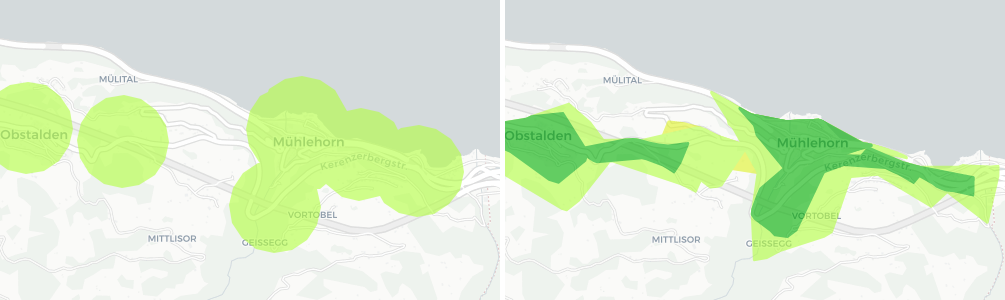
\includegraphics[width=0.8\linewidth]{start/img/vergleich_wegfuehrung}
    \caption[Vergleich zur Einfluss der Wegführung]{Vergleich zur Einfluss der Wegführung. Oben: ÖV-Güteklassen von \ac{ARE}. Unten: ÖV-Güteklassen 2018.}
    \label{fig:vergleich_wegfuehrung}
\end{figure}

\paragraph{Ausblick}~\\
In der vorliegenden Arbeit wurde beim Berechnen der Erreichbarkeit der Fokus auf eine route-basierte Methode, namentlich Isochronen, gelegt.
Ein weiterer spannender Ansatz, welcher in Betracht gezogen werden kann, ist ein grid- beziehungsweise raster-basierter Ansatz.
In Abbildung \ref{fig:mgmt_summary_grid_based_approach} wurde dieser Ansatz für die Berechnung der Reisezeit zu einer Haltestelle eines Fussgängers verwendet.
Dabei wird über ein Gebiet ein Raster gelegt, den Rastern eine Kategorie mit zugehörigen Kosten zugewiesen.
Bei den Kosten handelt es sich im abgebildeten Fall um die Überwindungsgeschwindigkeit des jeweiligen Rasters.
So erhält ein Raster mit einem Hinderniss beispielsweise die Geschwindigkeit 0 km/h und eine Grünfläche 2 km/h.
Dies hat unter anderem den Vorteil, dass man nicht direkt vom Routing-Netzwerk abhängig ist und auch offene Flächen wie Plätze und Grünflächen einbezogen werden.

Es lässt sich darüber streiten, ob alle Grünflächen von Fussgänger begehbar sind.
Ebenfalls lassen sich offene Fläche für die bestehende Lösung durch eine Vorverarbeitung des Routing-Netzwerk beispielsweise durch \emph{PlazaRoute}~\cite{plaza_route} ins Routing-Netzwerk integrieren.

\begin{figure}[ht]
    \centering
    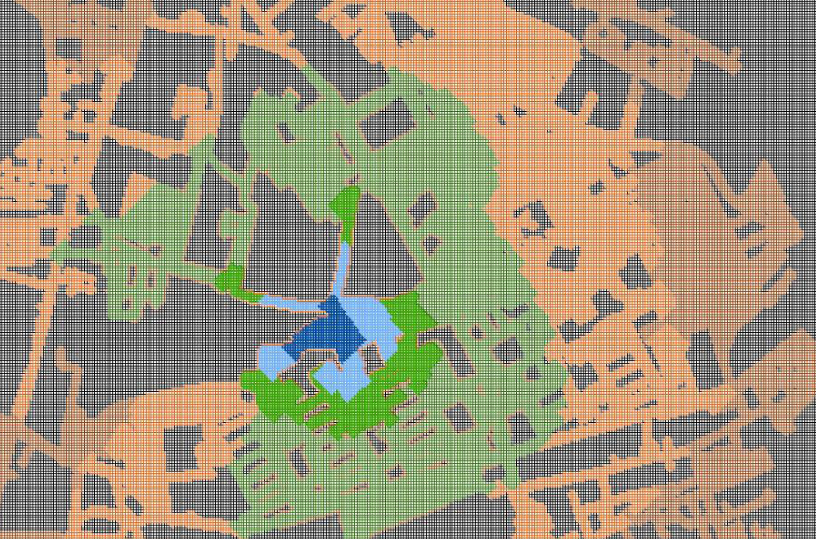
\includegraphics[width=0.6\linewidth]{start/img/grid_based_approach.png}
    \caption[Grid- beziehungsweise raster-basierter Ansatz]{Grid- beziehungsweise raster-basierter Ansatz~\cite{pedestrian_accessibility_planning}}
    \label{fig:mgmt_summary_grid_based_approach}
\end{figure}


\addcontentsline{toc}{chapter}{Inhaltsverzeichnis}
\tableofcontents

% not included in released version
% \addcontentsline{toc}{chapter}{Aufgabenstellung}
% \includepdf[pages=-, frame, scale=.9]{additionals/assignment.pdf}

% Summary index document for ...

\chapter{Technischer Bericht}
\label{Technischer Bericht}


\section{Einführung}
\label{Einführung}

%TODO

\subsection{Grundlagen und Begriffe}
\label{Einführung:Grundlagen und Begriffe}

%TODO

\subsection{Problemstellung und Vision}
\label{Einführung:Problemstellung und Vision}

%TODO

\subsection{Ziele und Unterziele}
\label{Einführung:Ziele und Unterziele}

%TODO

\subsubsection{Prototyp und Deliverables}
\label{Ziele und Unterziele:Prototyp und Deliverables}

%TODO

\subsection{Rahmenbedingungen, Umfeld, Definitionen und Abgrenzungen}
\label{Einführung:Rahmenbedingungen, Umfeld, Definitionen, Abgrenzungen}

%TODO

\subsection{Vorgehen und Aufbau der Arbeit}
\label{Einführung:Vorgehen und Aufbau der Arbeit}

%TODO



\section{Stand der Technik}
\label{Stand der Technik}

\subsection{Aktuelle Situation}
\label{Stand der Technik:Aktuelle Situation}

\subsubsection{Schweizer Norm 640 290}
\label{Aktuelle Situation:Schweizer Norm 640 290}

\acs{ÖV}-Güteklassen wurden erstmals mit der \ac{SN} 640 290~\cite{sn640290} des Vereins Schweizerischer Strassenfachleute (VSS) im Jahre 1993 für die Schweiz definiert.
Diese Norm enthält Richtwerte für die Bestimmung des Grenzbedarfs an Parkfeldern für Personenwagen und führte hierfür die Definition der \acs{ÖV}-Güteklassen ein.
Im Jahre 2006 wurde diese durch die \acs{SN} 640 281 abgelöst, welche nicht mehr auf die \acs{ÖV}-Güteklassen eingeht.
Es wurde seither keine allgemeingültige Definition verabschiedet.

Im Folgenden ist aufgeschlüsselt, was genau die \acs{SN} 640 290~\cite{sn640290} in Bezug auf \acs{ÖV}-Güteklassen definiert.

\paragraph{Definition ÖV-Güteklassen}~\\
\label{Schweizer Norm 640 290:Definition ÖV-Güteklassen}
Grundsätzlich definieren \acs{ÖV}-Güteklassen die Qualität der Erschliessung durch den öffentlichen Verkehr.
Diese Qualität wird durch die \nameref{Definition ÖV-Güteklassen:Bedienungsqualität der Haltestelle} und die \nameref{Definition ÖV-Güteklassen:Erreichbarkeit der Haltestelle} festgesetzt.
Beide Kriterien sind folgend definiert.
Anmerken muss man, dass zur besseren Verständlichkeit und Übersichtlichkeit zusätzliche Terminologie wie Verkehrsmittelkategorie eingeführt wird.

\subparagraph{Bedienungsqualität der Haltestelle}~\\
\label{Definition ÖV-Güteklassen:Bedienungsqualität der Haltestelle}
Die öffentlichen Verkehrsmittel werden zuerst in Verkehrsmittelkategorien eingeteilt:

\begin{itemize}[noitemsep]
    \item Verkehrsmittelkategorie 1
    \begin{itemize}
        \item Bahnknoten: mehrere Bahnlinien in unterschiedliche Richtungen
    \end{itemize}
    \item Verkehrsmittelkategorie 2
    \begin{itemize}
        \item Bahnlinie
    \end{itemize}
    \item Verkehrsmittelkategorie 3
    \begin{itemize}
        \item Tram, Trolleybus, Autobus, Regionalbus, Ortsbus mit gutem Anschluss an Bahnlinie
    \end{itemize}
    \item Verkehrsmittelkategorie 4
    \begin{itemize}
        \item Ortsbus, lokaler Kleinbus
    \end{itemize}
\end{itemize}

Die Verkehrsmittelkategorien werden dabei in die Gruppe A und B zusammengefasst, welche für die Berechnung des durchschnittlichen Kursintervalls berücksichtigt werden.
Dabei werden für die Intervallberechnung alle Verkehrsmittel der Verkehrsmittelkategorie in einer Gruppe berücksichtigt.
Daraus lassen sich die Haltestellenkategorien ermitteln (siehe Tabelle \ref{table:Ermittlung der Haltestellenkategorie (SN 640 290)}).


\begin{table}[ht]
    \begin{tabular}[c]{l | p{2.9cm} p{2.9cm} | p{2.9cm} p{2.9cm}}
        \toprule
        \textbf{Kursintervall}
                                & \multicolumn{4}{c}{\textbf{Verkehrsmittelkategorie}}\\
        \midrule
        \textbf{}
                                & \multicolumn{2}{c|}{\textbf{Gruppe A}}
                                & \multicolumn{2}{c}{\textbf{Gruppe B}}\\
        \textbf{}
                                & \textbf{1}
                                & \textbf{2}
                                & \textbf{3}
                                & \textbf{4}\\
        \textbf{< 5 min}
                                & I
                                & I
                                & II
                                & III\\
        \textbf{5 -- 9 min}
                                & I
                                & II
                                & III
                                & IV\\
        \textbf{10 -- 19 min}
                                & II
                                & III
                                & IV
                                & V\\
        \textbf{20 -- 39 min}
                                & III
                                & IV
                                & V
                                & V\\
        \textbf{40 -- 60 min}
                                & IV
                                & V
                                & V
                                & -\\
        \bottomrule
    \end{tabular}
    \caption{Ermittlung der Haltestellenkategorie (SN 640 290)}
    \label{table:Ermittlung der Haltestellenkategorie (SN 640 290)}
\end{table}

Das Kursintervall ist der durchschnittliche Abstand zwischen Ankunft beziehungsweise Abfahrt (pro Linie jeweils in der Hauptlastrichtung) aller Verkehrsmittel in der gleichen Gruppe zwischen 06:00 -- 20:00 Uhr jeweils von Montag bis Freitag.
Die Norm macht hier Ausnahmen bei Verdichtungen in Hauptverkehrszeiten, Linienüberlagerungen und reinen Arbeitsplatzgebieten mit stark verdichtetem Fahrplan während Pendlerzeiten.

\subparagraph{Erreichbarkeit der Haltestelle}~\\
\label{Definition ÖV-Güteklassen:Erreichbarkeit der Haltestelle}
Basierend auf den vorhin definierten Haltestellenkategorien (I bis V) kann die Erreichbarkeit pro Haltestellenkategorien definiert werden.
Die Distanzen sind Luftlinien, wobei ein mittlerer Umwegfaktor von 20 bis 30\% berücksichtigt wird.
Daraus lassen sich die \acs{ÖV}-Güteklassen ermitteln (siehe Tabelle \ref{table:Ermittlung Erreichbarkeit der Haltestelle (SN 640 290)})

\begin{table}[ht]
    \begin{tabular}[c]{l p{2.5cm} p{2.5cm} p{2.5cm} p{2.5cm}}
        \toprule
        \textbf{Haltestellenkategorie}
                                & \multicolumn{4}{c}{\textbf{Distanz zur Haltestelle}}\\
        \midrule
        \textbf{}
                                & \textbf{< 300 m}
                                & \textbf{300 -- 500 m}
                                & \textbf{501 -- 750 m}
                                & \textbf{751 -- 1000m}\\
        \textbf{I}
                                & Klasse A
                                & Klasse A
                                & Klasse B
                                & Klasse C\\
        \textbf{II}
                                & Klasse A
                                & Klasse B
                                & Klasse C
                                & Klasse D\\
        \textbf{III}
                                & Klasse B
                                & Klasse C
                                & Klasse D
                                & -\\
        \textbf{IV}
                                & Klasse C
                                & Klasse D
                                & -
                                & -\\
        \textbf{V}
                                & Klasse D
                                & -
                                & -
                                & -\\
        \bottomrule
    \end{tabular}
    \caption{Ermittlung der Erreichbarkeit der Haltestelle (SN 640 290)}
    \label{table:Ermittlung Erreichbarkeit der Haltestelle (SN 640 290)}
\end{table}

Der Topographie wird Rechnung getragen, indem man bei schwierigen Gegebenheiten die nächste Klasse wählt oder die Distanz vergrössert.

\subsection{Lösungsansätze}
\label{Stand der Technik:Lösungsansätze}
Basierend auf der bestehenden \nameref{Aktuelle Situation:Schweizer Norm 640 290} wurde im Jahre 2011 die Berechnungsmethodik des \ac{ARE} veröffentlicht, welche in einer Weisung des \acs{UVEK} vom 16.02.2015 als die Berechnugsmethodik definiert wird, welche bei der Beurteilung der Qualität der Erschliessung mit dem öffentlichen Verkehr verwendet werden soll.

In der Zwischenzeit haben einige Kantone Eigenlösungen entwickelt, welche Anpassungen an dieser Methodik und der \nameref{Aktuelle Situation:Schweizer Norm 640 290} vornehmen.
Folgend werden grob die Abweichungen zur Norm der Berechnungsmethodik ARE und zweier kantonaler Methodiken beschrieben, namentlich des Kanton Graubünden und Zürich.
Ebenfalls wird ein Blick auf eine österreichische Umsetzung der \acs{ÖV}-Güteklassen geworfen.
% TODO Grundlagenbericht erwähnen

Im Anschluss werden die Methodiken zusammen betrachtet, Schwachstellen eruiert und Verbesserungen vorgeschlagen.
Dieses Vorgehen hat das Ziel, Erfahrungen und etablierte Grundlagen in \gls{OeVGK18} im Kapitel \ref{Spezifikation OeVGK18} einfliessen zu lassen, um so eine allgemeine Akzeptanz erreichen zu können.

\subsubsection{Berechnungsmethodik ARE}
\label{Lösungsansätze:Berechnungsmethodik ARE}
Das Bundesamt für Raumentwicklung (ARE) entwickelt in ihrem Grundlagenbericht für die Beurteilung der Agglomerationsprogramme Verkehr und Siedlung~\cite{berechnung_are} eine Berechnungsmethodik der \acs{ÖV}-Güteklassen basierend auf der bestehende Norm (siehe Kapitel \ref{Aktuelle Situation:Schweizer Norm 640 290}).
Die entwickelte Berechnungsmethodik basiert auf den Fahrplandaten von HAFAS~\cite{sbb_hafas_spec}.
Dies hatte die Konsequenz, dass die Berechnungsmethodik so wie sie in der Norm festgelegt ist, angepasst werden musste.
Im Folgenden sind die Anpassungen aufgeführt.

\paragraph{Bedienungsqualität der Haltestelle}~\\
\label{Berechnungsmethodik ARE:Bedienungsqualität der Haltestelle}
Die Verkehrsmittel lassen sich aus dem elektronischen Fahrplan~\cite{sbb_hafas_spec} in der geforderten Tiefe nicht unterscheiden, wie es die Norm verlangt.
Dies hat die Konsequenz, dass die folgende Verkehrsmittel-Einteilung verwendet wird:

\begin{itemize}[noitemsep]
    \item Verkehrsmittelgruppe A
    \begin{itemize}
        \item Bahnknoten (mehrere Bahnlinien in verschiedenen Richtungen)
        \item Bahnlinien
    \end{itemize}
    \item Verkehrsmittelgruppe B
    \begin{itemize}
        \item Tram, Busse, Postautos, Rufbusse oder Schiffe
    \end{itemize}
    \item Verkehrsmittelgruppe C
    \begin{itemize}
        \item Seilbahnen
    \end{itemize}
\end{itemize}

Die Hauptlastrichtung kann aus den Fahrplandaten nicht extrahiert werden.
Somit werden alle Abfahrten zwischen 6.00 und 20.00 Uhr gezählt und anschliessend halbiert. Bei Endhaltestellen und Linien, welche nur in eine Richtung verlaufen, erfolgen Korrekturen.
Die genaue Art der Korrektur ist nicht weiter aufgeführt.
Als Stichtag für die Auswertung wird ein Werktag ausserhalb der Ferienzeit und der touristischen Hochsaison definiert.
Ebenfalls wir in reinen Arbeitsplatzgebieten mangels einheitlicher Definition keine Anpassung vorgenommen.
Verdichtungen in den Hauptverkehrszeiten sind in den gezählten Abfahrten inbegriffen.

\paragraph{Erreichbarkeit der Haltestelle}~\\
\label{Berechnungsmethodik ARE:Erreichbarkeit der Haltestelle}
Der Topographie wird keine Rechnung getragen, um eine landesweite Vergleichbarkeit sicherzustellen.

Die \acs{ÖV}-Güteklassen sind folgend zu interpretieren:

\begin{itemize}[noitemsep]
    \item Güteklasse A: Sehr gute Erschliessung
    \item Güteklasse B: Gute Erschliessung
    \item Güteklasse B: Mittelmässige Erschliessung
    \item Güteklasse D: Geringe Erschliessung
    \item Keine Güteklasse: Marginale oder keine \acs{ÖV}-Erschliessung
\end{itemize}

\subsubsection{Berechnungsmethodik Kanton Graubünden}
\label{Lösungsansätze:Berechnungsmethodik Kanton Graubünden}
Im technischen Bericht "`Definition \acs{ÖV}-Struktur / Erhebung  \acs{ÖV}-Güteklassen Kanton Graubünden"'~\cite{oev-guteklasse-gr} werden Anpassungen der in der Norm beschriebenen Berechnungsmethodik der \acs{ÖV}-Güteklassen an die speziellen Bedürfnisse des Kanton Graubündens, aber auch von allgemeiner Natur vorgenommen.
Anpassungen, welche spezielle Gegebenheiten des Kanton Graubündens betreffen, werden in der folgenden Zusammenstellung ausgeklammert, da sie sich für eine automatische Berechnung und für eine nationale Betrachtung nicht eignen.

\paragraph{Bedienungsqualität der Haltestelle}~\\
\label{Berechnungsmethodik Kanton Graubünden:Bedienungsqualität der Haltestelle}
Es werden zwei zusätzliche Haltestellenkategorien VI und VII (siehe Tabelle \ref{table:Ermittlung der Haltestellenkategorie (Kanton Graubünden)}) ergänzt und eine feinere Gliederung der Kursintervalls eingeführt.

Auf die Unterscheidung zwischen "`Tram, Trolleybus, Autobus, Regionalbus"' und "`Ortsbus, lokaler Kleinbus"' wird verzichtet und in der ersteren Kategorie zusammengefasst.
Ebenfalls werden Seilbahnen mit Erschliessungsfunktion wie Bushaltestellen behandelt.

\begin{table}[ht]
    \begin{tabular}[c]{l p{4.0cm} p{4.0cm} p{4.0cm}}
        \toprule
        \textbf{Kursintervall}
                                & \multicolumn{3}{c}{\textbf{Art des Verkehrsmittels}}\\
        \midrule
        \textbf{}
                                & \textbf{Bahnknoten}
                                & \textbf{Bahnlinie}
                                & \textbf{Tram/Bus}\\
        \textbf{< 5 min}
                                & I
                                & I
                                & II\\
        \cellcolor{red!25}\textbf{5 -- 10 min}
                                & I
                                & II
                                & III\\
        \cellcolor{red!25}\textbf{11 -- 19 min}
                                & II
                                & III
                                & IV\\
        \textbf{20 -- 39 min}
                                & III
                                & IV
                                & V\\
        \textbf{40 -- 60 min}
                                & IV
                                & V
                                & \cellcolor{red!25}VI\\
        \cellcolor{red!25}\textbf{> 60 min}
                                & -
                                & \cellcolor{red!25}VII
                                & \cellcolor{red!25}VII\\
        \bottomrule
    \end{tabular}
    \caption{Ermittlung der Haltestellenkategorie (Kanton Graubünden)}
    \label{table:Ermittlung der Haltestellenkategorie (Kanton Graubünden)}
\end{table}

Ebenfalls werden nun Bushaltestellen, die halbstündlich und stündlich bedient werden, nicht mehr gleich kategorisiert.
Auch werden Haltestellen erfasst, welche seltener als stündlich einen Anschluss haben.
Durch die feinere Gliederung des Kursintervalls erhält man eine bessere Güteklasse bei einem 10-Minuten-Takt im Vergleich mit einem 15-Minuten-Takt.

\paragraph{Erreichbarkeit der Haltestelle}~\\
\label{Berechnungsmethodik Kanton Graubünden:Erreichbarkeit der Haltestelle}
Die zusätzlichen Haltestellenkategorien (VI und VII) haben zur Folge, dass auch zwei zusätzliche Güteklassen E und F eingeführt werden (siehe Tabelle \ref{table:Ermittlung Erreichbarkeit der Haltestelle (Kanton Graubünden)}).

\begin{table}[ht]
    \begin{tabular}[c]{l p{2.5cm} p{2.5cm} p{2.5cm} p{2.5cm}}
        \toprule
        \textbf{Haltestellenkategorie}
                                & \multicolumn{4}{c}{\textbf{Distanz zur Haltestelle}}\\
        \midrule
        \textbf{}
                                & \textbf{< 300 m}
                                & \textbf{300 -- 500 m}
                                & \textbf{501 -- 750 m}
                                & \textbf{751 -- 1000m}\\
        \textbf{I}
                                & Klasse A
                                & Klasse A
                                & Klasse B
                                & Klasse C\\
        \textbf{II}
                                & Klasse A
                                & Klasse B
                                & Klasse C
                                & Klasse D\\
        \textbf{III}
                                & Klasse B
                                & Klasse C
                                & Klasse D
                                & -\\
        \textbf{IV}
                                & Klasse C
                                & Klasse D
                                & -
                                & -\\
        \textbf{V}
                                & Klasse D
                                & -
                                & -
                                & -\\
        \cellcolor{red!25}\textbf{VI}
                                & \cellcolor{red!25}Klasse E
                                & -
                                & -
                                & -\\
        \cellcolor{red!25}\textbf{VII}
                                & \cellcolor{red!25}Klasse F
                                & -
                                & -
                                & -\\                                
        \bottomrule
    \end{tabular}
    \caption{Ermittlung der Erreichbarkeit der Haltestelle (Kanton Graubünden)}
    \label{table:Ermittlung Erreichbarkeit der Haltestelle (Kanton Graubünden)}
\end{table}

Bushaltestellen haben eine maximale Erschliessungswirkung von 500 Meter, da grössere Distanzen von Passagieren als zu lange empfunden wird.
Somit werden nur Bahnknoten und Bahnlinien in den Kategorien > 500 Meter klassifiziert.
Die Topographie wird manuell berücksichtigt.

Hauptverkehrszeiten werden nicht gesondert gehandhabt.
Es zählt grundsätzlich das Angebot im gegebenen Zeitbereich.

Linien, welche grundsätzlich stündlich fahren, jedoch Taktlücken aufweisen um zu einen gewissen Zeitpunkt ein Angebot erfüllen zu können, werden nur in der Stundentakt-Gruppe klassifiziert, wenn sie nicht mehr als 2 Taktlücken aufweisen.

Es existieren Linienüberlagerungen mit einer ungleichen Verteilung.
So können zwei Linien stündlich verkehren und eine Haltestelle kurz nacheinander bedienen, welche dann als Halbstundentakt klassifiziert werden.
Der Passagier nimmt das Angebot aber als Stundentakt wahr.
Jedoch ist nicht weiter ersichtlich, wie das Problem behoben wird.

Die Bestimmung der Hauptlastrichtung erfolgt analog zur Berechnungsmethodik ARE.

% Brauchen uns Hinketakte zu interessieren und müssen wir das auflisten?

\subsubsection{Berechnungsmethodik Kanton Zürich}
\label{Lösungsansätze:Berechnungsmethodik Kanton Zürich}
Im Infoblatt "`ÖV-Güteklassen"'~\cite{oev-guteklassen-zh} wird beschrieben, wie der Kanton Zürich die kantonalen ÖV-Güteklassen mit den Fahrplandaten des Zürcher Verkehrsverbundes (ZVV), angelehnt an die Berechnungsmethodik \acs{ARE}, berechnet.

\paragraph{Bedienungsqualität der Haltestelle}~\\
\label{Berechnungsmethodik Kanton Zürich:Bedienungsqualität der Haltestelle}
Es werden nur Haltestellen berücksichtigt, die von Bahn, Tram und/oder Bus bedient werden.
Seilbahnen und Schiffe werden explizit ausgeklammert.
Somit ergibt sich folgende Kategorisierung:
\begin{itemize}
    \itemsep -1.5em
    \item Bahnknoten (Bahnstationen mit S-Bahnlinien in min. 6 Richtungen und/oder IR-Anschluss)
    \item Bahnlinien
    \item Tram
    \item Bus
\end{itemize}

Der Kursintervall wird auf 05:30 bis 22:30 Uhr festgelegt (unter der Woche).
Handelt es sich um Endhaltestellen oder Linien, welche nur in eine Richtung verkehren, werden alle Abfahrten gezählt.
Zusätzlich werden wie im Kanton Graubünden  Haltestellen mit einem Kursintervall von über 60 Minuten berücksichtigt (siehe Tabelle \ref{table:Ermittlung der Haltestellenkategorie (Kanton Zürich)}).

\begin{table}[ht]
    \begin{tabular}[c]{l p{2.9cm} p{2.8cm} p{2.8cm} p{2.8cm}}
        \toprule
        \textbf{Kursintervall}
                                & \multicolumn{4}{c}{\textbf{Art des Verkehrsmittels}}\\
        \midrule
        \textbf{}
                                & \textbf{Bahnknoten}
                                & \textbf{Bahnlinie}
                                & \textbf{Tram}
                                & \textbf{Bus}\\
        \textbf{< 5 min}
                                & I
                                & I
                                & II
                                & II\\
        \textbf{5 -- 9 min}
                                & I
                                & II
                                & III
                                & III\\
        \textbf{10 -- 19 min}
                                & II
                                & III
                                & IV
                                & IV\\
        \textbf{20 -- 39 min}
                                & III
                                & IV
                                & -
                                & V\\
        \textbf{40 -- 60 min}
                                & -
                                & V
                                & -
                                & VI\\
        \cellcolor{red!25}\textbf{> 60 min}
                                & -
                                & -
                                & -
                                & \cellcolor{red!25}VII\\
        \bottomrule
    \end{tabular}
    \caption{Ermittlung der Haltestellenkategorie (Kanton Zürich)}
    \label{table:Ermittlung der Haltestellenkategorie (Kanton Zürich)}
\end{table}


\paragraph{Erreichbarkeit der Haltestelle}~\\
\label{Berechnungsmethodik Kanton Zürich:Erreichbarkeit der Haltestelle}
Auch im Kanton Zürich werden durch den zusätzlich abgebildeten Kursintervall (> 60 Minuten) zwei neue Güteklassen E und F eingeführt (siehe Tabelle \ref{table:Ermittlung Erreichbarkeit der Haltestelle (Kanton Zürich)}).

\begin{table}[ht]
    \begin{tabular}[c]{l p{2.5cm} p{2.5cm} p{2.5cm} p{2.5cm}}
        \toprule
        \textbf{Haltestellenkategorie}
                                & \multicolumn{4}{c}{\textbf{Distanz zur Haltestelle}}\\
        \midrule
        \textbf{}
                                & \textbf{< 300 m}
                                & \textbf{300 -- 500 m}
                                & \textbf{501 -- 750 m}
                                & \textbf{751 -- 1000m}\\
        \textbf{I}
                                & Klasse A
                                & Klasse A
                                & Klasse B
                                & Klasse C\\
        \textbf{II}
                                & Klasse A
                                & Klasse B
                                & Klasse C
                                & Klasse D\\
        \textbf{III}
                                & Klasse B
                                & Klasse C
                                & Klasse D
                                & -\\
        \textbf{IV}
                                & Klasse C
                                & Klasse D
                                & \cellcolor{red!25}Klasse E
                                & -\\
        \textbf{V}
                                & Klasse D
                                & \cellcolor{red!25}Klasse E
                                & \cellcolor{red!25}Klasse E
                                & -\\
        \cellcolor{red!25}\textbf{VI}
                                & \cellcolor{red!25}Klasse E
                                & \cellcolor{red!25}Klasse E
                                & -
                                & -\\
        \cellcolor{red!25}\textbf{VII}
                                & \cellcolor{red!25}Klasse F
                                & \cellcolor{red!25}Klasse F
                                & -
                                & -\\                                
        \bottomrule
    \end{tabular}
    \caption{Ermittlung der Erreichbarkeit der Haltestelle (Kanton Zürich)}
    \label{table:Ermittlung Erreichbarkeit der Haltestelle (Kanton Zürich)}
\end{table}

Der Topographie wird keine Rechnung getragen, es wird strikt auf die Luftlinie gesetzt.
Sind Haltestellen nur durch Tram und/oder Bus erschlossen, werden analog zum Kanton Graubünden nur Distanzen bis zu 500 Meter berücksichtigt.
Die Erschliessung durch Bahnknoten und Bahnlinien wird bis 750 Meter mit den Güteklassen B -- E und bis 1000 Meter mit den Güteklassen C --D berücksichtigt.
Diese Entscheidungen basieren auf ÖV-Angebotsverordnungen.

\subsubsection{Berechnungsmethodik Österreich}
\label{Lösungsansätze:Berechnungsmethodik Österreich}

Im Artikel "`\acs{ÖV}-Güteklassen – ein Werkzeug zur Analyse der 
Versorgung eines Standortes mit ÖV"'~\cite{berechnung_oesterreich} ist die Umsetzung der Analyse der Versorgung eines Standortes mit öffentlichem Verkehr in Österreich beschrieben.

\paragraph{Bedienungsqualität der Haltestelle}~\\
\label{Berechnungsmethodik Österreich:Bedienungsqualität der Haltestelle}
Die Kursintervallberechnung erfolg analog zur \nameref{Lösungsansätze:Berechnungsmethodik ARE}.
Herauszuheben ist, dass zwei Stichtage definiert werden, ein gewöhnlicher Werktag und einen Tag, welcher ein besonders ungünstigen Verkehrstag wiederspiegelt.

Es wird keine grundsätzliche Unterscheidung zwischen Bahnknoten und Bahnlinien gezogen, sondern der Fernverkehr wird als das beste mögliche Verkehrsmittel angesehen.

\begin{table}[ht]
    \begin{tabular}[c]{l p{2.9cm} p{2.8cm} p{2.8cm} p{2.8cm}}
        \toprule
        \textbf{Kursintervall}
                                & \multicolumn{4}{c}{\textbf{Art des Verkehrsmittels}}\\
        \midrule
        \textbf{}
                                & \textbf{Fernverkehr REX}
                                & \textbf{S-Bahn, U-Bahn, \dots}
                                & \textbf{Strassenbahn, Metrobus, \dots}
                                & \textbf{Bus}\\
        \textbf{< 5 min}
                                & I
                                & I
                                & II
                                & \cellcolor{red!25}III\\
        \textbf{5 -- 9 min}
                                & I
                                & II
                                & III
                                & III\\
        \textbf{10 -- 19 min}
                                & II
                                & III
                                & IV
                                & IV\\
        \textbf{20 -- 39 min}
                                & III
                                & IV
                                & \cellcolor{red!25}V
                                & V\\
        \textbf{40 -- 60 min}
                                & \cellcolor{red!25}IV
                                & V
                                & \cellcolor{red!25}VI
                                & VI\\
        \cellcolor{red!25}\textbf{60 -- 120 min}
                                & \cellcolor{red!25}V
                                & \cellcolor{red!25}VI
                                & \cellcolor{red!25}VII
                                & \cellcolor{red!25}VII\\
        \cellcolor{red!25}\textbf{121 -- 210 min}
                                & -
                                & \cellcolor{red!25}VII
                                & \cellcolor{red!25}VIII
                                & \cellcolor{red!25}VIII\\
        \bottomrule
    \end{tabular}
    \caption{Ermittlung der Haltestellenkategorie (Österreich)}
    \label{table:Ermittlung der Haltestellenkategorie (Österreich)}
\end{table}

Es werden 3 weitere Haltestellenkategorien eingeführt und eine erweiterte Gliederung der Kursintervalle vorgenommen (siehe Tabelle \ref{table:Ermittlung der Haltestellenkategorie (Österreich)}).
So fliegen Haltestellen mit einem Intervall grösser 210 Minuten grundsätzlich bereits aus der Analyse.

\paragraph{Erreichbarkeit der Haltestelle}~\\
\label{Berechnungsmethodik Österreich:Erreichbarkeit der Haltestelle}
Durch die zusätzlichen Haltestellenkategorien und der feineren Kursintervallgliederung werden drei neue Güteklassen eingeführt, namentlich E, F und G.
Die Evaluierung der \acs{ÖV}-Güteklassen ist in Tabelle \ref{table:Ermittlung Erreichbarkeit der Haltestelle (Österreich)} ersichtlich.

Herauszuheben ist, dass die Wegführung berücksichtigt wird, was in den bisher analysierten Berechnungsmethodiken verwehrt blieb.
Von einer Haltestelle aus werden die zu Fuss bewältigbaren Wege ermittelt.

Zusätzlich werden die gebildeten \acs{ÖV}-Güteklasse-Polygone mit einem Raster, welches statistische Daten beinhaltet, verschnitten.
So kann man beispielsweise zusätzlich die Bevölkerungsdichte evaluieren.

\begin{table}[ht]
    \begin{tabular}[c]{l p{2.0cm} p{2.0cm} p{2.0cm} p{2.0cm} p{2.0cm}}
        \toprule
        \textbf{Haltestellenkategorie}
                                & \multicolumn{5}{c}{\textbf{Distanz zur Haltestelle}}\\
        \midrule
        \textbf{}
                                & \textbf{< 301 m}
                                & \textbf{301 -- 500 m}
                                & \textbf{501 -- 750 m}
                                & \textbf{751 -- 1000m}
                                & \textbf{1001 -- 1250m}\\
        \textbf{I}
                                & Klasse A
                                & Klasse A
                                & Klasse B
                                & Klasse C
                                & \cellcolor{red!25}Klasse D\\
        \textbf{II}
                                & Klasse A
                                & Klasse B
                                & Klasse C
                                & Klasse D
                                & \cellcolor{red!25}Klasse E\\
        \textbf{III}
                                & Klasse B
                                & Klasse C
                                & Klasse D
                                & \cellcolor{red!25}Klasse E
                                & \cellcolor{red!25}Klasse F\\
        \textbf{IV}
                                & Klasse C
                                & Klasse D
                                & \cellcolor{red!25}Klasse E
                                & \cellcolor{red!25}Klasse F
                                & \cellcolor{red!25}Klasse G\\
        \textbf{V}
                                & Klasse D
                                & \cellcolor{red!25}Klasse E
                                & \cellcolor{red!25}Klasse F
                                & \cellcolor{red!25}Klasse G
                                & \cellcolor{red!25}Klasse G\\
        \cellcolor{red!25}\textbf{VI}
                                & \cellcolor{red!25}Klasse E
                                & \cellcolor{red!25}Klasse F
                                & \cellcolor{red!25}Klasse G
                                & -
                                & -\\
        \cellcolor{red!25}\textbf{VII}
                                & \cellcolor{red!25}Klasse F
                                & \cellcolor{red!25}Klasse G
                                & \cellcolor{red!25}Klasse G
                                & -
                                & -\\
        \cellcolor{red!25}\textbf{VIII}
                                & \cellcolor{red!25}Klasse G
                                & \cellcolor{red!25}Klasse G
                                & -
                                & -
                                & -\\                          
        \bottomrule
    \end{tabular}
    \caption{Ermittlung der Erreichbarkeit der Haltestelle (Österreich)}
    \label{table:Ermittlung Erreichbarkeit der Haltestelle (Österreich)}
\end{table}

\subsection{Verbesserungsmöglichkeiten}
\label{Stand der Technik:Verbesserungsmöglichkeiten und Zusammenhang zu bestehenden Lösungen}
%TODO Abgrenzung zu Kapitel Problemstellung & Vision

Folgend werden identifizierte Schwachstellen der bestehenden Berechnungsmethodiken (siehe Kapitel \ref{Stand der Technik:Lösungsansätze}) aufgelistet und mögliche Optimierungen präsentiert.
Dabei behält man das Ziel der automatischen Berechnung hinter dem geistigen Auge.
Ob die definierten Kriterien mit der vorhandenen Datenbasis umsetzbar sind und ob diese für eine schweizweite Umsetzung tauglich ist, ist Bestandteil dieser Analyse.
Basierend auf diesen Verbesserungsmöglichkeiten, der \nameref{Lösungsansätze:Berechnungsmethodik ARE} und den Learnings der beiden kantonalen Berechnungsmethodiken wird im Kapitel \ref{Spezifikation OeVGK18} eine neue Methodik vorgeschlagen.

\subsubsection{Ermittlung der Erreichbarkeit der Haltestelle}
\label{Verbesserungsmöglichkeiten:Ermittlung der Erreichbarkeit der Haltestelle}

\paragraph{Problem}~\\
In allen Lösungen wird die Luftlinie als massgebende Bewertung der Erreichbarkeit einer Haltestelle genommen.
Dies berücksichtigt weder die zusätzliche Distanz durch verwinkelte Wege noch die Topographie.
Der Kanton Graubünden behebt diese Problematik mit manuellen Anpassungen.
Manuelle Eingriffe eigenen sich jedoch für eine automatisierte Lösung nicht.

\paragraph{Lösung}~\\
Um der Topographie und der Wegführung gerecht zu werden, wird einerseits der konkrete Weg entlang des Wege- und Strassennetzes für die Distanzberechnung berücksichtigt.
Auf der anderen Seite wird die Topographie durch die Berechnung von \gls{Leistungskilometer}n miteinbezogen.

\subsubsection{Wahl des Zeitintervalls}
\label{Verbesserungsmöglichkeiten:Wahl des Zeitintervalls}

\paragraph{Problem}~\\
Die Methodiken verwenden zur Berechnung des Kursintervalls grundsätzlich einen Werktag ausserhalb der Ferienzeit und der touristischen Hochsaison und einen Bereich, welcher den Pendlerverkehr zu den Randzeit berücksichtigt.
Der Kanton Zürich geht noch einen Schritt weiter und vergrössert ihren Einzugsbereich.
Die Kurse am Wochenende und in der Nacht werden grundsätzlich ausgeklammert.
Für Privatpersonen aber auch für Planer kann dieser Zeitraum relevant sein, um sich für einen Wohnort zu entscheiden oder um ein Angebot ausbauen zu können.

\paragraph{Lösung}~\\
Es werden drei Stichtage spezifiziert.
Zusätzlich zum Standardbereich, welcher den Pendlerverkehr berücksichtigt, wird der Verkehr ausserhalb des Pendlerverkehrs am Abend und am Wochenende berücksichtigt.
Die Gewichtung wird bei allen Zeitintervallen beibehalten, um einen quantitativen Vergleich zu ermöglichen.

\subsubsection{Kursintervall}
\label{Verbesserungsmöglichkeiten:Kursintervall}

\paragraph{Problem}~\\
Für die Bestimmung des Kursintervalls an einer Haltestelle werden in den bisherigen Berechnungsmethodiken in einem bestimmten Zeitintervall alle Abfahrten gezählt. Das Kursintervall wird bestimmt als Quotient aus Anzahl Abfahrten und der Dauer dieses Zeitintervalls, was den Mittelwert an Abfahrten pro Stunde ergibt.
Diese Methode berücksichtigt aber nicht die Verteilung der Abfahrten, was zu starken Verzerrungen führen kann.

Beachten wir als Beispiel eine fiktive Bushaltestelle, an der zu Beginn der Stunde gleich zwei Busse halten, dann aber für den Rest der Stunde kein einziger mehr.
Der Mittelwert an Abfahrten an dieser Haltestelle berechnet sich zu zwei Abfahrten pro Stunde, was ein Kursintervall von 30 Minuten ergibt.
Dies ist aber offensichtlich nicht ein realistischer Wert.
Aus Sicht eines Benutzers dieser Haltestelle handelt es sich eher um ein 60-minütiges Kursintervall.

\paragraph{Lösung}~\\
Für die Berechnung des Kursintervall wird statt der Anzahl Abfahrten die Wartezeit zwischen zwei Abfahrten als Grundlage verwendet.
Der Kursintervall $\tau$ einer Haltestelle wird definiert als das "`Doppelte der erwarteten Wartezeit auf die nächste Abfahrt [\ldots] bei zufälligem Zugang im Zeitintervall $I = [a,b)$"'.~\cite{visum_manual_formula}

Da die erwartete Ankunft bei zufälligem Zugang in der Mitte zwischen zwei regulären Abfahrten liegt, ergibt das Doppelte der erwarteten Wartezeit gerade das Kursintervall.

Wird das obige Beispiel mit diesem Ansatz erneut betrachtet, ergibt sich daraus ein Kursintervall von 58 Minuten (siehe Tabelle \ref{table:Vergleich der Kursintervallberechnung mit bisheriger und neuer Methodik}), was ein deutlich realistischeres Bild ergibt.

\begin{table}[ht]
    \centering
    \begin{tabular}[c]{l l l}
        \toprule
        \textbf{Berechnungsmethodik}
                                    & \textbf{Abfahrtszeiten}
                                    & \textbf{Berechneter Kursintervall}\\
        \midrule
        Bisherig
                                    & 09:01, 09:02, 10:01, 10:02, \dots
                                    & 30 Minuten\\
        Mittelwert aus Wartezeit    & 09:01, 09:02, 10:01, 10:02, \dots
                                    & 58 Minuten\\
        \bottomrule
    \end{tabular}
    \caption{Vergleich der Kursintervallberechnung mit bisheriger und neuer Methodik}
    \label{table:Vergleich der Kursintervallberechnung mit bisheriger und neuer Methodik}
\end{table}

\subsubsection{Bestimmung der Bahnknoten}
\label{Verbesserungsmöglichkeiten:Bestimmung der Bahnknoten}

\paragraph{Problem}~\\
Bei der Unterscheidung von Bahnknoten und Bahnlinien ist bei der Berechnungsmethodik vom \acs{ARE} lediglich spezifiziert, dass ein Bahnknoten Bahnlinien in mehrere Richtungen hat (siehe Kapitel \ref{Lösungsansätze:Berechnungsmethodik ARE}).
In den ÖV-Güteklassen des Kanton Zürichs werden Bahnknoten als "`Bahnstationen in mindestens 6 Richtungen und/oder nut IR-Anschluss"' (Kapitel \ref{Lösungsansätze:Berechnungsmethodik Kanton Zürich}) definiert.
Bei beiden Methodiken ist nicht klar, was unter einer Richtung genau zu verstehen ist.

Betrachtet man die resultierenden Daten der Berechnungsmethodik des \acs{ARE} ist ersichtlich, dass beispielsweise Genève-Aéroport als Bahnknoten identifiziert wird.
Diese Haltestelle bedient genau eine Richtung nach Genève.
Auf den ersten Blick könnte man annehmen, das die Identifizierung als Bahnknoten dadurch zustande kommt, weil die Haltestelle ein Flughafen erschliesst.
Dies wäre jedoch auf zwei Ebenen falsch, da in der Spezifikation dies nicht erwähnt wird und beispielsweise die Haltestelle Zürich Flughafen nicht als Bahnknoten identifiziert ist.
Anzumerken ist, dass die Haltestelle Zürich Flughafen 5 unterschiedliche Richtungen bedient.
Warum nun eine Haltestelle als Bahnknoten durchgeht oder eben nicht, entzieht sich unseren Kenntnissen.
Die fehlende Transparenz in der Bestimmung der Bahnknoten ist zu kritisieren.

\paragraph{Lösung}~\\
Für die Bestimmung von Bahnknoten werden von einer gegebenen Bahnstation aus diejenigen anderen Bahnstationen gezählt, die mit einem beliebigen Zug ohne Zwischenhalt erreicht werden können.
Konkret wird also für jeden (im definierten Zeitraum) an der Bahnstation haltenden Zug ermittelt, zu welcher Station er als nächstes fahren wird.
Die Anzahl Richtungen wird dann definiert als die Anzahl von verschiedenen Bahnstationen, die dadurch gezählt werden.



\section{Spezifikation OeVGK18}
\label{Spezifikation OeVGK18}

\subsection{Zusammenhang zur Berechnungsmethodik ARE}
\label{Spezifikation OeVGK18:Zusammenhang zur Berechnungsmethodik ARE}

In der Weisung des \acs{UVEK} vom 16.02.2015 ist festgehalten, dass für die Beurteilung der Qualität der Erschliessung mit dem öffentlichen Verkehr die \nameref{Lösungsansätze:Berechnungsmethodik ARE} verwendet wird~\cite{weisung_uvek}.
Dies ist der Grund warum im Folgenden der Bogen zu dieser Berechnungsmethodik geschlagen wird und die vorgeschlagenen Änderungen dieser Grundlagen gegenüber gestellt wird.
Die Berechnungsmethodik \acs{ARE} wird im Original~\cite{berechnung_are} zitiert und Anpassungen aus kantonalen Berechnungsmethodiken und eigene Verbesserungen werden, wo es Sinn macht, übernommen und gekennzeichnet.

\subsubsection{Art der Verkehrsmittel}
\label{Zusammenhang zur Berechnungsmethodik ARE:Art der Verkehrsmittel}

\begin{itquote}
Die Art der Verkehrsmittel, die an einer Haltestelle abfahren, wird wie folgt unterschieden:
\begin{itemize}[noitemsep]
    \item Verkehrsmittelgruppe A
    \begin{itemize}
        \item Bahnknoten (mehrere Bahnlinien in verschiedenen Richtungen)
        \item Bahnlinien
    \end{itemize}
    \item Verkehrsmittelgruppe B
    \begin{itemize}
        \item Tram, Busse, Postautos, Rufbusse oder Schiffe
    \end{itemize}
    \item Verkehrsmittelgruppe C
    \begin{itemize}
        \item Seilbahnen
    \end{itemize}
\end{itemize}
\end{itquote}

Die Verkehrsmittel werden weiterhin in drei Gruppen gehalten.
Aufgrund der neuartigen Berechnung des Kursintervalls sind Bahnknoten und Bahnlinie in separaten Gruppen eingeteilt und Seilbahnen werden mit den restlichen Verkehrsmittel zusammen betrachtet.

\begin{itemize}[noitemsep]
    \item Verkehrsmittelgruppe A
    \begin{itemize}
        \item Bahnknoten
    \end{itemize}
    \item Verkehrsmittelgruppe B
    \begin{itemize}
        \item Bahnlinie
    \end{itemize}
    \item Verkehrsmittelgruppe C
    \begin{itemize}
        \item Tram, Bus, Postauto, Rufbus, Schiff, Seilbahn
    \end{itemize}
\end{itemize}

Als Bahnknoten gelten analog zu Berechnungsmethodik des Kanton Zürich Bahnstationen, die entweder einen Anschluss an den nationalen oder internationalen Fernverkehr haben und/oder Bahnlinien in mindestens 6 Richtungen verkehren. 

\subsubsection{Kursintervall}
\label{Zusammenhang zur Berechnungsmethodik ARE:Kursintervall}

\begin{itquote}
Als Stichtag für die Auswertung wird ein Werktag ausserhalb der Ferienzeit und der touristischen Hochsaison definiert.
\end{itquote}

Die Einschränkung zur Wahl des Stichtags wird übernommen.
Jedoch werden 2 weitere Zeiträume definiert, einer für das Wochenende und jeweils einer für die Nacht.

\begin{itquote}
Zur Berechnung des Kursintervalls an einer Haltestelle werden aus dem elektronischen Fahrplan die Abfahrten auf allen Linien am Stichtag zwischen 6.00 und 20.00 Uhr gezählt.
Um die durchschnittliche Anzahl Abfahrten in eine Richtung zu ermitteln, wird die Anzahl Abfahrten halbiert.
Für Endhaltestellen sowie Haltestellen, die nur in einer Richtung befahren werden, erfolgen entsprechende Korrekturen.
Anschliessend wird das Kursintervall für die beiden Verkehrsmittelgruppen A und B separat berechnet (840 Minuten geteilt durch die korrigierte Anzahl Abfahrten).
\end{itquote}

Für die Kursintervallberechnung wird die statt der Anzahl Abfahrten die Wartezeit zwischen zwei Abfahrten als Grundlage verwendet.
Der Kursintervall $\tau$ einer Haltestelle wird definiert als das "`Doppelte der erwarteten Wartezeit auf die nächste Abfahrt [\ldots] bei zufälligem Zugang im Zeitintervall $I = [a,b)$"'~\cite{visum_manual_formula}.

\subsubsection{Haltestellenkategorie}
\label{Zusammenhang zur Berechnungsmethodik ARE:Haltestellenkategorie}

\begin{itquote}
Die Haltestellenkategorie wird nach folgender Tabelle ermittelt:
\begin{table}[ht]
    \centering
    \begin{itquote}
    \begin{tabular}[c]{l | p{2.3cm} p{2.3cm} | p{2.2cm} | p{2.2cm}}
        \toprule
        \textbf{Kursintervall}
                                & \multicolumn{4}{c}{\textbf{Verkehrsmittelgruppe}}\\
        \midrule
        \textbf{}
                                & \multicolumn{2}{c|}{\textbf{A}}
                                & \multicolumn{1}{c}{\textbf{B}}
                                & \multicolumn{1}{c}{\textbf{C}}\\
        \textbf{}
                                & \textbf{Bahnknoten}
                                & \textbf{Bahnlinien}
                                & \textbf{Trams, Busse, Postautos, Rufbusse und Schiffe}
                                & \textbf{Seilbahnen}\\
        \textbf{< 5 min}
                                & I
                                & I
                                & II
                                & III\\
        \textbf{5 -- 9 min}
                                & I
                                & II
                                & III
                                & IV\\
        \textbf{10 -- 19 min}
                                & II
                                & III
                                & IV
                                & V\\
        \textbf{20 -- 39 min}
                                & III
                                & IV
                                & V
                                & V\\
        \textbf{40 -- 60 min}
                                & IV
                                & V
                                & V
                                & V\\
        \bottomrule
    \end{tabular}
    \end{itquote}
\end{table}
\end{itquote}

Bei der Gliederung des Kursintervalls wird die Einteilung der Berechnungsmethodik des Kanton Graubünden übernommen.
Dies führt zu einer feineren und erweiterten Gliederung des Kursintervalls und zwei zusätzlichen Haltestellenkategorien VI und VII.

\subsubsection{Distanz zur Haltestelle}
\label{Zusammenhang zur Berechnungsmethodik ARE:Distanz zur Haltestelle}

\begin{itquote}
Für die Distanz zur Haltestelle wird die Luftliniendistanz verwendet, d.h. die ÖV-Güteklassen bilden konzentrische Kreise um die Haltestelle.
Die Radien der Kreise betragen 300 m, 500 m, 750 m und 1‘000 m.
\end{itquote}

Als Einteilung werden neu Gehminuten mit der Einstufung 5, 7.5, 10 und 15 Minuten verwendet.
Unter der Annahme, dass die Laufgeschwindigkeit $1.4 m/s$ beträgt, wird die massgebende Gehdauer mithilfe der Laufgeschwindigkeit und der Anzahl zurückzulegende \gls{Leistungskilometer} berechnet, welche die Topographie und die Wegführung berücksichtigt.

\subsubsection{ÖV-Güteklassen}
\label{Zusammenhang zur Berechnungsmethodik ARE:ÖV-Güteklassen}

\begin{itquote}
Die Güteklassen werden nach folgender Tabelle ermittelt:
\begin{table}[ht]
    \centering
    \begin{itquote}
    \begin{tabular}[c]{l p{2.2cm} p{2.2cm} p{2.2cm} p{2.2cm}}
        \toprule
        \textbf{Haltestellenkategorie}
                                & \multicolumn{4}{c}{\textbf{Distanz zur Haltestelle}}\\
        \midrule
        \textbf{}
                                & \textbf{< 300 m}
                                & \textbf{300 -- 500 m}
                                & \textbf{501 -- 750 m}
                                & \textbf{751 -- 1000m}\\
        \textbf{I}
                                & Klasse A
                                & Klasse A
                                & Klasse B
                                & Klasse C\\
        \textbf{II}
                                & Klasse A
                                & Klasse B
                                & Klasse C
                                & Klasse D\\
        \textbf{III}
                                & Klasse B
                                & Klasse C
                                & Klasse D
                                & keine\\
        \textbf{IV}
                                & Klasse C
                                & Klasse D
                                & keine
                                & keine\\
        \textbf{V}
                                & Klasse D
                                & keine
                                & keine
                                & keine\\
        \bottomrule
    \end{tabular}
    \end{itquote}
\end{table}
\end{itquote}

Durch die zusätzlichen Haltestellenkategorien VI und VII werden analog zur Berechnungsmethodik des Kanton Graubünden zwei weitere ÖV-Güteklassen E und F eingeführt.

\subsection{Berechnungsmethodik OeVGK18}
\label{Berechnungsmethodik OeVGK18}
Folgend wird die Berechnungsmethodik \gls{OeVGK18} detailliert beschrieben.
In Abbildung \ref{fig:Flow_OeVGK_Brechnung} ist zur Übersicht die Berechnung der \acs{ÖV}-Güteklassen schematisch dargestellt.
In einem ersten Schritt wird unter Berücksichtigung der Art der Verkehrsmittel (siehe Kapitel \ref{Berechnungsmethodik OeVGK18:Art der Verkehrsmittel}) und dem Kursintervall (siehe Kapitel \ref{Berechnungsmethodik OeVGK18:Kursintervall}) die Haltestellenkategorie (siehe Kapitel \ref{Berechnungsmethodik OeVGK18:Haltestellenkategorie}) eruiert.
Abschliessend werden mithilfe der Haltestellenkategorie und der Gehzeit zur Haltestelle (siehe Kapitel \ref{Berechnungsmethodik OeVGK18:Gehzeit zur Haltestelle}) die ÖV-Güteklassen (siehe Kapitel \ref{Berechnungsmethodik OeVGK18:ÖV-Güteklassen}) berechnet.

\begin{figure}[ht]
    \centering
    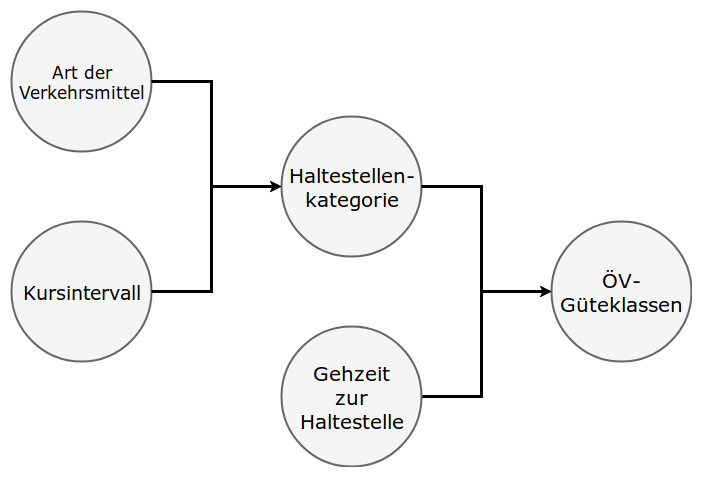
\includegraphics[width=0.7\linewidth]{technicalreport/img/Flow_OeVGK_Brechnung}
    \caption[Schema ÖV-Güteklassen Berechnung]{Schema ÖV-Güteklassen Berechnung}
    \label{fig:Flow_OeVGK_Brechnung}
\end{figure}

\subsubsection{Art der Verkehrsmittel}
\label{Berechnungsmethodik OeVGK18:Art der Verkehrsmittel}
Verkehrsmittel werden in folgende Verkehrsmittelgruppen eingeteilt:

\begin{itemize}[noitemsep]
    \item Verkehrsmittelgruppe A
    \begin{itemize}
        \item Bahnknoten
    \end{itemize}
    \item Verkehrsmittelgruppe B
    \begin{itemize}
        \item Bahnlinie
    \end{itemize}
    \item Verkehrsmittelgruppe C
    \begin{itemize}
        \item Tram, Bus, Postauto, Rufbus, Schiff, Seilbahn
    \end{itemize}
\end{itemize}

\paragraph{Bahnknoten}~\\
Bahnknoten sind Bahnstationen, die entweder einen Anschluss an den nationalen oder internationalen Fernverkehr haben und/oder Bahnlinien in mindestens 6 Richtungen verkehren.

Die Anzahl Richtungen einer Bahnstation wird gezählt als die Anzahl umliegender Bahnstationen, die mit einem beliebigen Zug innerhalb des definierten Zeitbereichs ohne Zwischenhalt erreicht werden können.

\paragraph{Schiffe und Seilbahnen}~\\
Schiffe und Seilbahnen werden nur berücksichtigt, wenn sie ein besiedeltes Wohngebiet erschliessen und nicht ausschliesslich für touristische Zwecke verwendet werden.


\subsubsection{Kursintervall}
\label{Berechnungsmethodik OeVGK18:Kursintervall}
Es sind 3 Stichtage mit jeweils zwei Zeitintervallen zu definieren, welche ausserhalb der Ferienzeit und der touristischen Hochsaison liegen.

\begin{table}[H]
    \centering
    \begin{tabular}[c]{l l}
        \toprule
        \textbf{Stichtag}
                                & \textbf{Zeitintervall}\\
        \midrule
        Werktag
                                & 06:00 -- 20:00 Uhr\\
        Werktag
                                & 20:00 -- 00:00 Uhr\\
        \midrule
        Samstag
                                & 06:00 -- 20:00 Uhr\\
        Samstag
                                & 01:00 -- 04:00 Uhr\\
        \midrule
        Sonntag
                                & 06:00 -- 20:00 Uhr\\
        Sonntag
                                & 01:00 -- 04:00 Uhr\\
        \bottomrule
    \end{tabular}
    \caption{Stichtag und Zeitintervall}
    \label{table:Stichtag und Zeitintervall}
\end{table}

Der Kursintervall $\tau$ einer Haltestelle wird definiert als das "`Doppelte der erwarteten Wartezeit auf die nächste Abfahrt [\ldots] bei zufälligem Zugang im Zeitintervall $I = [a,b)$"'~\cite{visum_manual_formula}.
Es werden nur Abfahrten betrachtet, die innerhalb des definiertem Zeitintervall an der Haltestelle abfahren.

Die Umsetzung dafür geschieht wie folgt:

\begin{tabbing}
Abfahrtszeitpunkte im Zeitintervall $I$: {\hskip 8em} \=    $x_{1 \ldots n}$      \\
Erste Abfahrt nach Zeitpunkt $b$ (nach Fahrplan): \>    $x'$                  \\
Fiktive Abfahrt nach $b$ bei zyklischer Fortsetzung: \> $x'' = x_1 + (b - a)$
\end{tabbing}

Für die Wartezeit am Zeitintervallende wird die Fahrt $x_{n+1} = min\{x', x''\}$ verwendet.

Kursintervall:
\[
    \tau^{a, b} = \frac{1}{b - a} \sum_{i=0}^n \Delta_i
\]

\begin{conditions}
    \Delta_i & $(x_{i+1} - x_i)^2$ {\hskip 2em} für $i \in \{1, \ldots, n - 1\}$ \\
    \Delta_0 & $(x_1 - a)^2$ \\
    \Delta_n & $(x_{n+1} - x_n)^2 - (x_{n+1} - b)^2$
\end{conditions}

\subsubsection{Haltestellenkategorie}
\label{Berechnungsmethodik OeVGK18:Haltestellenkategorie}
Die Haltestellenkategorie I bis VII wird mit folgender Tabelle eruiert:

\begin{table}[H]
    \begin{tabular}[c]{l p{4.0cm} p{4.0cm} p{4.0cm}}
        \toprule
        \textbf{Kursintervall [min]}
                                & \multicolumn{3}{c}{\textbf{Verkehrsmittelgruppe}}\\
        \midrule
        \textbf{}
                                & \textbf{A}
                                & \textbf{B}
                                & \textbf{C}\\
        \textbf{≤ 5}
                                & I
                                & I
                                & II\\
        \textbf{(5, 10]}
                                & I
                                & II
                                & III\\
        \textbf{(10, 20]}
                                & II
                                & III
                                & IV\\
        \textbf{(20, 40]}
                                & III
                                & IV
                                & V\\
        \textbf{(40, 60]}
                                & IV
                                & V
                                & VI\\
        \textbf{> 60}
                                & -
                                & VII
                                & VII\\
        \bottomrule
    \end{tabular}
    \caption{Haltestellenkategorie}
    \label{Haltestellenkategorie}
\end{table}

\subsubsection{Gehzeit zur Haltestelle}
\label{Berechnungsmethodik OeVGK18:Gehzeit zur Haltestelle}
Bei der Berechnung der Gehzeit zu einer Haltestelle ist eine Laufgeschwindigkeit von $1.4 m/s$ anzunehmen und die Strecke entlang des Wege- und Strassennetzes zu berücksichtigen, welche im folgenden als Horizontaldistanz bezeichnet wird.

Damit man der Topographie gerecht wird, ist als massgebende zu laufende Distanz Leistungsmeter zu verwenden:
\[
    x = 
\begin{cases}
    a + b/0.1 + c/0.15, & \text{wenn } c/d>0.22\\
    a + b/0.1,          & \text{sonst}
\end{cases}
\]
\begin{conditions}
    x   &   Leistungsmeter [m]\\
    a   &   Horizontaldistanz [m]\\
    b   &   positive Steigung in Höhenmeter [m]\\
    c   &   negative Steigung in Höhenmeter [m]\\
    d   &   Horizontaldistanz mit negativer Steigung [m]
\end{conditions}

Die Gehzeit $t$ zur Haltestelle ergibt sich nun aus:
\[ t = \frac{x}{1.4 m/s} \]


\subsubsection{ÖV-Güteklassen}
\label{Berechnungsmethodik OeVGK18:ÖV-Güteklassen}
Die Kombination aus Haltestellenkategorie und Gehzeit zur Haltestelle liefert folgende \acs{ÖV}-Güteklassen-Gruppierung:

\begin{table}[H]
    \begin{tabular}[c]{l p{2.6cm} p{2.6cm} p{2.6cm} p{2.6cm}}
        \toprule
        \textbf{Haltestellenkategorie}
                                & \multicolumn{4}{c}{\textbf{Gehzeit zur Haltestelle [s]}}\\
        \midrule
        \textbf{}
                                & \textbf{≤ 300}
                                & \textbf{(300, 450]}
                                & \textbf{(450, 600]}
                                & \textbf{(600, 900]}\\
        \textbf{I}
                                & Klasse A
                                & Klasse A
                                & Klasse B
                                & Klasse C\\
        \textbf{II}
                                & Klasse A
                                & Klasse B
                                & Klasse C
                                & Klasse D\\
        \textbf{III}
                                & Klasse B
                                & Klasse C
                                & Klasse D
                                & Klasse E\\
        \textbf{IV}
                                & Klasse C
                                & Klasse D
                                & Klasse E
                                & -\\
        \textbf{V}
                                & Klasse D
                                & Klasse E
                                & -
                                & -\\
        \textbf{VI}
                                & Klasse E
                                & -
                                & -
                                & -\\
        \textbf{VII}
                                & Klasse F
                                & -
                                & -
                                & -\\                                
        \bottomrule
    \end{tabular}
    \caption{ÖV-Güteklassen}
    \label{table:ÖV-Güteklassen}
\end{table}

Die Grenze wird bei einem Angebot schlechter als Stundentakt und einem Einzugsgebiet von 300 Sekunden gezogen, da man bei einer weiteren Betrachtung nicht mehr von einer Erschliessung reden kann und so auch nicht ausgewiesen werden soll.


% z.T. Wiederholung im Groben, z.T. Verweise auf Teil II-Kapitel

\section{Umsetzungskonzept}
\label{Umsetzungskonzept}

Die Arbeit wird in zwei von einander abhängigen Phasen umgesetzt.
Die erste Phase ist theoretisch gestaltet.
Dieser wird grosse Bedeutung beigemessen, da die zweite Phase auf den Ergebnissen dieser aufbaut.
So verfolgt die erste Phase das Ziel eine \acs{ÖV}-Güteklassen 2018 Spezifikation zu erstellen, mit dem Fokus schweizweit Akzeptanz zu erhalten.
Dies hat die Implikation, dass bestehende Lösungen, sprich die Spezifikation des \acl{ARE} und verschiedenen ausgewählten kantonale Ausführungen analysiert werden müssen, um so einen Konsens erreichen zu können.
Bewährtes und Akzeptiertes wird kritisch hinterfragt.
Dabei wird die Spezifikation so gestaltet, dass diese den aktuellen technischen Möglichkeiten gerecht wird.
Dies impliziert unter anderem die Verwendung eines Routing-Graphen für die Berechnung des Einzuggebiets und das Einbeziehen eines hoch aufgelösten digitalen Terrainmodells.
Dabei werden zusätzliche Fehler in den bisherigen Lösungen ausgemerzt.

In einer zweiten Phasen wird inkrementell die Spezifikation umgesetzt.
Dabei wird ein Generator entwickelt, welcher die \acs{ÖV}-Güteklassen aufgrund der in der ersten Phase erarbeiteten Spezifikation berechnet.
Parallel dazu wird eine Webapplikation mit zugehörigem Backend erarbeitet, welche die berechneten \acs{ÖV}-Güteklassen 2018 darstellt und visuell dem Platzhirsch (Spezifikation des \acl{ARE}) gegenüberstellt.
Diese Webapplikation verfolgt das Ziel, Verkehrs-, Raumplaner sowie Privatpersonen einen Einblick in die Qualität der ÖV-Erschliessung an einem Standort geben zu können.



\section{Resultate}
\label{Resultate}

In diesem Kapitel werden die Resultate der Arbeit präsentiert und mit den im Kapitel \ref{Stand der Technik:Aktuelle Situation} vorgestellten bestehenden Berechnungsmethoden verglichen.
Die technische Beschreibung zur Implementation befindet sich im Teil \ref{SW-Projektdokumentation} Kapitel \ref{Implementation}.

\subsection{Zielerreichung}
\label{Resultate:Zielerreichung}

In einer Evaluation (Teil \ref{Stand der Technik}) wurden bestehende Ansätze zur Berechnung von \gls{ÖV-Güteklassen} analysiert und verglichen.
Es zeigte sich, dass die Methoden auf einer alten Norm aufbauen, die von einigen Kantonen erweitert wurden.
Für die Berechnung der ganzen Schweiz gibt es aber keine Spezifikation, die moderne Analysen wie die Berücksichtigung des Strassennetzes vorsehen.

Unter Zuhilfenahme der verschiedenen Berechnungsmethodiken erstellten wir anschliessend eine eigene Spezifikation, die \gls{OeVGK18}.
Dabei haben wir neben einer genaueren Ermittlung der Erreichbarkeit (Kap. \ref{Verbesserungsmöglichkeiten:Ermittlung der Erreichbarkeit der Haltestelle}) und die Berücksichtigung des Terrains auch Punkte konkretisiert, die in bisherigen Methoden nicht genau spezifiziert sind, wie etwa die Berechnung des Kursintervalls (Kap. \ref{Verbesserungsmöglichkeiten:Kursintervall}) oder die Bestimmung von Bahnknoten (Kap. \ref{Verbesserungsmöglichkeiten:Bestimmung der Bahnknoten}).

In einem nächsten Schritt wurde die Berechnung anhand der \gls{OeVGK18}-Spezifikation umgesetzt und automatisiert.
So lassen sich die \gls{ÖV-Güteklassen} auch für nachfolgende Jahre neu berechnen.
Alle Parameter, die in der Spezifikation festgelegt wurden, sind in einer Konfigurationsdatei festgehalten und können beliebig verändert werden.
Dadurch kann die Implementation auch als Basis für Weiterentwicklungen der Berechnungsmethoden dienen.

\begin{landscape}
\begin{figure}[ht]
    \centering
    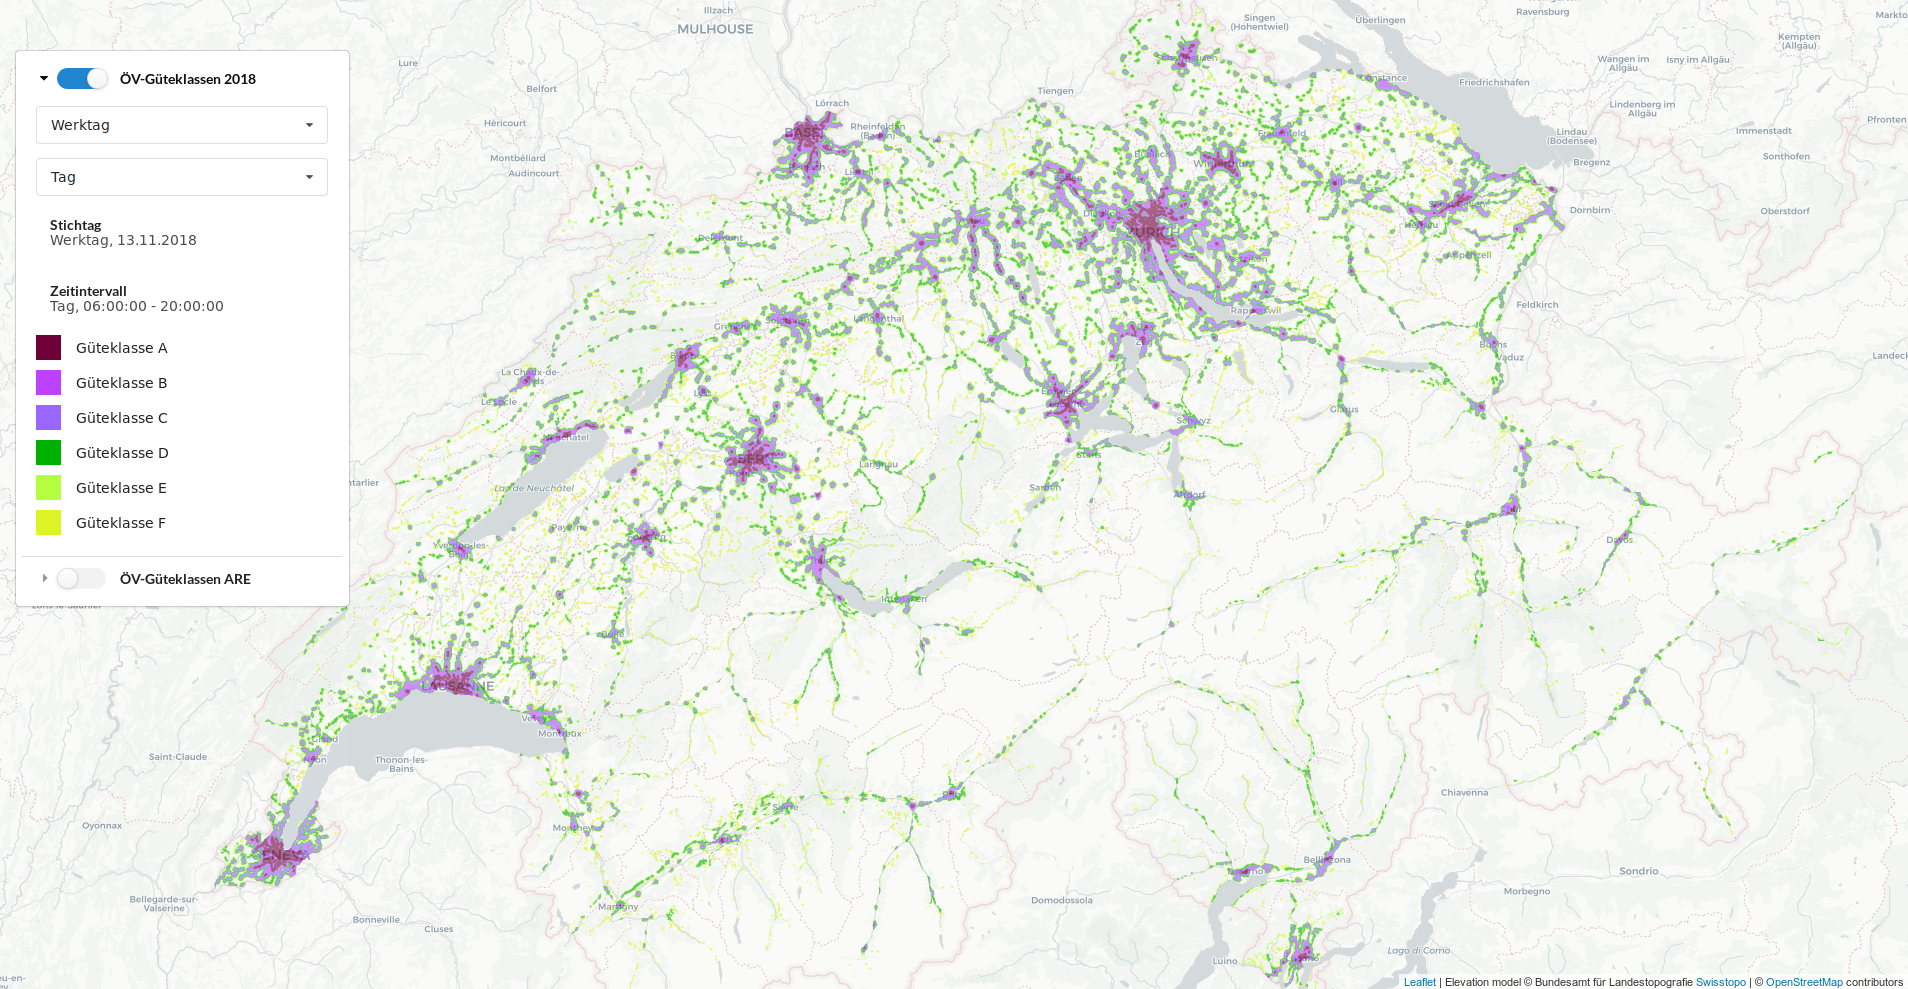
\includegraphics[width=1\linewidth]{technicalreport/img/resultat_oevgk18_uebersicht}
    \caption[Darstellung der berechneten ÖV-Güteklassen in der Web-Applikation]{Darstellung der berechneten ÖV-Güteklassen in der Web-Applikation}
    \label{fig:resultat_webapp_uebersicht}
\end{figure}
\end{landscape}

Zusätzlich zur automatisierten Berechnung wurde eine Web-Applikation entwickelt, die es ermöglicht, die berechneten \gls{ÖV-Güteklassen} im Browser darzustellen (siehe Abbildung \ref{fig:resultat_webapp_uebersicht}).
Ebenfalls wurden darin die bisherigen \gls{ÖV-Güteklassen} vom Bundesamt für Raumentwicklung (\acs{ARE}) integriert, was einen visuellen Vergleich der beiden Resultate erleichtert.

\subsection{Vergleich mit bisherigen ÖV-Güteklassen}
\label{Resultate:Vergleich mit bisherigen ÖV-Güteklassen}

Im Folgenden wird an einigen Beispielen gezeigt, wie die Resultate unserer Berechnung der \gls{OeVGK18} von bisherigen Methoden abweichen.
Als Vergleich werden dazu die \gls{ÖV-Güteklassen} von \ac{ARE} aus dem Jahre 2018~\cite{berechnung_are} verwendet.

\subsubsection{Einfluss der Wegführung}

\begin{figure}[ht]
    \centering
    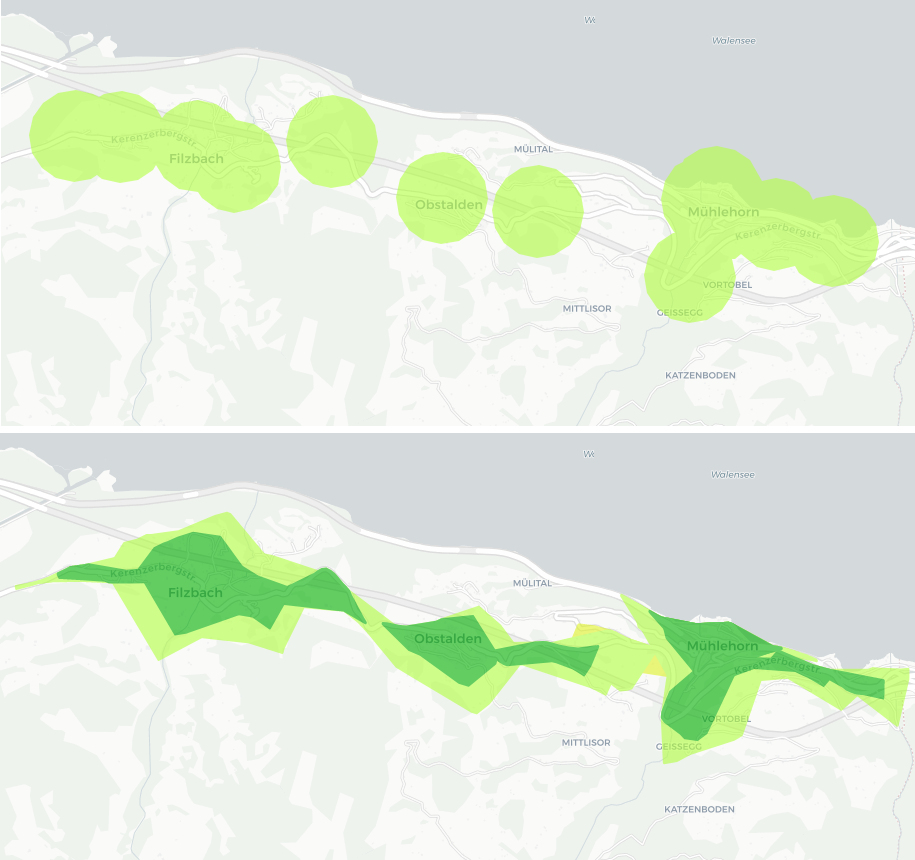
\includegraphics[width=0.8\linewidth]{technicalreport/img/vergleich_wegfuehrung}
    \caption[Vergleich zur Einfluss der Wegführung]{Vergleich zur Einfluss der Wegführung. Oben: ÖV-Güteklassen von \ac{ARE}. Unten: ÖV-Güteklassen 2018.}
    \label{fig:vergleich_wegfuehrung}
\end{figure}

Wie in \ref{Problemstellung:Luftlinie bei Einzugsgebieten} besprochen wird bei den bisherigen Ansätzen das Einzugsgebiet einer \gls{Haltestelle} mit einem Kreis, und somit als Luftlinie, beschrieben.
Mit \gls{OeVGK18} wird nun das Einzugsgebiet durch eine \gls{Isochrone} beschrieben.
Die Fläche zeigt das Einzugsgebiet, das von einem Fussgänger von der \gls{Haltestelle} aus in der definierten Zeit erreichbar ist.

Wie in Abbildung \ref{fig:vergleich_wegfuehrung} zu sehen ist, entstehen dadurch Geometrien, die dem Strassen- und Wegnetz folgen.
Dies ergibt einen realistischeren Eindruck über die effektiven Gebiete, die von einer \gls{Haltestelle} erschlossen werden.

Die Berücksichtigung der Wegführung ist im Direktvergleich in Abbildung \ref{fig:vergleich_wegfuehrung_are_isochrone} noch deutlicher sichtbar.

\begin{figure}[ht]
    \centering
    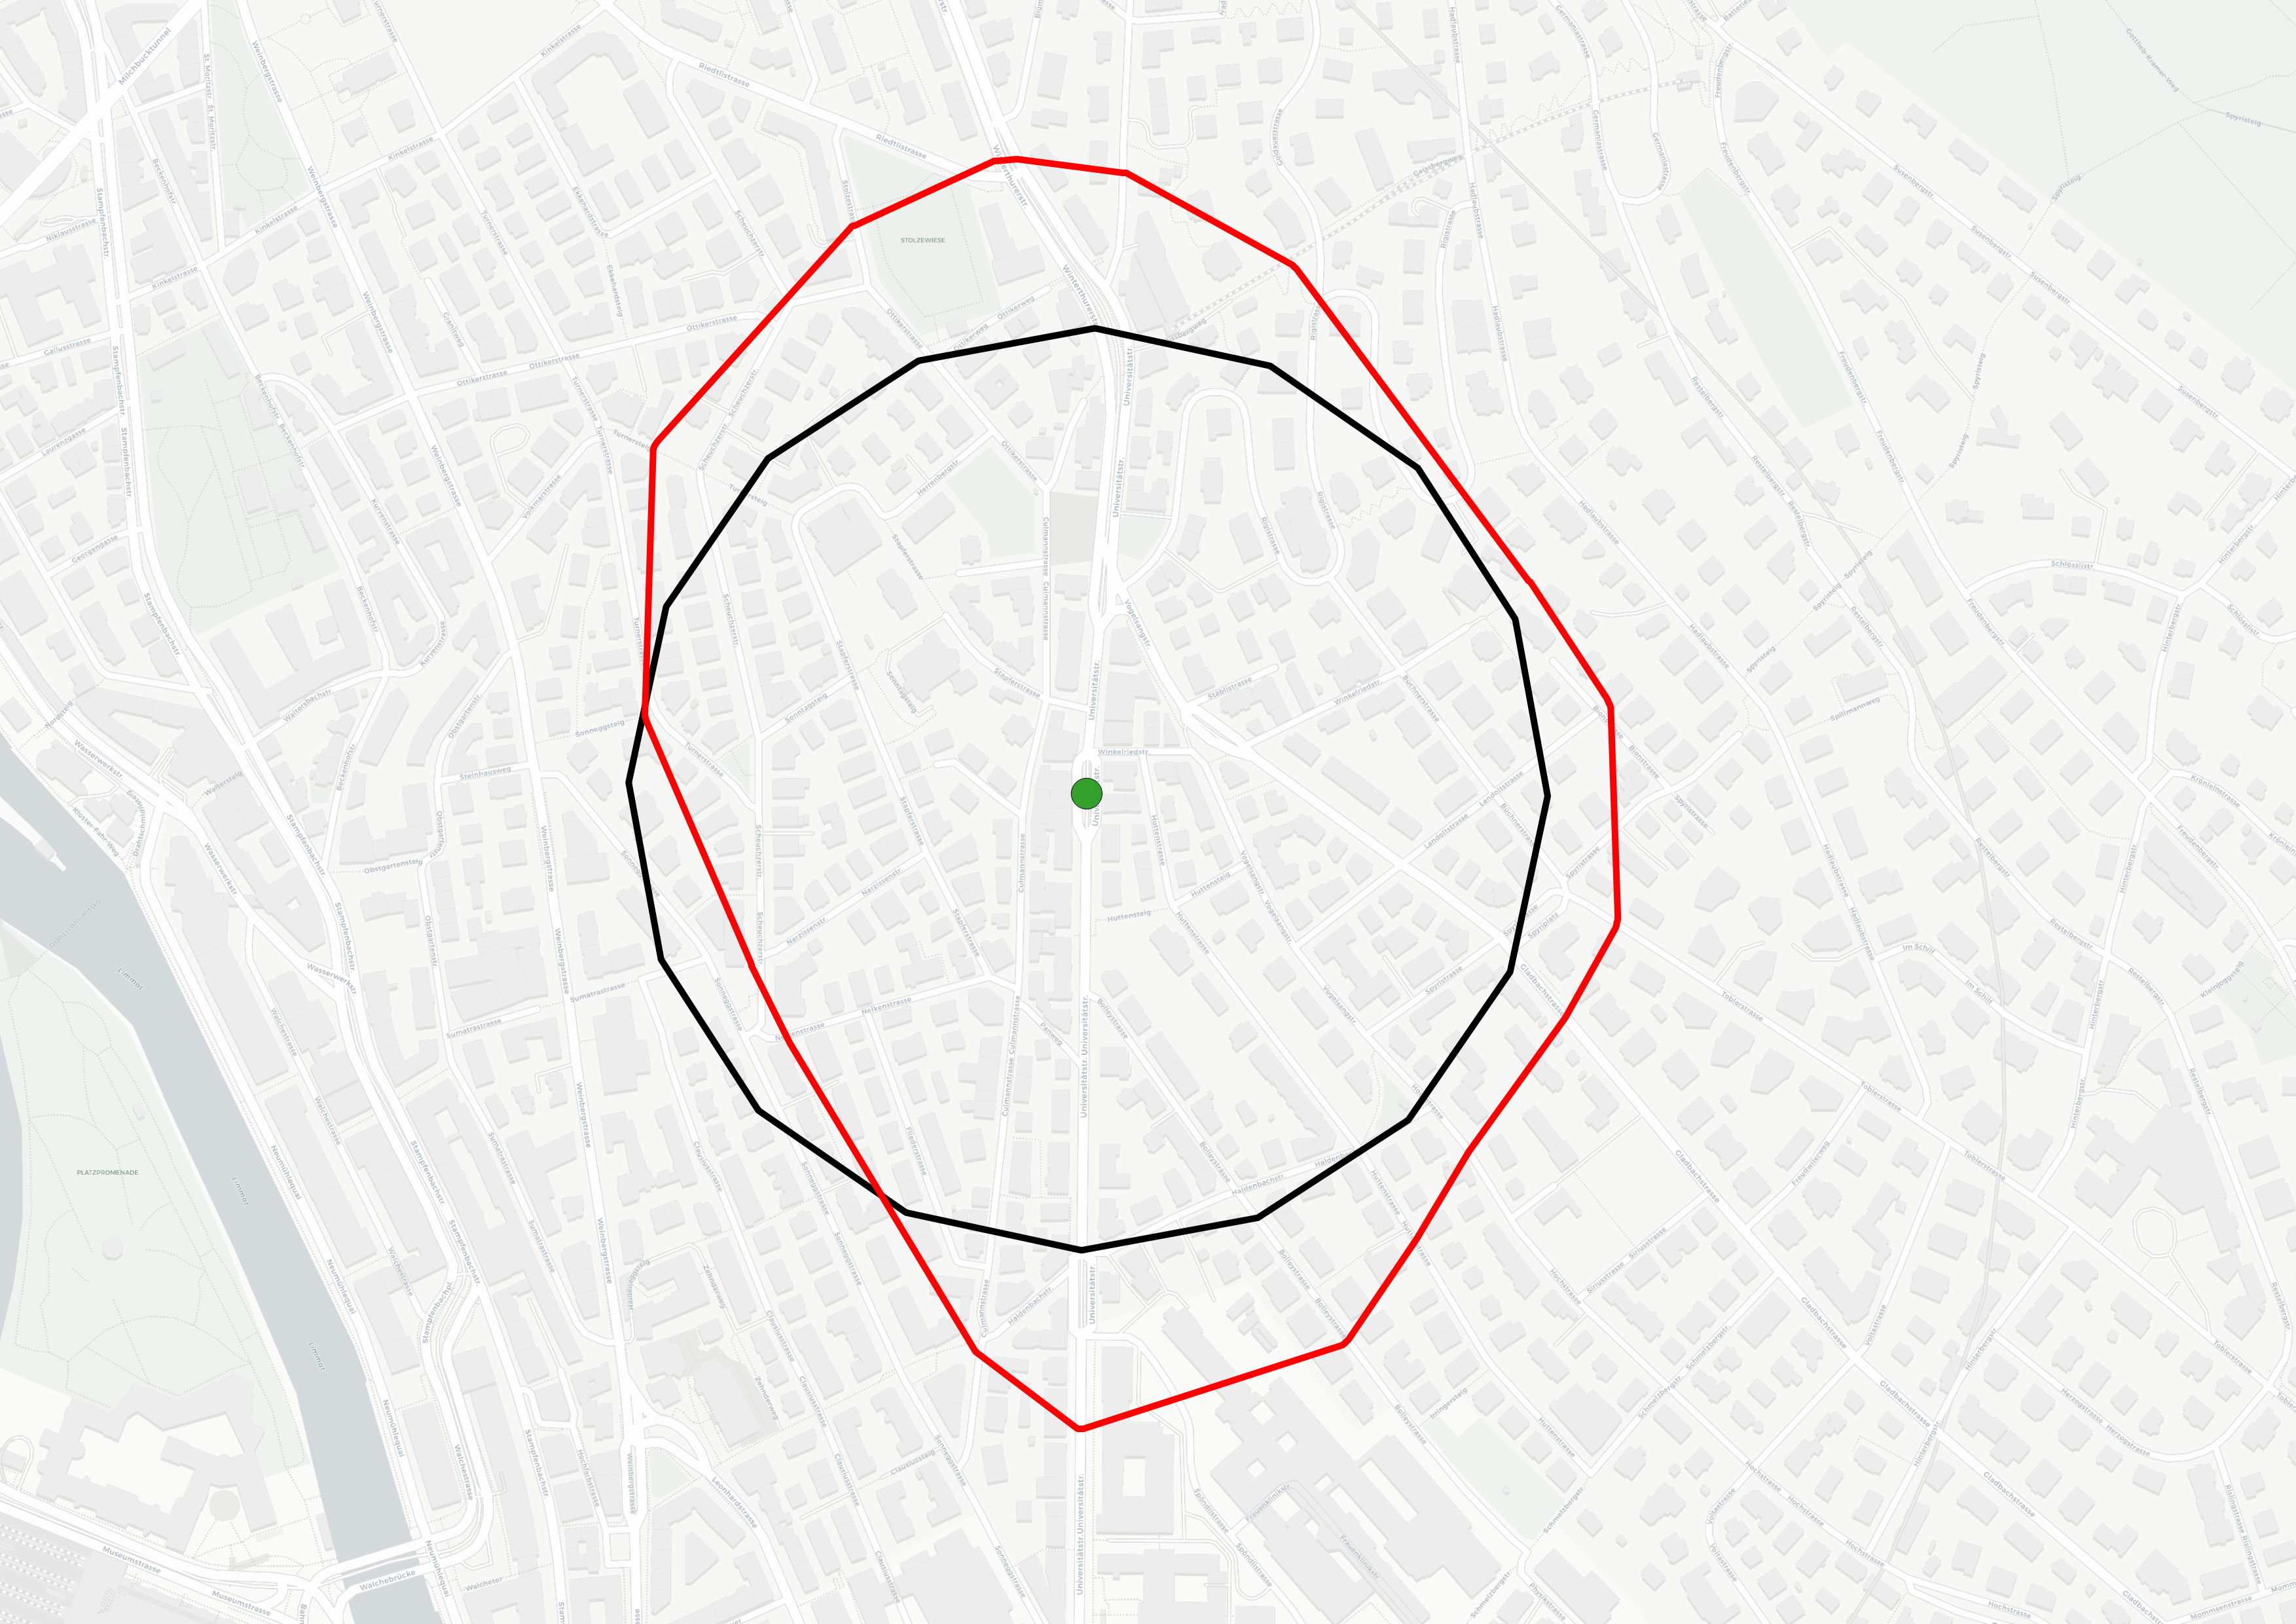
\includegraphics[width=0.8\linewidth]{technicalreport/img/vergleich_wegfuehrung_are_isochrone}
    \caption[Direktvergleich Einzugsgebiet ARE und Isochrone]{Direktvergleich Einzugsgebiet von ÖV-Güteklassen von \ac{ARE} (schwarz) und ÖV-Güteklassen 2018 (rot) ohne Berücksichtigung der Topographie; Haltestelle Zürich, Winkelriedstrasse}
    \label{fig:vergleich_wegfuehrung_are_isochrone}
\end{figure}

\subsubsection{Einfluss der Topographie}

Der Stand der Technik berücksichtigt die Topographie nicht konsequent.
Somit hat eine anspruchsvolle Topographie keinen Einfluss auf das Einzugsgebiet einer \gls{Haltestelle}.
Das sieht man gut, wenn man die ÖV-Güteklasse des \acl{ARE} in Abbildung \ref{fig:vergleich_wegfuehrung_are_isochrone} betrachtet.
Auf der gut sichbaren Strecke (Universitätsstrasse) werden im Durchmesser des schwarzen Kreises über eine Distanz von 300 Metern 9 Höhenmetern zurückgelegt.
Nach der Definition der Berechnung der \gls{Leistungskilometer}n (siehe Kapitel \ref{Berechnungsmethodik OeVGK18:Gehzeit zur Haltestelle}) sind das zu den 300 Metern zusätzliche 90 Leistungsmeter, welche zurückgelegt werden müssen.
Der Einfluss der Topographie ist nun im Direktvergleich in Abbildung \ref{fig:vergleich_wegfuehrung_isochrone_mit_ohne_topo} sichtbar.
Die \gls{Haltestelle} hat mit Einbezug der Topographie ein kleineres Einzugsgebiet.
Man sieht, dass sich dies gut im unteren Teil bemerktbar macht.
Die Strecke han von unten nach oben gesehen einen starken Anstieg, welcher ins Gewicht fällt.
Beachtet man die Fläche von oben nach unten, sieht man nur geringe Unterschiede, da das Gefälle den Grenzwert von 22\% nicht überschreitet.

\begin{figure}[ht]
    \centering
    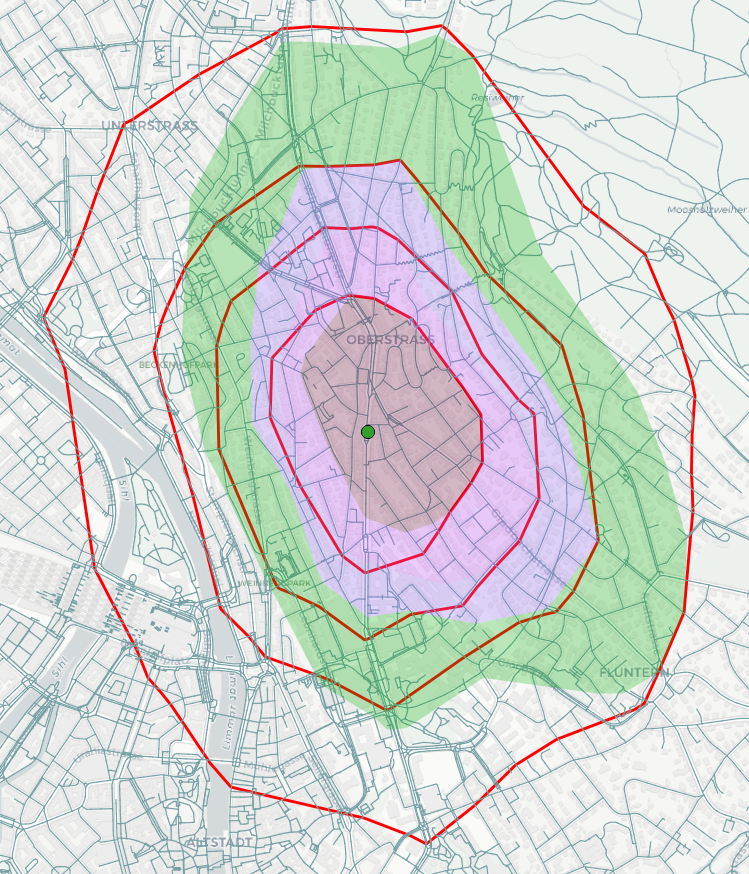
\includegraphics[width=0.8\linewidth]{technicalreport/img/vergleich_wegfuehrung_isochrone_mit_ohne_topo.png}
    \caption[Direktvergleich Einzugsgebiet Isochronen mit und ohne Topographie]{Direktvergleich Einzugsgebiet \glspl{Isochrone} mit (Fläche ausgefüllt) und ohne (rot) Berücksichtigung der Topographie; Haltestelle Zürich, Winkelriedstrasse}
    \label{fig:vergleich_wegfuehrung_isochrone_mit_ohne_topo}
\end{figure}


\subsubsection{Verbesserte Berechnung des Kursintervalls}

Der Unterschied in der Berechnung des Kursintervalls ist gut sichtbar, wenn man die \gls{Haltestelle} "`Aarau, Buchenhof"' betrachtet.
Damit wir die Berechnungsmethodiken \gls{OeVGK18} und \gls{OeVGKARE} vergleichen können, nehmen wir für die Auswertung von \gls{OeVGK18} den Stichtag 21.03.2018. Die Fahrplandaten des \gls{OeVGKARE} stammen vom 21.03.2017.
Dieser Vergleich ist in diesem Zusammenhang zulässig, da beide einen Werktag repräsentieren und keine Änderung im Fahrplan erkannt wurde.
Ebenfalls sieht man für diese \gls{Haltestelle} die Korrektur, welche das \ac{ARE} für Verbindungen vornimmt, welche nur in eine Richtung befahren werden.
So wird die Anzahl Verbindungen in diesem Fall verdoppelt, um sie anschliessend bei der Berechnung wieder zu halbieren.

An diesem Tag werden im Intervall 06:00 bis 20:00 Uhr 56 Fahrten an dieser \gls{Haltestelle} registriert.
Folgt man der Berechnungslogik des Bundesamts für Raumentwicklung, erfolgt daraus folgender Intervall:
$ 840 / ((56 * 2) / 2) = 15 \text{min}$

Betrachtet man nun einen Auszug der Abfahrten in Tabelle \ref{table:Abfahrtszeiten Aarau, Buchenhof}, sieht man, dass beide Buslinien 4 Minuten versetzt alle 30 Minuten verkehren.
Die Aussage, dass man an dieser \gls{Haltestelle} einen 15-Minuten-Takt hat, ist somit nicht ganz korrekt.
Kommt man um 06:10 Uhr an die \gls{Haltestelle}, wartet man 23 Minuten auf die nächste Verbindung.

\begin{table}[H]
    \centering
    \begin{tabular}[c]{l l}
        \toprule
        \textbf{Abfahrtszeit}   & \textbf{Bus-Nr}\\
        \midrule
        06:03                   & 7\\
        06:07                   & 5\\
        06:33                   & 7\\
        06:37                   & 5\\
        07:03                   & 7\\
        07:07                   & 5\\
        07:33                   & 7\\
        07:37                   & 5\\
        \dots                   & \dots\\
        \bottomrule
    \end{tabular}
    \caption{Abfahrtszeiten Bus 5 und 7, Haltestelle Aarau, Buchenhof}
    \label{table:Abfahrtszeiten Aarau, Buchenhof}
\end{table}

Die neue Intervall-Berechnung gemäss Kapitel \ref{Berechnungsmethodik OeVGK18:Kursintervall} ergibt nun für die gleiche \gls{Haltestelle} den Intervall 23.1 Minuten.
Der Unterschied macht sich in der Bestimmung der Haltestellenkategorie bemerkbar.
Da es sich bei dieser \gls{Haltestelle} um eine Busstation handelt, fällt man nach der \gls{OeVGK18}-Spezifikation von der Haltestellekategorie IV (\gls{OeVGKARE}) in die Kategorie V.

Abschliessend kann man sagen, dass 23.1 Minuten eine bessere Annäherung an den eigentlichen Kursintervall als die 15 Minuten, die vom \acs{ARE} berechnet wurde, ist.
Dadurch wird das wahrgenommene Angebot an der \gls{Haltestelle} besser wiederspiegelt.

\subsubsection{Verbesserte Ermittlung von Bahnknoten}
Bei der Ermittlung der Bahnknoten werden nur \glspl{Haltestelle} berücksichtigt, welche Verbindungen in 6 verschiedene Richtungen oder Zugang zu einer Fernverkehrsverbindung haben.
Aufgrund der Daten des \acl{ARE} nehmen wir an, dass bei der Berechnung der \gls{OeVGKARE} nur \glspl{Haltestelle} als Bahnknoten identifiziert werden, welche mindestens drei verschiedene Richtungen bedienen.
Diese Annahme kommt zustande, wenn man für die Bahnknoten des \gls{OeVGKARE} die Anzahl verschiedenen Richtungen mit unserer Implementation eruiert.
Dabei gibt es mit "`Genève-Aéroport"' einen Ausreiser, welcher nur eine Richtung anbietet.
Die Problematik ist in Kapitel \ref{Verbesserungsmöglichkeiten:Bestimmung der Bahnknoten} beschrieben.

Ein direkter Vergleich ist in Tabelle \ref{table:Vergleich Anzahl Bahnknoten} ersichtlich.

\begin{table}[H]
    \centering
    \begin{tabular}[c]{l l l}
        \toprule
        \textbf{}
                                & \textbf{\gls{OeVGKARE}}
                                & \textbf{\gls{OeVGK18}}\\
        \midrule
        \textbf{Anzahl Bahnknoten}
                                & 150
                                & 106\\
        \bottomrule
    \end{tabular}
    \caption{Vergleich Anzahl Bahnknoten}
    \label{table:Vergleich Anzahl Bahnknoten}
\end{table}

Da wir mindestens doppelt so viele verschiedene Richtungen wie \gls{OeVGKARE} verlangen, schränken wir so die Identifikation als Bahnknoten ein, was sich in der Anzahl identifizierter Bahnknoten bemerkbar macht.

\begin{table}[H]
    \centering
    \begin{tabular}[c]{l l l}
        \toprule
        \textbf{}
                                            & \textbf{Anzahl Bahnknoten}\\
        \midrule
        \textbf{\gls{OeVGKARE} $\cap$ \gls{OeVGK18}}       & 92\\
        \textbf{\gls{OeVGKARE} $\setminus$ \gls{OeVGK18}}  & 58\\
        \textbf{\gls{OeVGK18} $\setminus$ \gls{OeVGKARE}}  & 14\\
        \bottomrule
    \end{tabular}
    \caption{Unterschiede in der Identifikation der Bahnknoten}
    \label{table:Unterschiede in der Identifikation der Bahnknoten}
\end{table}

Dass durch die höhere Anzahl verlangter verschiedener Richtungen eine kleinere Menge als Bahnknoten identifizierte \glspl{Haltestelle} resultiert, scheint logisch.
Tabelle \ref{table:Unterschiede in der Identifikation der Bahnknoten} nimmt die Unterschiede in den resultierenden Bahnknoten unter die Lupe.
Überraschend ist, dass die Bahnknoten, welche durch \gls{OeVGK18} identifiziert werden, nicht komplett in \gls{OeVGKARE} vorkommen.
Es handelt sich um 14 \glspl{Haltestelle}, welche \gls{OeVGK18} im Unterschied zu \gls{OeVGKARE} als Bahnknoten bestimmt werden.
Dabei handelt es sich unter diesen um 2 \glspl{Haltestelle}, welche eine Fernverkehrsverbindung haben und so als Bahnknoten gezählt werden.
Warum die restlichen 12 \glspl{Haltestelle} nicht ebenfalls als Bahnknoten identifiziert sind, entzieht sich unseren Kenntnissen.
Darunter fällt beispielsweise die Haltestelle Flüelen mit 9 verschiedenen Richtungen.

\subsection{Vergleich ÖV-Güteklassen mit unterschiedlichen Stichtagen und Zeitintervallen}
\label{Resultate:Vergleich ÖV-Güteklassen mit unterschiedlichen Stichtagen und Zeitintervallen}

Bisher hat man sich auf einen Stichtag ausserhalb der touristischen Hochsaison beschränkt, um so ein allgemeingültiges Resultat zu erhalten.
Dadurch schränkt man die Auswertungsmöglichkeiten stark ein, da die Qualität der \acs{ÖV}-Erschliessung beispielsweise an einem Wochenende oder am Abend/in der Nacht genauso interessant auszuwerten ist wie tagsüber.
Durch die Konfigurationsmöglichkeit des "`\gls{ÖV-Güteklassen} 2018 Generators"' ist es eine Leichtigkeit, in einem Schritt die \gls{ÖV-Güteklassen} für unterschiedliche Stichtage und Zeitintervalle zu berechnen.

\begin{figure}[ht]
    \centering
    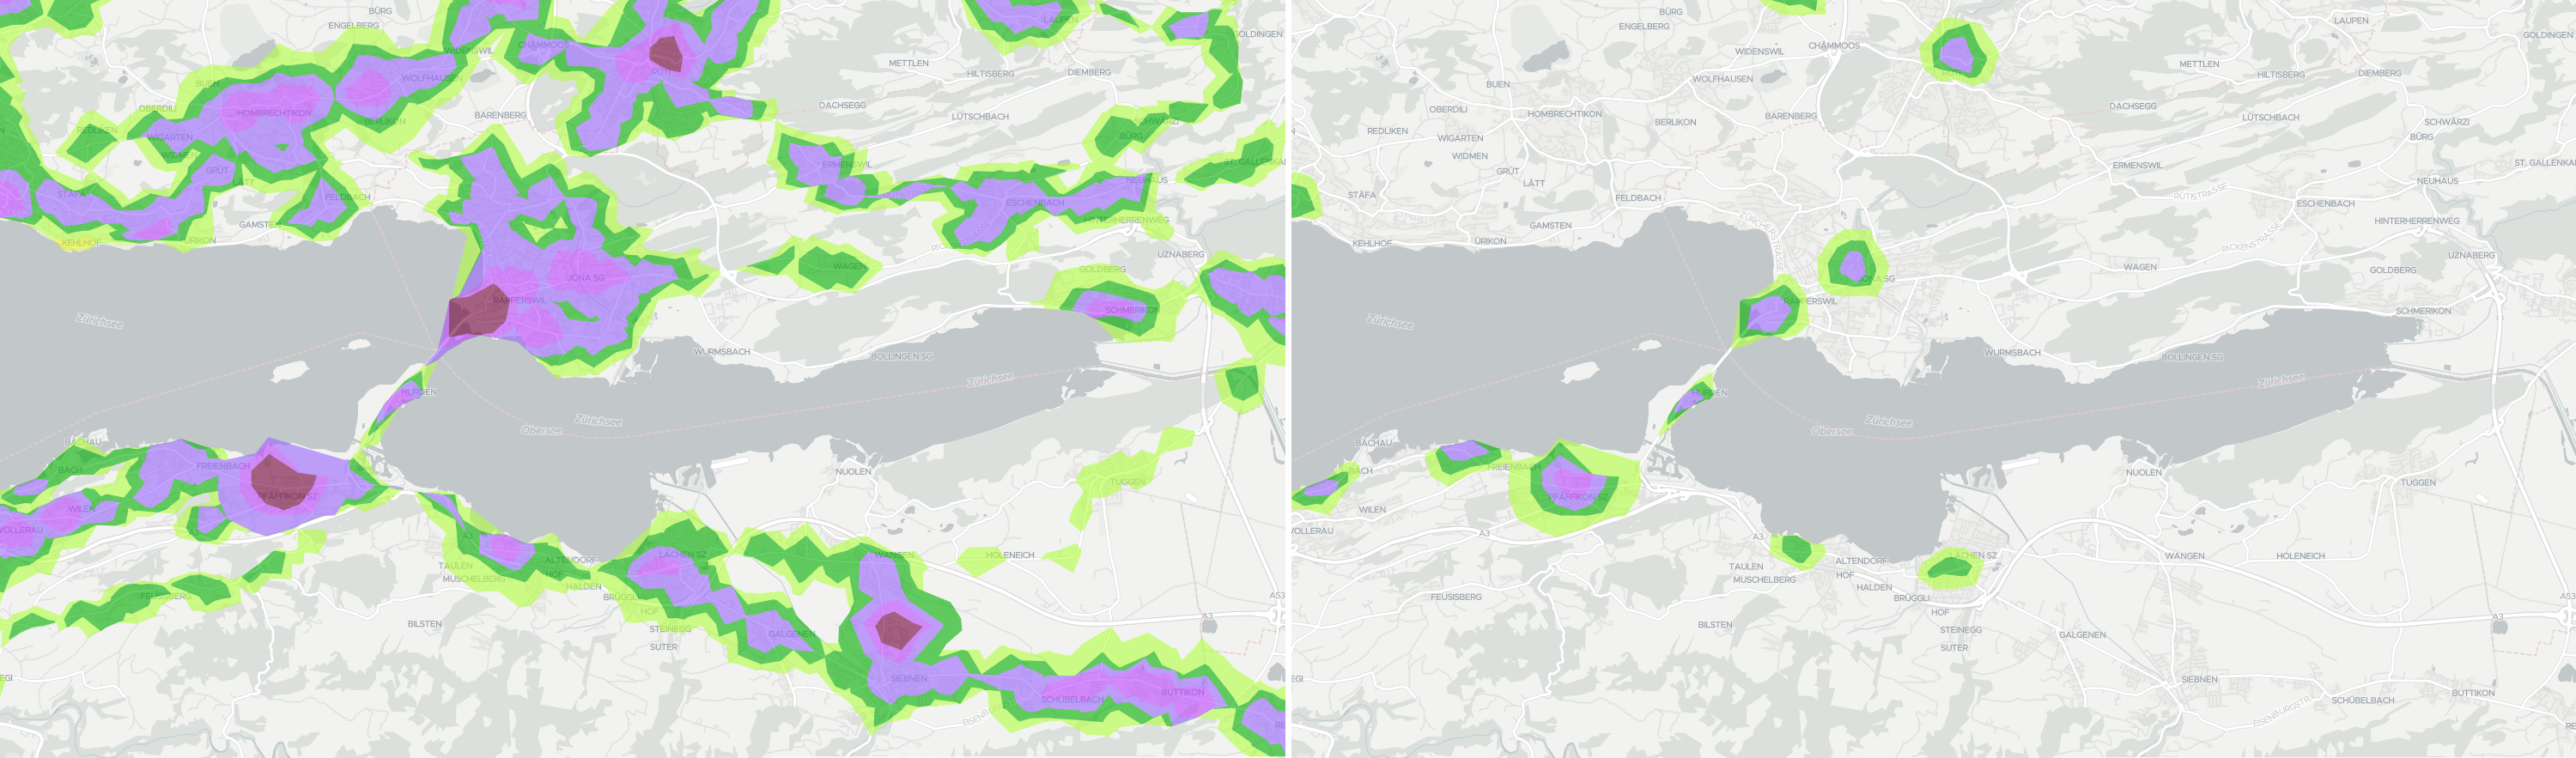
\includegraphics[width=1.0\linewidth]{technicalreport/img/due_date_comparison.png}
    \caption[Vergleich Stichtag und Zeitintervall]{Vergleich Stichtag und Zeitintervall: 10.11.2018, 06:00 - 20:00 Uhr (links) und 10.11.2018, 01:00 - 04:00 Uhr (rechts)}
    \label{fig:due_date_comparison}
\end{figure}

In Abbildung \ref{fig:due_date_comparison} sieht man den Vergleich für einen Stichtag mit unterschiedlichen Zeitintervallen, links tagsüber und rechts in der Nacht.
Anzumerken ist, dass beide mit denselben Ellen gemessen werden.
Dadurch ergeben sich in der Nacht deutlich tiefere Güteklassen als am Tag.

\subsection{Ausblick: Weiterentwicklung}
\label{Resultate:Ausblick: Weiterentwicklung}

Durch die neue Spezifikation und Web-Applikation ist die Grundlage für weitere und fortgeschrittene Auswertungen geschaffen.

Verknüpft man die neuen \gls{ÖV-Güteklassen} mit der Bevölkerungsdichte, ist es möglich, Verbesserungspotential für den \acs{ÖV} zu eruieren.
Dadurch wären Auswertungen analog zu "`95\% der wohnhaften Personen in einem bestimmten Gebiet müssen mindestens in der \gls{ÖV-Güteklassen} XYZ sein"' möglich.

Aber auch für den privaten Gebrauch ist eine Weiterentwicklung von Interesse.
So ist ein Wohnortfinder denkbar, welcher die Qualität des \acs{ÖV}-Anschlusses und anderen Faktoren (Nähe zu einer Schule oder Krankenhaus, etc.) berücksichtigt.

\paragraph{Raster-Ansatz}~\\
Für die Berechnung der Einzugsgebiete wird in dieser Arbeit der Ansatz von \glspl{Isochrone} verwendet, die entlang des Strassen- und Wegnetzes verlaufen.
Die Grundannahme dahinter ist, dass sich Fussgänger immer entlang des Wegnetzes fortbewegen.
Dabei gibt es Probleme bei offenen Fussgängerflächen, wie sie in~\cite{plaza_route} behandelt werden.
Ein anderer Ansatz basiert statt auf Routen auf einem Raster~\cite{pedestrian_accessibility_planning}. Dieser geht davon aus, dass sich Fussgänger überall fortbewegen, wo keine Hindernisse (Gebäude, Flüsse, Barrieren, etc.) sie daran hindern.
Dabei wird ein Raster über die Karte gelegt und jeder Kachel einen Kostenwert zugeordnet.
Für die Erzeugung der Einzugsgebiete werden dann vom Startpunkt aus in alle Richtungen die Kacheln eingefärbt und bei jedem Schritt die Kosten der Kachel addiert.
Dies wird so lange wiederholt, bis die gewünschten Maximalkosten erreicht werden.
In Abbildung \ref{fig:grid_based_approach} ist ein Ergebnis einer solchen Berechnung abgebildet.

\begin{figure}[ht]
    \centering
    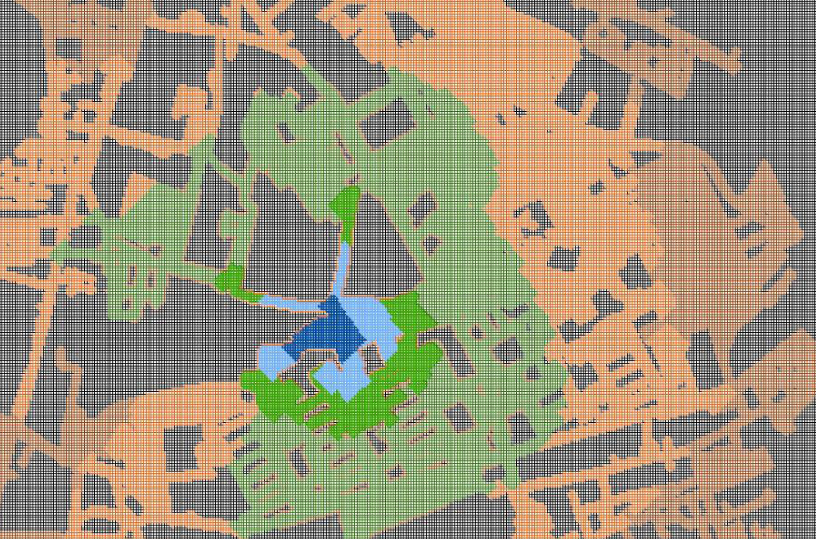
\includegraphics[width=0.6\linewidth]{start/img/grid_based_approach.png}
    \caption[Grid- beziehungsweise raster-basierter Ansatz]{Grid- beziehungsweise raster-basierter Ansatz~\cite{pedestrian_accessibility_planning}}
    \label{fig:grid_based_approach}
\end{figure}

Mit dieser Methode ist die Qualität des \glspl{Routing-Graph} und Problematiken wie bei Fussgängerflächen weniger relevant.
Für die Berechnung der \gls{ÖV-Güteklassen} ist dies ein spannender Ansatz für einen Vergleich mit der Lösung in dieser Arbeit.

\paragraph{Multimodaler Verkehr}~\\
In allen bisherigen Ansätzen zur Ermittlung von \gls{ÖV-Güteklassen} wird das Einzugsgebiet von \glspl{Haltestelle} über die Laufdistanz charakterisiert.
Dabei werden die Möglichkeiten des Individualverkehrs (wie etwa Auto, Fahrrad, etc.) nicht mit eingerechnet.
Die Maximaldistanz eines Erschliessungsgebiets liegt bei Laufdistanzen bei 15 Minuten Gehzeit.
Mit einem Fahrrad etwa wäre die Distanz deutlich grösser, die in 15 Minuten zurückgelegt werden können.
Für andere Verkehrsmittel bräuchte es daher jeweils andere Massstäbe.

Die jetzige Einschränkung auf Fussdistanzen führt auch daher, dass die \gls{ÖV-Güteklassen} nicht zu komplex werden sollen, damit eine einfache und schnelle Interpretation möglich bleibt.
Daher ist hier abzuwägen, inwiefern es sinnvoll ist, andere Arten des Individualverkehrs miteinzubeziehen.

\subsection{Dank}
\label{Resultate:Dank}

Wir möchten folgenden Personen für ihre Unterstützung und Mitwirkung bei dieser Arbeit danken:

\textbf{Prof. Stefan Keller, IFS Institut für Software,} für die Zeit, Ressourcen, Kontakte, Know-How und Unterstützung, von welcher wir jederzeit profitieren konnten.

\textbf{Prof. Claudio Büchel, IRAP Institut für Raumentwicklung}, für die initiale Idee, Know-How über Verkehrsplanung und Fachunterstützung über das gesamte Projekt.

\textbf{Mitarbeiter, IFS Institut für Software,} für den regen Know-How-Austausch und die Unterstützung bei der Produktivsetzung.


% Summary index document for ...

\chapter{SW-Projektdokumentation }
\label{SW-Projektdokumentation}


\section{Überblick}
\label{Überblick}

Der Teil \ref{Technischer Bericht} \nameref{Technischer Bericht} verfolgt das Ziel, dem Leser einen Überblick über die Problemstellung und über den Inhalt der Arbeit zu geben.
Dabei wurde dem \nameref{Stand der Technik} besondere Beachtung geschenkt und die Spezifikation "`\gls{ÖV-Güteklassen} 2018"' (Kapitel \ref{Spezifikation OeVGK18}) erstellt.
Der Teil \nameref{SW-Projektdokumentation} legt den Fokus auf deren konkreten Umsetzung.


\section{Anforderungsspezifikation}
\label{Anforderungsspezifikation}

\subsection{Use Cases}
\label{Anforderungsspezifikation:Use Cases}

Im folgenden sind die funktionalen Anforderungen an das System mit all seinen Komponenten, welche im Kapitel \ref{Architektur} aufgeführt sind, als Use Cases im Brief-Format beschrieben.
Zur Übersicht ist das Use Case Diagramm in Abbildung \ref{fig:UseCase_OeV-Gueteklassen_2018} zu betrachten.

\begin{figure}[ht]
\centering
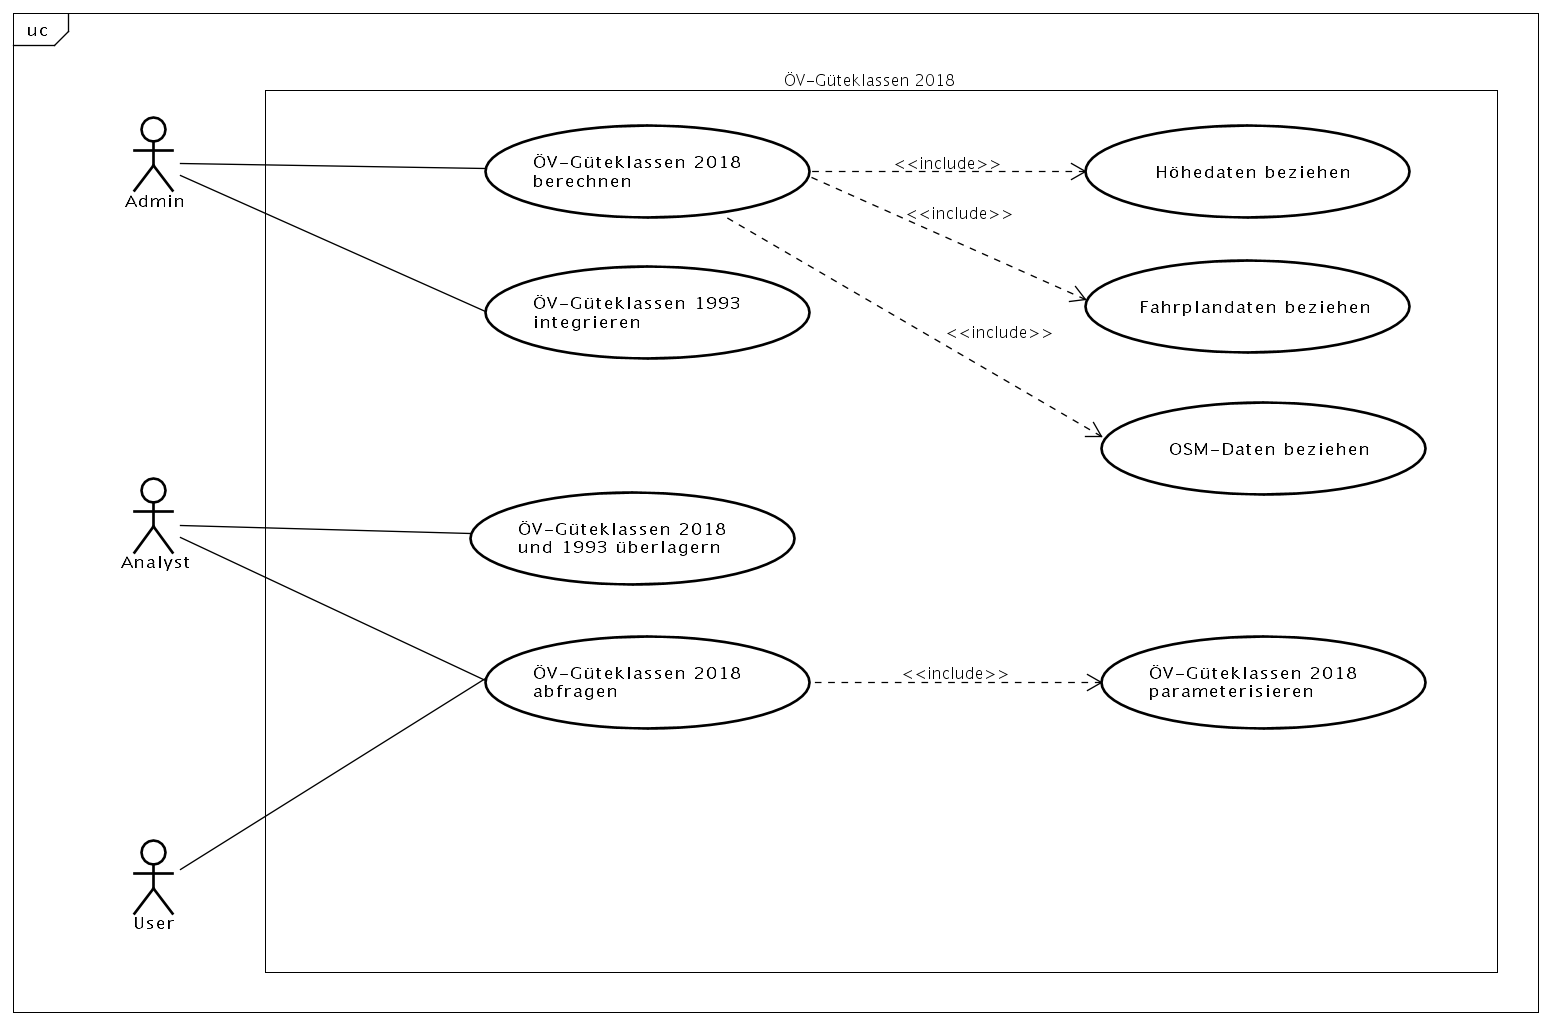
\includegraphics[width=1.0\linewidth]{projectdoc/img/UseCase_OeV-Gueteklassen_2018}
\caption[Use Case Diagramm]{Use Case Diagramm}
\label{fig:UseCase_OeV-Gueteklassen_2018}
\end{figure}

\subsubsection{Aktoren}
\label{Use Cases:Aktoren}

Um die Anforderungen akkurat evaluieren zu können, ist es essentiell, die Aktoren des Systems zu identifizieren.
In der Tabelle \ref{table:Aktoren} sind die Aktoren mit ihren Interessen aufgelistet.

\begin{longtable}{l p{14cm}}
        \toprule
        \textbf{Aktor}
                                & \textbf{Beschreibung und Interesse} \\
        \midrule
        \textbf{Admin}
                                & Ein \emph{Admin} ist für die Bereitstellung von akkuraten \acs{ÖV}-Güteklassen-Daten verantwortlich, welche er den Aktoren \emph{Analyst} und \emph{User} für die weitere Auswertung zur Verfügung stellt.
                                So möchte er die erforderlichen Daten sammeln und verarbeiten. \\
        \textbf{Analyst}
                                & Unter dem Aktor \emph{Analyst} sind Raum-/Verkehrsplaner, Transportgesellschaften und weitere Personen zusammengefasst, welche die \acs{ÖV}-Güteklassen-Daten für analytische Zwecke und als Planungsinstrument verwenden möchten. \\
        \textbf{User}
                                & Ein \emph{User} ist grundsätzlich am aktuellen Stand der \acs{ÖV}-Güteklassen in einer bestimmten Region interessiert, welche er als Basis für weitere Entscheidungen bezieht. \\
        \bottomrule
    \caption{Aktoren}
    \label{table:Aktoren}
\end{longtable}

\subsubsection{UC01: ÖV-Güteklassen 2018 berechnen}
\label{Use Cases:UC01}

Aktoren: \emph{Admin}

Include: \nameref{Use Cases:UC02}, \nameref{Use Cases:UC03}, \nameref{Use Cases:UC04}

Der \emph{Admin} startet die Berechnung der \acs{ÖV}-Güteklassen 2018 basierend auf einer Konfiguration (Stichtage und Zeitspannen) periodisch.


\subsubsection{UC02: Höhendaten vorverarbeiten}
\label{Use Cases:UC02}

Aktoren: \emph{Admin}

Der \emph{Admin} füḧrt das manuelle Beziehen der Höhendaten durch und übergibt diese dem System ''\acs{ÖV}-Güteklassen 2018''.
Das System bereit die Daten so vor, dass sie in \nameref{Use Cases:UC01} für die ''\acs{ÖV}-Güteklassen 2018''-Berechnung einbezogen werden können
Da die diese Daten nicht einem stetigen Wandel unterstehen, steht es dem \emph{Admin} frei, diesen Schritt auszulassen und bereits im System vorhandene, verarbeitete Höhendaten zu verwenden.

\subsubsection{UC03: Fahrplandaten periodisch vorverarbeiten}
\label{Use Cases:UC03}

Aktoren: \emph{Admin}

Der \emph{Admin} nutzt das System ''\acs{ÖV}-Güteklassen 2018'' für das periodische Beziehen der Fahrplandaten über eine externe Schnittstelle.
Das System bereit die Daten so vor, dass sie in \nameref{Use Cases:UC01} für die ''\acs{ÖV}-Güteklassen 2018''-Berechnung einbezogen werden können.

\subsubsection{UC04: OSM-Daten periodisch vorverarbeiten}
\label{Use Cases:UC04}

Aktoren: \emph{Admin}

Der \emph{Admin} nutzt das System ''\acs{ÖV}-Güteklassen 2018'' für das periodische Beziehen der \acs{OSM}-Daten über eine externe Schnittstelle.
Das System bereit die Daten so vor, dass sie in \nameref{Use Cases:UC01} für die ''\acs{ÖV}-Güteklassen 2018''-Berechnung einbezogen werden können.


\subsubsection{UC05: ÖV-Güteklassen 1993 integrieren}
\label{Use Cases:UC05}

Aktoren: \emph{Admin}

Der \emph{Admin} nutzt das System ''\acs{ÖV}-Güteklassen 2018'' für die Integration der bereits berechneten ÖV-Güteklassen 1993 \cite{berechnung_are}.


\subsubsection{UC06: ÖV-Güteklassen 2018 und 1993 vergleichen}
\label{Use Cases:UC06}

Aktoren: \emph{Analyst}

Der \emph{Analyst} nutzt das System ''\acs{ÖV}-Güteklassen 2018'' für den Vergleich der \acs{ÖV}-Güteklassen 1993 und 2018.
Das System präsentiert eine grafische Überlagerung der beiden \acs{ÖV}-Güteklassen.

\subsubsection{UC07: ÖV-Güteklassen 2018 abfragen}
\label{Use Cases:UC07}

Aktoren: \emph{Analyst, User}

Include: \nameref{Use Cases:UC08}

Die Aktoren \emph{Analyst} und \emph{User} nutzt das System ''\acs{ÖV}-Güteklassen 2018'', um die berechneten \acs{ÖV}-Güteklassen 2018 anzuzeigen.


\subsubsection{UC08: ÖV-Güteklassen 2018 parametrisieren}
\label{Use Cases:UC08}

Aktoren: \emph{Analyst, User}

Die Aktoren \emph{Analyst} und \emph{User} übergibt dem System ''\acs{ÖV}-Güteklassen 2018'' eine Konfiguration der anzuzeigenden \acs{ÖV}-Güteklassen 2018.
Das System ''\acs{ÖV}-Güteklassen 2018'' liefert auf Basis dieser die zugehörigen, vorgerechneten Daten.

\subsection{Nicht-funktionale Anforderungen}
\label{Anforderungsspezifikation:Nicht-funktionale Anforderungen}

Im folgenden sind die nicht-funktionale Anforderungen an das System ''\acs{ÖV}-Güteklassen 2018'' aufgelistet.
Bei der Erarbeitung wird darauf geachtet, dass die Kriterien \emph{Specific} und \emph{Measurable} aus den \emph{SMART}-Kriterien\cite{SMART} eingehalten werden.
Als Spezifikation-Template wird das bewährte Quality Attribute Scenario (QAS) des Software Engineering Institute (SEI)\cite{BassSoftwareArchitecture2012} eingesetzt.

In der Kategorie \emph{Stimulus Source} werden die Aktoren aus der Tabelle \ref{table:Aktoren} wiederverwendet.

Die erwähnten Komponenten sind im Kapitel \ref{Architektur:Component} genauer beschrieben.

\subsubsection{NFA01: Auslieferung der Komponenten als Docker-Image}
\label{NFA:NFA01}

\begin{longtable}{l p{10.6cm}}
        \toprule
        \textbf{Scenario}
                                & Auslieferung der Komponenten als Docker-Image\\
        \midrule
        \textbf{Business Goals}
                                & Deployment und Portierbarkeit gewährleisten \\
        \textbf{Relevant Quality Attributes}
                                & Maintainability, Manageability, Portability, Deployability\\
        \textbf{Stimulus Source}
                                & Admin\\
        \textbf{Stimulus}
                                & Die Generierung des Docker-Image wird gestartet\\
        \textbf{Environment}
                                & Während dem Betrieb (unabhängig vom laufenden Web-App und Backend)\\
        \textbf{Artifact}
                                & Das ganze System ''ÖV-Güteklassen 2018'' mit all seinen Komponenten\\
        \textbf{Response}
                                & Die Applikation ist als Docker-Image verfügbar, welche auf Docker Hub hochgeladen werden könnte\\  
        \textbf{Response Measure}
                                & Komponenten lassen sich als Docker-Image starten\\
                                  
        \bottomrule
    \caption{QAS NFA01}
    \label{table:nfa01}
\end{longtable}

\subsubsection{NFA02: Berechnung der ÖV-Güteklassen 2018}
\label{NFA:NFA02}

\begin{longtable}{l p{10.6cm}}
        \toprule
        \textbf{Scenario}
                                & Berechnung der ÖV-Güteklassen 2018\\
        \midrule
        \textbf{Business Goals}
                                & Aktualisierte ÖV-Güteklassen 2018 für weitere Auswertung\\
        \textbf{Relevant Quality Attributes}
                                & Performance (response time), Usability, Manageability\\
        \textbf{Stimulus Source}
                                & Admin\\
        \textbf{Stimulus}
                                & Ausführung \nameref{Use Cases:UC01}\\
        \textbf{Environment}
                                & Während dem Betrieb (unabhängig vom laufenden Web-App und Backend)\\
        \textbf{Artifact}
                                & ÖV-Güteklassen 2018 Processor und seine abhängige Fremdsysteme\\
        \textbf{Response}
                                & Berechnete ÖV-Güteklassen 2018 als GeoJSON\\  
        \textbf{Response Measure}
                                & Die ÖV-Güteklassen 2018 lassen sich innerhalb von 2 Stunden nach Absetzen des Befehls über ein CLI berechnen\\                                
        \bottomrule
    \caption{QAS NFA02}
    \label{table:nfa02}
\end{longtable}

\subsubsection{NFA03: Periodische Aktualisierung der ÖV-Güteklassen 2018}
\label{NFA:NFA03}

\begin{longtable}{l p{10.6cm}}
        \toprule
        \textbf{Scenario}
                                & Periodische Aktualisierung der ÖV-Güteklassen 2018\\
        \midrule
        \textbf{Business Goals}
                                & Automatisch aktualisierte ÖV-Güteklassen 2018 für weitere Auswertung\\
        \textbf{Relevant Quality Attributes}
                                & Administrability\\
        \textbf{Stimulus Source}
                                & Cron-Job\\
        \textbf{Stimulus}
                                & Periodische Ausführung \nameref{Use Cases:UC01} \\
        \textbf{Environment}
                                & Während dem Betrieb (unabhängig vom laufenden Web-App und Backend)\\
        \textbf{Artifact}
                                & ÖV-Güteklassen 2018 Processor und seine abhängige Fremdsysteme\\
        \textbf{Response}
                                & Berechnete ÖV-Güteklassen 2018 als GeoJSON\\  
        \textbf{Response Measure}
                                & Alle zwei Wochen liegt eine aktualisiertes GeoJSON bereit, welches von anderen Komponenten verwendet werden kann\\                                
        \bottomrule
    \caption{QAS NFA03}
    \label{table:nfa03}
\end{longtable}

\subsubsection{NFA04: Dauer des Unterbruchs bei Integration aktualisierter Daten}
\label{NFA:NFA04}

\begin{longtable}{l p{10.6cm}}
        \toprule
        \textbf{Scenario}
                                & Dauer des Unterbruchs bei Integration aktualisierter Daten\\
        \midrule
        \textbf{Business Goals}
                                & Kurzer Unterbruch während des Einspielens aktualisierter Daten\\
        \textbf{Relevant Quality Attributes}
                                & Availability \\
        \textbf{Stimulus Source}
                                & Admin\\
        \textbf{Stimulus}
                                & Nach Ausführung von \nameref{Use Cases:UC01} und \nameref{Use Cases:UC05} durch manuelle Interaktion des Admin\\
        \textbf{Environment}
                                & Web-App und Backend ist heruntergefahren\\
        \textbf{Artifact}
                                & Web-App und Backend\\
        \textbf{Response}
                                & Web-App ist nicht verfügbar und Backend wird mit aktualisierten ''ÖV-Güteklassen 2018''-Daten gestartet\\  
        \textbf{Response Measure}
                                & Web-App ist nicht länger als eine Stunde vom Zeitpunkt des Herunterfahrens nicht verfügbar\\                                
        \bottomrule
    \caption{QAS NFA04}
    \label{table:nfa04}
\end{longtable}

\subsubsection{NFA05: Antwortzeit ÖV-Güteklassen 2018 anzeigen}
\label{NFA:NFA05}

\begin{longtable}{l p{10.6cm}}
        \toprule
        \textbf{Scenario}
                                & Antwortzeit ÖV-Güteklassen 2018 anzeigen\\
        \midrule
        \textbf{Business Goals}
                                & \\
        \textbf{Relevant Quality Attributes}
                                & Performance (response time), Scalability\\
        \textbf{Stimulus Source}
                                & User, Analyst\\
        \textbf{Stimulus}
                                & Ausführung \nameref{Use Cases:UC06} oder \nameref{Use Cases:UC07}\\
        \textbf{Environment}
                                & Normaler Betrieb\\
        \textbf{Artifact}
                                & Web-App und Backend\\
        \textbf{Response}
                                & ÖV-Güteklassen 2018 werden für den gewünschten Bereich angezeigt\\  
        \textbf{Response Measure}
                                & ÖV-Güteklassen 2018 werden nach Verändern des Zooms innerhalb von 5 Sekunden angezeigt\\                                
        \bottomrule
    \caption{QAS NFA05}
    \label{table:nfa05}
\end{longtable}



\section{Analyse}
\label{Analyse}

\subsection{Routing Engine}
\label{Analyse:Routing Engine}

In den Rahmenbedingungen (Kapitel \ref{Einführung:Rahmenbedingungen, Umfeld, Definitionen, Abgrenzungen}) wurde festgehalten, für die Implementation der "`\acs{ÖV}-Güteklassen 2018"' PostGIS~\cite{postgis} und die Routing-Engine pgRouting~\cite{pgRouting} zu verwenden, soweit diese die gewünschte Funktionalität unterstützt.
Nachfolgend soll kurz aufgezeigt werden, welche alternativen Technologien in Frage kommen und ob die technische Machbarkeit mit PostGIS/pgRouting gegeben ist.

Für die Wahl einer Routing-Engine gibt es drei grosse Open-Source Lösungen, die sich bewährt haben: OSRM~\cite{osrm}, GraphHopper~\cite{graphhopper} und pgRouting.
Für unsere Zwecke sind folgende Kriterien massgebend:

\begin{enumerate}
    \item Das Erstellen von Isochronen
    \item Die Integration von Höhendaten
\end{enumerate}

Für das Kriterium 1 bringen GraphHopper und pgRouting bereits eingebaute Funktionen mit, für OSRM gibt es ein experimentelles Tool von Mapbox~\cite{mapbox_osrm_isochrone}.

Für das zweite Kriterium, die Integration von Höhendaten, gibt es bei GraphHopper und OSRM eingeschränkte Möglichkeiten. GraphHopper bietet zwar an, das weltweit abdeckende Modell von \ac{SRTM} direkt einzubinden, dessen Genauigkeit ist mit 90 Metern aber deutlich tiefer als bei unserem swissALTI$^{3D}$-Modell mit 2--10 Metern~\cite{swissalti3d_swisstopo}. Die Integration eines eigenen Modells würde bei beiden Routing-Engines eine Anpassung der Implementation benötigen.

Bei pgRouting bringt die Implementation selbst keine direkte Unterstützung von Höhendaten mit.
Im Unterschied zu den anderen Varianten kann die Kosten-Funktion zur Berechnung von Wegzeiten aber einfach selbst angepasst werden.
Durch die Benutzung von PostgreSQL mit PostGIS bietet dieser Ansatz deutlich mehr Flexibilität.
Das Terrainmodell kann in einer separaten Datenbank effizient als Raster persistiert und für die Kostenberechnung der einzelnen Kanten abgerufen werden.

Da die Fahrplandaten ebenfalls in relationaler Form in einer PostgreSQL-Datenbank gehalten werden, wird auch die Integration dieser Daten mit dem Routing-Graphen erleichtert.

Abschliessend kann man sagen, dass die Kriterien mit pgRouting erfüllt werden und sich von den drei evaluierten Routing-Engines am besten für die Integration mit den restlichen Daten (Fahrplan- und Höhendaten) eignet.

\subsection{Evaluation Frontend-Framework}
\label{Analyse:Evaluation Frontend-Framework}

Wie in den Rahmenbedingungen (Kap. \ref{Einführung:Rahmenbedingungen, Umfeld, Definitionen, Abgrenzungen}) vorausgesetzt, stehen für die Technologie der Web-Applikation (Frontend) die Optionen React~\cite{react} oder Vue.js~\cite{vuejs} zur Auswahl.
Die Wahl viel auf diese zwei Frameworks, da sich beide momentan schnell verbreiten und zum Design von \ac{SPA} ausgelegt sind, was für unsere Zwecke zum Darstellen einer Karte gut geeignet ist.
Ein grösseres Framework wie Angular ist für unsere Anforderungen zu mächtig, weshalb die Evaluation auf diese zwei leichtgewichtigeren Varianten eingeschränkt wird.

Vue.js und React werden im Folgenden anhand mehrerer Kriterien verglichen.
Als Demonstration wird mit beiden Varianten eine identische kleine Web-Applikation entwickelt.
Diese besteht aus einer Web-Karte und einem kleinen Kontrollelement, um einen zusätzlichen Layer einzublenden.
Der Code ist auf Github~\cite{github:playground} zu finden.

Zum Schluss wird ein Fazit gezogen und entschieden, welches Framework für das Frontend eingesetzt wird.

\subsubsection{Funktionsumfang}
\label{Analyse Framework:Funktionsumfang}

Sowohl React als auch Vue.js bauen auf sehr ähnlichen Prinzipien auf.
Applikationen werden in einzelne Komponenten zerteilt und aufeinander aufgebaut.
In einer Komponente ist jeweils die Darstellung (Template) und die UI-Logik miteinander gekoppelt.
Komponenten halten intern Daten, die von einer anderen Komponente bedingt verändert werden können.

Ein Unterschied liegt in der Defintion von HTML-Templates.
Vue.js verwendet reines HTML mit einer erweiterten Template-Syntax, ähnlich wie bei herkömmlichen Template-Engines.
React dagegen benutzt JSX~\cite{jsx}, eine spezielle Syntax, bei der JavaScript und HTML gemischt werden können.
In einem Zwischenschritt wird dies zu JavaScript kompiliert, das schlussendlich HTML-Elemente erstellt.
Dies macht React etwas angenehmer, da in den Templates direkt beliebiges JavaScript eingebunden werden kann.
Bei Vue.js sind nur einzelne Expressions nötig, und der Rest der Syntax muss HTML-kompatibel sein.
So werden z.B. JavaScript-Variablen wie \code{myVar} in die HTML-kompatible Form \code{my-var} umgewandelt, was bei der Benutzung verwirrend sein kann.

React wird von Facebook entwickelt und ist etwas älter (2013) als Vue.js (2014), das unabhängig unterhalten wird.
Dadurch gibt es beim Paket-Repository von NPM mehr vorgefertigte Komponenten für React (ca. 50'000 verglichen mit ca. 10'500 für Vue.js).
Die Unterstützung und Wartung von Facebook spricht dafür, dass React auch in den nächsten Jahren stets weiter entwickelt wird.

Beide Frameworks sind aber schlank gehalten und bieten nur die Kernfunktionalitäten.
Erweiterte Komponenten wie Routing oder State-Management sind in andere Frameworks ausgelagert, welche jeweils eingebunden werden können.

Insgesamt haben React und Vue.js einen sehr ähnlichen Funktionsumfang und verwenden fast identische Prinzipien.

\subsubsection{Integration Leaflet}
\label{Analyse Framework:Integration Leaflet}

Für das Einfügen einer Web-Karte mit Raster-Kacheln in eine Web-Applikation hat sich die Library \emph{Leaflet}~\cite{leaflet} bewährt.
Es wird analysiert, wie fortgeschritten die Leaflet-Unterstützung in den jeweiligen Frameworks ist.

Für React bietet \emph{react-leaflet}~\cite{react-leaflet} die Funktionalität von Leaflet an, das Equivalent für Vue.js bildet \emph{Vue2Leaflet}~\cite{vue2leaflet}.

Beide Komponenten bieten eine rudimentäre Dokumentation an, die Bedienung wird aber erst mit den zahlreichen Beispielen klar.
Bezüglich der Funktionalität ist kein grosser Unterschied festzustellen.
\emph{Vue2Leaflet} bildet zwar nicht die komplette Leaflet-Library ab, die für diese Arbeit benötigten Funktionen sind aber alle vorhanden.


\subsubsection{Integration Vector Tiles}
\label{Analyse Framework:Integration Vector Tiles}

Vector Tiles sind Kacheln, die Ausschnitte aus Karten als Vektoren darstellen, anstatt wie bei Raster-Kacheln mit simplen Bildern~\cite{geometalab_vectortiles}.
Dies hat unter anderem den Vorteil, dass nicht bei jeder Zoomstufe ein neues Bild geladen werden muss, sondern die Vektoren beliebig vergrössert werden können.

Für die Integration solcher Vector Tiles in Webkarten hat die Firma Mapbox ein Format spezifiziert und mit \emph{Mapbox GL JS}~\cite{mapbox_gl_js} eine JavaScript-Library veröffentlicht, um diese einzubinden.
Diese Library bietet deutlich mehr Möglichkeiten als Leaflet, um die Darstellung von Kacheln individuell anzupassen.
Die Vektor-Daten selbst sind bei Mapbox bis zu einem gewissen Abrufvolumen kostenlos erhältlich.
Es können aber auch andere Datenquellen wie z.B. von OpenMapTiles~\cite{openmaptiles} verwendet werden.

Für die Integration mit React und Vue.js gibt es mehrere vorgefertigte Komponenten von Dritten.
Wir haben jeweils die beliebtesten (Anzahl Github-Stars) davon angeschaut.
Für React ist dies \emph{react-mapbox-gl}~\cite{react_mapbox_gl}, für Vue.js \emph{vue-mapbox-gl}~\cite{vue_mapbox_gl}.

Die React-Komponente ist gut dokumentiert und relativ einfach zu benutzen.
Die einzelnen Komponenten sind sauber in React-Komponenten abgebildet, was das Handling mit mehreren Layern angenehm macht.

Dagegen ist die Vue.js-Komponente nur ein einfacher Wrapper um die API von \emph{Mapbox GL JS}.
So kann z.B. ein zusätzlicher Layer nicht direkt im Template eingebunden werden, sondern muss über Event-Handling nach dem Laden der Karte hinzugefügt werden.
Dies macht das dynamische Hinzufügen und Entfernen von Karten-Elementen, was wir in unserer Applikation viel benötigen, sehr mühsam.

\subsubsection{Lernkurve}
\label{Analyse Framework:Lernkurve}

Die Lernkurve beschreibt under anderem, wie viel Zeit benötigt wird, sich in die neue Technologie einzuarbeiten.
Dies ist durchaus ein subjektives Kriterium und hängt von unserem bestehenden Erfahrung mit anderen Web-Frameworks ab.

Die beiden sehr ähnlichen Philosophien von React und Vue.js weichen in gewissen Punkten stark von uns vertrauten Praktiken ab, so etwa die inhärente Kopplung von Darstellung und Logik, die in anderen Modellen wie MVC (Model-View-Controller) aufgespalten wird.
Insofern benötigen beide Varianten eine gewisse Einarbeitungszeit, um sich mit diesen Konzepten vertraut zu machen.

Bei React kommt zusätzlich die neue Syntax JSX~\cite{jsx} dazu, die zwar etwas angenehmer zu lesen ist, aber in vielen kleinen Punkten von bereits Bekanntem abweicht.
So mussten z.B. HTML-Attribute wie \code{for} umbenannt werden, um nicht eine Namenskollision mit JavaScript zu verursachen.

Die Template-Syntax von Vue.js ist deutlich vertrauter, auch weil sie sehr dem Stil von anderen Template-Engines ähnelt.
Vue.js erlaubt auch einiges an "`Syntactic Sugar"' in den Templates.
So ist simples Data-Binding mit Event-Handling direkt im Template möglich, während bei React dies separat behandelt werden muss.

Aufgrund dieser Einschätzung kann man sagen, dass der Lernerfolg bei Vue.js schneller eintritt.

\subsubsection{Tooling}
\label{Analyse Framework:Tooling}

Da sowohl React wie auch Vue.js auf NodeJS aufsetzen und den Paketmanager NPM benutzen, ist das Tooling sehr ähnlich.

Um eine neue Applikation zu erstellen, bietet React das Tool \emph{create-react-app}~\cite{create_react_app} an.
Beim Ausführen kann man angeben, welche zusätzlichen Libraries (z.B. für Unit-Testing) man verwenden möchte.
Während der Entwicklung kann ausserdem ein lokaler Server gestartet werden, der jeweils automatisch das Browser-Fenster neu lädt, wenn sich der Source-Code geändert hat.

Vue.js bietet mit \emph{vue-cli}~\cite{vue_cli} ein ähnliches Tool an.
Um eine neue Applikation aufzusetzen, kann zwischen verschiedenen Templates gewählt werden, welche sich aufgrund der geplanten Grösse der Applikation unterscheiden.
Während der Entwicklung bietet \emph{vue-cli} die praktisch identischen Möglichkeiten wie das Tool für React.

Insgesamt kann zwischen den beiden Varianten in Sachen Tooling kein markanter Unterschied festgestellt werden.


\subsubsection{Auswertung}
\label{Analyse Framework:Auswertung}

Für die Bewertung wird jedem Kriterium einen Wert von 1 bis 6 zugewiesen, wobei 6 die Bestnote ist.
Jedes Kriterium wird anhand der Relevanz und Wichtigkeit in unserem Projekt gewichtet.

\begin{table}[ht]
    \centering
    \begin{tabular}{r l p{3cm} l l}
        \toprule
        \textbf{ID} &
        \textbf{Kriterium} &
        \textbf{Relatives Gewicht (0-1)} &
        \textbf{Vue.js} &
        \textbf{React} \\
        \midrule
        1     & \nameref{Analyse Framework:Funktionsumfang}           & 0.2           & 5 / 1.0   & 5 / 1.0  \\
        2     & \nameref{Analyse Framework:Integration Leaflet}       & 0.1           & 5 / 0.5   & 4 / 0.4  \\
        3     & \nameref{Analyse Framework:Integration Vector Tiles}  & 0.3           & 2 / 0.6   & 5 / 1.5  \\
        4     & \nameref{Analyse Framework:Lernkurve}                 & 0.2           & 4 / 0.8   & 3 / 0.6  \\
        5     & \nameref{Analyse Framework:Tooling}                   & 0.2           & 5 / 1.0   & 5 / 1.0  \\
        \bottomrule
        \multicolumn{3}{l}{\textbf{Total}}                                            & \textbf{21 / 3.9}
                                                                                                & \textbf{22 / 4.5} \\
    \end{tabular}
    \caption{Resultat der Frontend-Framework-Evaluation}
    \label{table:Resultat der Frontend-Framework-Evaluation}
\end{table}

Wie in der Tabelle \ref{table:Resultat der Frontend-Framework-Evaluation} zu sehen ist, sind React und Vue.js vor der Gewichtung der Kriterien sehr ähnlich bewertet.
Das Kriterium \nameref{Analyse Framework:Integration Vector Tiles} sorgt für den Ausschlag zu Gunsten von React.
Dieses Kriterium haben wir stark gewichtet, da die Web-Karte die Hauptkomponente unserer Web-Applikation bildet und mit \emph{Mapbox GL JS} deutlich mehr Flexibilität als Leaflet anbietet.
In diesem Punkt bieten die vorhandenen Komponenten für Vue.js nicht die gewünschte Qualität.

\subsection{ÖV-Güteklassen 2018 Generator}
\label{Analyse:ÖV-Güteklassen 2018 Generator}

Der Container \nameref{container:generator} (siehe Kapitel \ref{Architektur}) ist für die Berechnung der "`ÖV-Güẗeklassen 2018"' verantwortlich.
Umgesetzt wird diese Komponente als Python-Applikation.
Für die Kommunikation und Integration mit den Umsystemen sind einige Libraries nötig, die im Folgenden kurz diskutiert werden.

\subsubsection{Integration mit PostgreSQL}
\label{analyse_generator:Integration mit PostgreSQL}

Für die Integration der Fahrplandaten und der Routing-Engine für die Berechnung der \glspl{Isochrone} ist eine Integration mit PostgreSQL nötig.
Die Routing-Engine läuft auf pgRouting, eine Erweiterung von PostGIS, das wiederum eine Erweiterung von PostgreSQL ist.
Insofern braucht es für beide Integrationen lediglich eine Möglichkeit, mit PostgreSQL zu kommunizieren.

Dazu bietet sich bei Python die relativ neue Library \emph{records}~\cite{records} an.

Für unsere Zwecke braucht es nur simple SQL-Abfragen, da ein Grossteil der Logik mit \glspl{Stored Procedure} auf dem SQL-Server selbst umgesetzt wird.

\subsubsection{Umgang mit Geometrien}
\label{analyse_generator: Umgang mit Geometrien}

In der Business-Logik des Generators wird viel mit Geometrien gehandhabt, die schlussendlich zu den "`ÖV-Güteklassen 2018"' verabeitet werden.
Hierzu hat sich die Python-Library \emph{Shapely}~\cite{shapely} bewährt.
Diese unterstützt die \gls{GEOS}-Funktionen, die PostGIS ebenfalls implementiert.
Dadurch können mit den Geometrien die gleichen Berechnungen wie auf der Datenbank vorgenommen werden, falls dies benötigt wird.
Dies spricht somit für eine reibungslose Integration.

Ebenfalls können Geometrien mit \emph{Shapely} direkt in \gls{GeoJSON} exportiert werden.
Dies erlaubt eine einfache Serialisierung, was wiederum eine einfache Weiterverarbeitung der Resultate ermöglicht.

\subsection{Design Frontend}
\label{analyse:Design Frontend}

Für das Frontend (Web-Applikation mit React) wird für das Design des User Interface ein Entwurf in Form von Wireframes erstellt.
Das Wireframe der Standard-Ansicht ist in Abbildung \ref{fig:wireframe_main} dargestellt.
Die restlichen Wireframes sind im Anhang \nameref{appendix:wireframes} abgebildet.

\begin{figure}[ht]
    \centering
    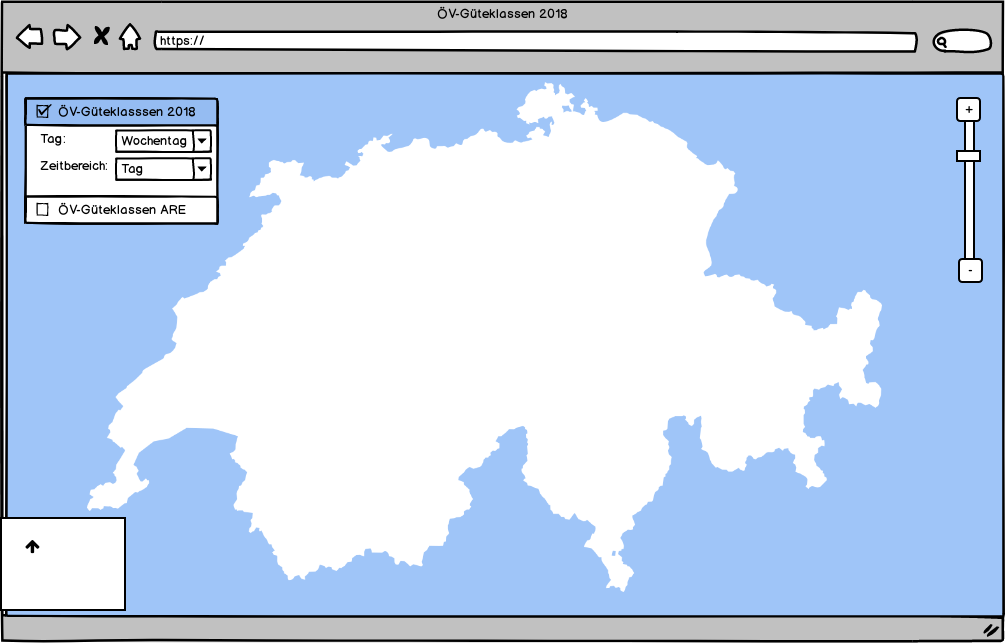
\includegraphics[width=1\linewidth]{projectdoc/img/wireframes/standardansicht.png}
    \caption[Wireframe der Standardansicht in der Web-Applikation]{Wireframe der Standardansicht in der Web-Applikation}
    \label{fig:wireframe_main}
\end{figure}

Grundsätzlich besteht das UI aus einer interaktiven Web-Karte, die sich über das gesamte Browser-Fenster erstreckt.
Darauf befindet sich ein Steuerelement, um die Anzeige der \gls{ÖV-Güteklassen} zu konfigurieren.
Die beiden Karten-Layer der Datensätze \gls{OeVGK18} und \gls{OeVGKARE} können ein- oder ausgeblendet werden.
Bei der \gls{OeVGK18} können zusätzlich Parameter wie der Tag (Wochentag oder Wochenende) sowie der Zeitbereich (Tag, Abend oder Nacht) konfiguriert werden.



\section{Architektur}
\label{Architektur}

In diesem Kapitel wird die Architektur unserer Applikation und die Schnittstellen zu den Umsystemen besprochen.
Als Anhaltspunkt wird das C4 Modell \cite{c4model} von Simon Brown verwendet.
In einem ersten Schritt wird unsere Applikation "`ÖV-Güteklassen 2018"' in den Kontext des grösseren Systems gesetzt.
Anschliessend teilen wir das System "`ÖV-Güteklassen 2018"' in einzelne Container und den zentralen Container "`ÖV-Güteklassen 2018 Generator"' in einzelne Komponenten auf.

\subsection{Systemkontext}
\label{Architektur:Systemkontext}

In Abbildung \ref{fig:system-context-diagram} ist gestrichelt eingerahmt das System "`ÖV-Güteklassen 2018"' zusammen mit den dazugehörigen Umsystemen dargestellt.
Die Pfeile bedeuten, dass ein System in Richtung der Pfeilspitze Anfragen an ein anderes System sendet.
Die Daten fliessen dementsprechend in die entgegengesetzte Richtung.

\begin{figure}[ht]
    \centering
    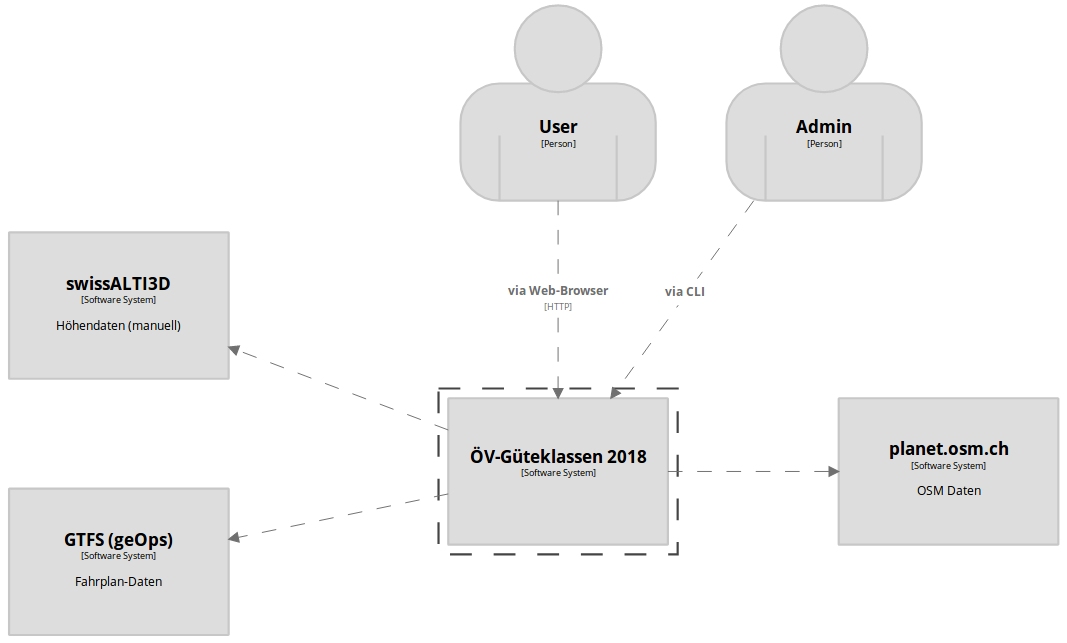
\includegraphics[width=1\linewidth]{projectdoc/img/systemcontext-diagram.png}
    \caption[Systemkontextdiagramm]{Systemkontextdiagramm ÖV-Güteklassen 2018}
    \label{fig:system-context-diagram}
\end{figure}

Im Folgenden werden die Umsysteme sowie die Beziehungen zu unserem System "`ÖV-Güteklassen 2018"' genauer beschrieben.

\subsubsection{swissALTI$^{3D}$}
\label{subsystem:swissALTI3D}

Als \gls{Terrainmodell} wird swissALTI$^{3D}$, ein Produkt von swisstopo~\cite{swissalti3d_swisstopo}, verwendet.
Dieses wird manuell vom Admin bezogen, da der Datensatz mit ca. 120GB für ein Download über das Web-\ac{API} zu gross ist und da die Daten keinem stetigem Wandel unterstellt sind.
Diese werden von swisstopo~\cite{swissalti3d_swisstopo} in einem Nachführungszyklus von 6 Jahren aktualisiert.

Das \gls{Terrainmodell} wird anschliessend in die Routing-Engine integriert, wo die Höhenunterschiede für die Kostenberechnung einer Route verwendet werden können.

\subsubsection{GTFS}
\label{subsystem:GTFS}

Die Fahrplandaten werden von der SBB regelmässig im HAFAS-Format publiziert.~\cite{sbb_hafas_spec}
Diese werden von geOps~\cite{geops_fahrplandaten} in das offene und einfacher handhabbare Format \ac{GTFS}~\cite{gtfs_spec} konvertiert und kostenfrei publiziert.~\cite{geops_fahrplandaten}
Diese können im CSV-Format für eine Speicherung in einer relationalen Datenbank bezogen werden.
Das Datenmodell ist in Abbildung \ref{fig:GTFS_data_model} ersichtlich.

\begin{figure}[ht]
    \centering
    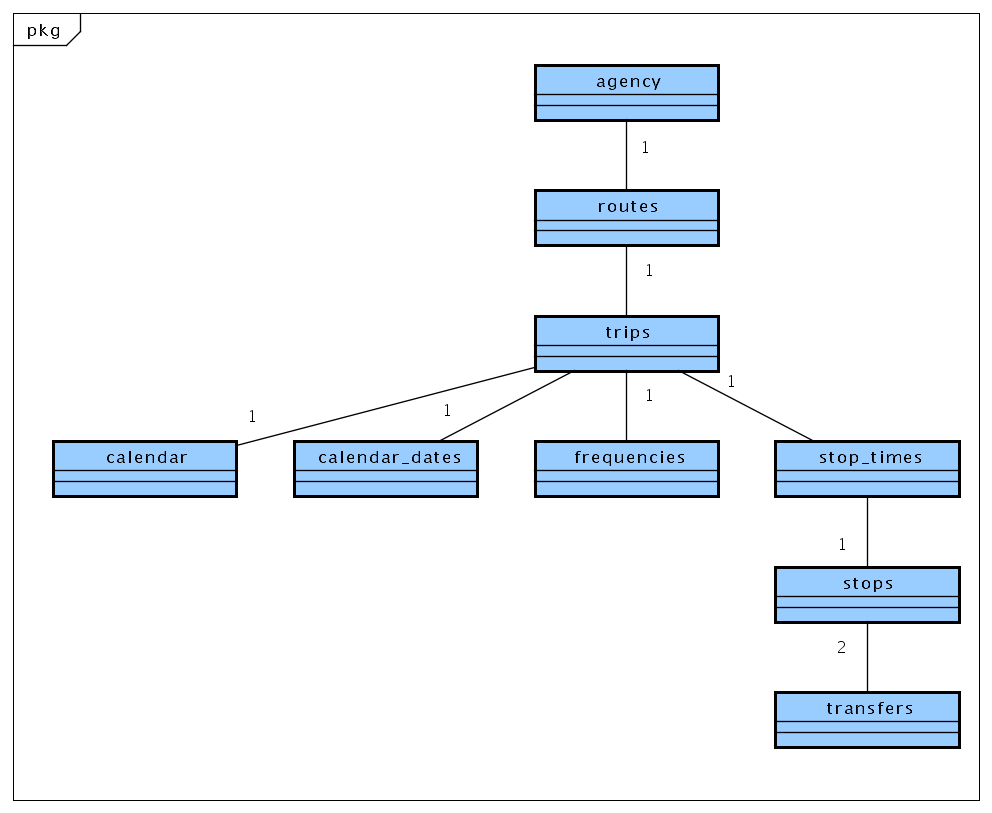
\includegraphics[width=1.0\linewidth]{projectdoc/img/GTFS_data_model}
    \caption[GTFS Datenmodell]{GTFS Datenmodell}
    \label{fig:GTFS_data_model}
\end{figure}

\subsubsection{planet.osm.ch}
\label{subsystem:planet.osm.ch}

Für die Berechnung der ÖV-Güteklassen benötigt es aktuelle Kartendaten, um die Erreichbarkeiten von Haltestellen entlang dem Strassennetz zu analysieren.
Dazu bieten sich Daten von \ac{OSM} ideal an, da sie frei verfügbar sind und kontinuierlich aktualisiert werden.

Unter planet.osm.ch~\cite{planet_osm_ch} werden täglich aktualisierte \ac{OSM}-Daten der ganzen Schweiz bereit gestellt.
Die Daten sind im \ac{PBF} und werden mit entsprechenden Tools in eine relationale Datenbank importiert, wo sie von einer Routing-Engine genutzt werden können.


\subsection{Container}
\label{Architektur:Container}

In der Abbildung \ref{fig:container-diagram} ist das System "`ÖV-Güteklassen 2018"', wie es in im \nameref{Architektur:Systemkontext} vorkam, in einzelne Container aufgespalten.
Im Folgenden werden die einzelnen Container genauer beschrieben.

\begin{figure}[ht]
    \centering
    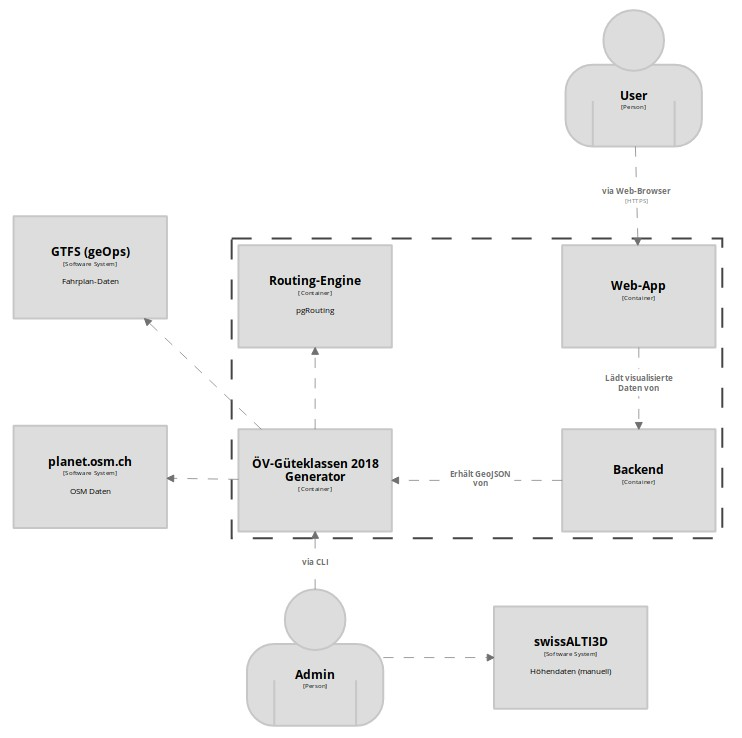
\includegraphics[width=0.8\linewidth]{projectdoc/img/container-diagram.png}
    \caption[Containerdiagramm]{Containerdiagramm ÖV-Güteklassen 2018}
    \label{fig:container-diagram}
\end{figure}
% TODO: Use Express export instead of a screenshot

\subsubsection{ÖV-Güteklassen 2018 Generator}
\label{container:generator}

Der "`\acs{ÖV}-Güteklassen 2018 Generator"' stellt das Kernstück der Berechnung der \acs{ÖV}-Güteklassen 2018 aufgrund der Spezifikation dar.
In der Abbildung \ref{fig:layer_diagram_generator} ist das Schichten-Diagramm ersichtlich.
Die Kernlogik der Berechnung befindet sich in der Schicht \nameref{layer:business}.
Der Generator agiert auf unterschiedlichen Datenquellen, so werden Fahrplandaten (\nameref{subsystem:GTFS}), ein Routing-Graphen (\nameref{subsystem:planet.osm.ch} und \nameref{container:Routing-Engine}) und ein Terrain-Modell (\nameref{subsystem:swissALTI3D}) verarbeitet und genutzt.
Die Komponente setzt voraus, dass vor dem Starten diese Daten im System vorhanden sind.
Die Integration dieser Daten ist in der Schicht \nameref{layer:integration} angesiedelt.
Die Interaktionen mit dem User sind in der Schicht \nameref{layer:ui} und die Resultate werden in der Schicht \nameref{layer:output} aufbereitet.

\begin{figure}[ht]
    \centering
    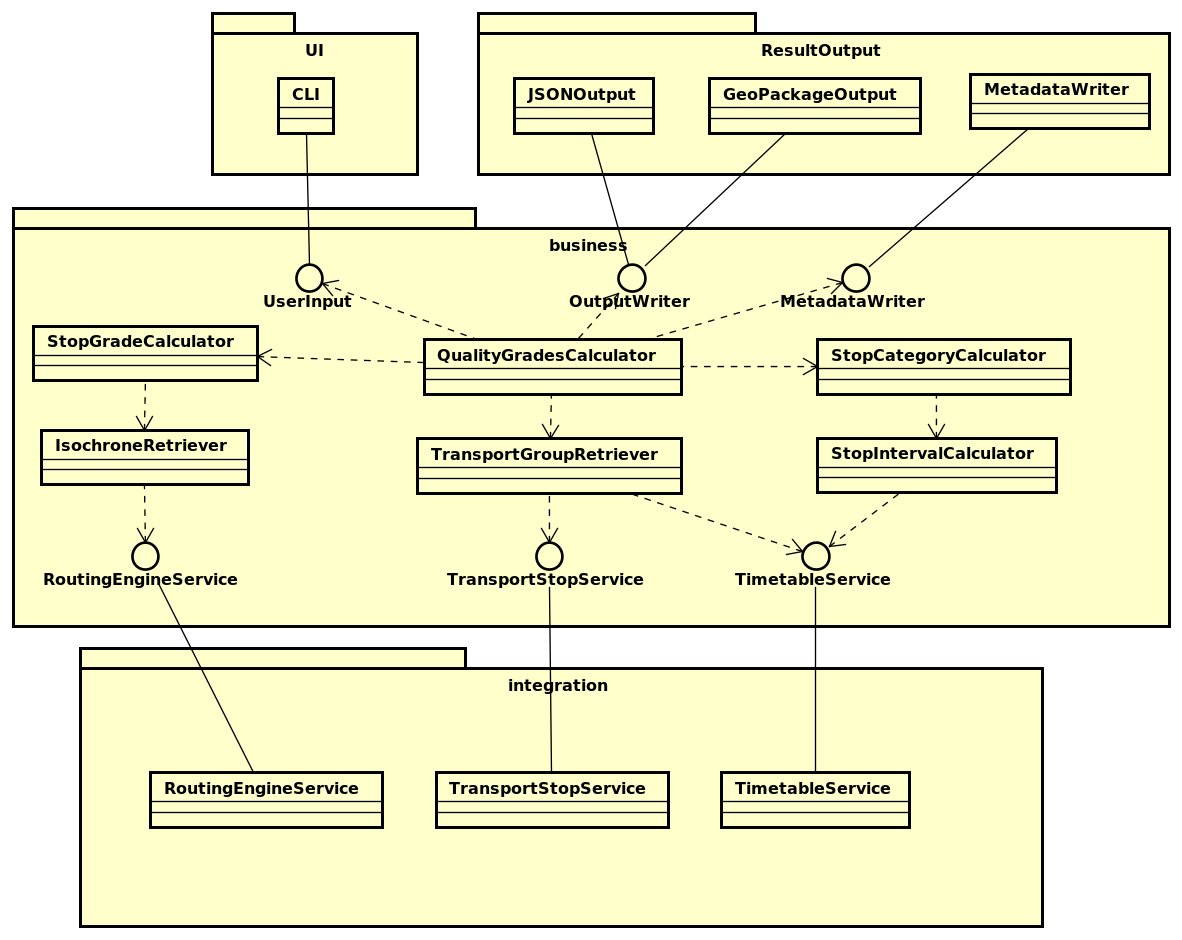
\includegraphics[width=1.0\linewidth]{projectdoc/img/guetklassen_generator_architektur.png}
    \caption[Schichten-Diagramm ÖV-Güteklassen Generator]{Schichten-Diagramm ÖV-Güteklassen Generator}
    \label{fig:layer_diagram_generator}
\end{figure}

Die Softwarearchitektur ist an die "`Clean Architecture"'-Prinzipien von \cite{martin_clean_architecture} angelehnt.
Diese Architektur hat den Vorteil, dass die Kernlogik, die business-Schicht, keine Abhängigkeiten auf die die anderen Schichten hat.
Diese Schicht ist somit absolut unabhängig.
Durch das Exponieren von Interfaces für die Schichten darüber und darunter können diese separat mit unterschiedlichen Dynamiken entwickelt werden.
So entsteht beispielsweise der Anspruch nach einem zusätzlichen Output-Format öfters als nach einer Anpassung der Berechnung der \acs{ÖV}-Güteklassen.
Durch diese Trennung kann nun die Schicht \nameref{layer:output} um einen zusätzlichen Service ergänzt werden ohne Gefahr zu laufen, dass die Kernlogik durch die Änderung unbemerkt vom bisherigen Verhalten abweicht.
Die Kernlogik erwartet grundsätzlich nur eine Implementation, welche das bereitgestellte Interface implementiert.
Wie sie dieses Interface implementiert ist der business-Schicht prinzipiell egal.
Im Folgenden werden die einzelnen Schichten beschrieben.

\paragraph{business}~\\
\label{layer:business}
In dieser Schicht ist die Kernlogik des Generators angesiedelt.
Hier wird die Berechnung der \acs{ÖV}-Güteklassen koordiniert.
So wird die Konfiguration des Users entgegen genommen und die nötigen Vorverarbeitungen und Berechnungen angestossen.
Durch die Natur der Berechnungslogik (siehe Abbildung \ref{fig:Flow_OeVGK_Brechnung}) lässt sich die Logik analog strukturieren.
Dabei wird die Haltestellekategorie, welche sich aus der Art des Verkehrsmittel und dem Kursintervall zusammensetzt über den Service \emph{StopCategoryCalculator} berechnen.
Die \acs{ÖV}-Güteklassen lassen sich in einem weiteren Schritt mithilfe des \emph{StopGradeCalculator} berechnen.
\emph{QualityGradesCalculator} übernimmt hier die Koordination der Berechnung.

\paragraph{integration}~\\
\label{layer:integration}
Alle Datenbankzugriffe erfolgen über die Integration-Schicht.
Es ist bewusst kein \acl{ORM} angedacht.
Dies aus dem Grund da intensiv mit StoredProcedures gearbeitet wird und vorallem Berechnungen auf der Datenbank durchgeführt werden und somit die Tabellen keine Objekte repräsentieren.

\paragraph{ui}~\\
\label{layer:ui}
In der ui-Schicht sind die Interaktionen mit dem User angedacht.
So ist hier ein CLI angesiedelt, welche Konfigurationen über eine einfache Bedienung entgegen nimmt.

\paragraph{output}~\\
\label{layer:output}
Die Ergebnisse der \acs{ÖV}-Güteklassen werden über diese Schicht dem User exponiert.
Der Vorteil der oben beschriebenen "`Plugin-Architektur"' macht sich hier stark sichtbar.
Entsteht das Verlangen nach einem zusätzlichen Output der \acs{ÖV}-Güteklassen als GeoPackage kann problemlos ein Service \emph{GeoPackageWriter} erstellt werden, welche das Interface \emph{OutputWriter} implementiert und analog zum \emph{GeoJSONWriter} das Resultat als GeoPackage ausliefert.
Die Kernlogik, sprich die business-Schicht muss so nicht angepasst werden.

\subsubsection{Backend}
\label{container:Backend}

Das Backend nimmt die Ergebnisse der Berechnungen vom Container \nameref{container:generator} entgegen.
Mit diesen Daten wird eine Web-\ac{API} angeboten, die dann von der \nameref{container:Web-App} verwendet wird, um die Visualisierung auf der Web-Karte zu realisieren.
Die Daten werden der Web-App im \gls{GeoJSON}-Format ausgeliefert.

% Hat das Backend noch andere Verantwortlichkeiten?

\subsubsection{Web-App}
\label{container:Web-App}

Die Web-App dient als Frontend des Systems "`\acs{ÖV}-Güteklassen 2018"'.
Die Applikation wird als \ac{SPA} direkt an den Browser des Users ausgeliefert.
Von dort werden dann per JavaScript die Daten im \gls{GeoJSON}-Format vom \ac{API} des \nameref{container:Backend}-Containers abgerufen und visualisiert.

Dafür wird, wie in den Rahmenbedingungen (Kap. \ref{Einführung:Rahmenbedingungen, Umfeld, Definitionen, Abgrenzungen}) festgehalten, entweder \emph{Vue.js}~\cite{vuejs} oder \emph{React}~\cite{react} verwendet.
Die beiden Varianten werden im Kapitel \ref{Analyse:Evaluation Frontend-Framework} evaluiert und eine Entscheidung getroffen.

\subsubsection{Routing-Engine}
\label{container:Routing-Engine}

Die Routing-Engine ist für die Berechnung von Isolinien verantwortlich.
Dazu werden zuerst periodisch die Kartendaten von \nameref{subsystem:planet.osm.ch} eingelesen und zusammen mit dem \gls{Terrainmodell} von \nameref{subsystem:swissALTI3D}, das zuvor vom Admin manuell besorgt wurde, eine Routing-Topologie erstellt.

Sobald der Admin die Berechnung der ÖV-Güteklassen auslöst, wird die Routing-Engine vom \nameref{container:generator} nach Isolinien abgefragt, die mit Haltestellen als Startpunkt und einer gewissen Distanz (gewichtet nach Höhenunterschied) berechnet werden.
Diese Isodistanzen bilden Polygone, die anschliessend vom Generator weiter verarbeitet werden.


\subsection{Code}
\label{Architektur:Code}

%TODO vlt. auf anderes Kapitel verweisen


\section{Implementation}
\label{Implementation}

In diesem Kapitel wird die Implementation der einzelnen Container beschrieben, wie sie im Kapitel \ref{Architektur:Container} definiert wurden.

\subsection{ÖV-Güteklassen 2018 Generator}
\label{Implementation:ÖV-Güteklassen 2018 Generator}

\subsubsection{Datenaufbereitung}
\label{ÖV-Güteklassen 2018 Generator:Datenaufbereitung}

Der \acs{ÖV}-Güteklassen 2018 Generator operiert auf unterschiedlichen Daten von externen Datenquellen.
Diese Daten kommen in den verschiedensten Formaten daher und müssen für eine weitere Verarbeitung gefiltert, aufbereitet und optimiert werden.
Für eine einfache Handhabung wurde ein Docker-Setup gewählt.
Die Bedienung dieses Setups ist im Kapitel \ref{Softwaredokumentation} ausführlich beschrieben.

Grundsätzlich kann man sagen, dass zwei Docker-Container existieren, namentlich \emph{tooling} und \emph{db}.
Der Docker-Container \emph{tooling} nimmt Daten in gängigen Formaten entgegen oder bezieht diese von externen Diensten und bereitet sie so vor, dass diese vom Docker-Container \emph{db} in die Datenbank \emph{oevgk18} für eine Weitereverwendung des \acs{ÖV}-Güteklassen 2018 Generator geladen werden können.
Der Docker-Container \emph{db} sorgt ebenfalls dafür, dass beim Starten die nötigen Schemas, Stored Procedures und Indizes erstellt werden.

Im weiteren sind die Services, welche die beiden Docker-Container bereitstellen, anhand eines Datenflussdiagrams aufgeschlüsselt.
Für jeden Service im Docker-Container \emph{tooling} existiert ein Pendant im Docker-Container \emph{db}, welche die vorverarbeiteten Daten des Docker-Container \emph{tooling} entgegennimmt und in die Datenbank spielt.

\paragraph{OSM-Daten}~\\
\acs{OSM}-Daten werden von der Routing-Enginge für das Berechnen von Isolinien und für das Identifizieren von \acs{ÖV}-Haltestellen verwendet.
In Abbildung \ref{fig:dataflow-docker-setup-osm-data} ist ersichtlich, wie der Docker-Container \emph{tooling} die \acs{PBF}-Datei der Schweiz von einem externen Dienst~\cite{planet_osm_ch} bezieht und für die zwei vorhin erwähnten Zwecke verarbeitet.

\begin{figure}[ht]
    \centering
    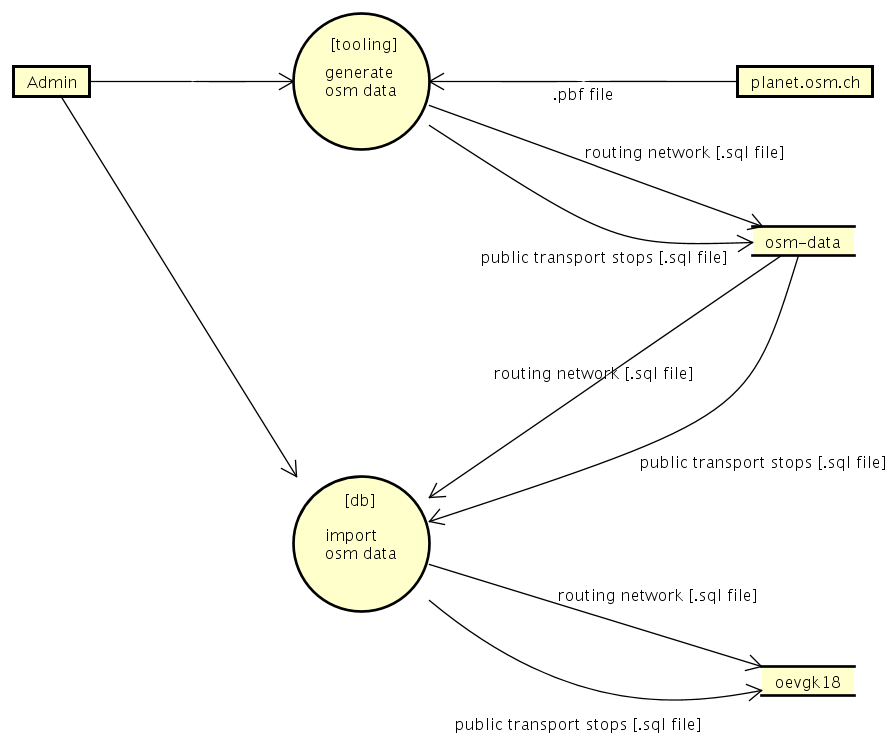
\includegraphics[width=0.8\linewidth]{projectdoc/img/dataflow-docker-setup-osm-data.png}
    \caption[Datenfluss Setup OSM-Daten]{Datenfluss Setup OSM-Daten}
    \label{fig:dataflow-docker-setup-osm-data}
\end{figure}

Das Routing-Netzwerk wird mithilfe des Tools \emph{OSM2PO}~\cite{OSM2PO} für pgrouting aufbereitet und als SQL-Datei bereitgestellt.
Die \acs{ÖV}-Haltestellen werden durch Osmosis~\cite{osmosis} gefiltert und ebenfalls in eine SQL-Datei exportiert.
Beide Tools werden durch separate Konfigurationen für unsere Zwecke konfiguriert.
So werden aus den \acs{OSM}-Daten für das Identifizieren von \acs{ÖV}-Haltestellen nur Nodes extrahiert, welche eine \emph{uic\_ref} besitzen. \ac{UIC}-Referenzen werden für die Identifizierung von \acs{ÖV}-Haltestellen verwendet.

\paragraph{GTFS-Daten}~\\
Die Fahrplandaten werden im Docker-Container \emph{tooling} von GTFS~\cite{gtfs_spec} heruntergeladen und im CSV-Format als TXT-Dateien bereitgestellt.
Diese wiederum können in einem nächsten Schritt durch den Docker-Container \emph{db} in die Datenbank gespielt werden.
Der Datenfluss ist in Abbildung \ref{fig:dataflow-docker-setup-gtfs-data} ersichtlich.

\begin{figure}[ht]
    \centering
    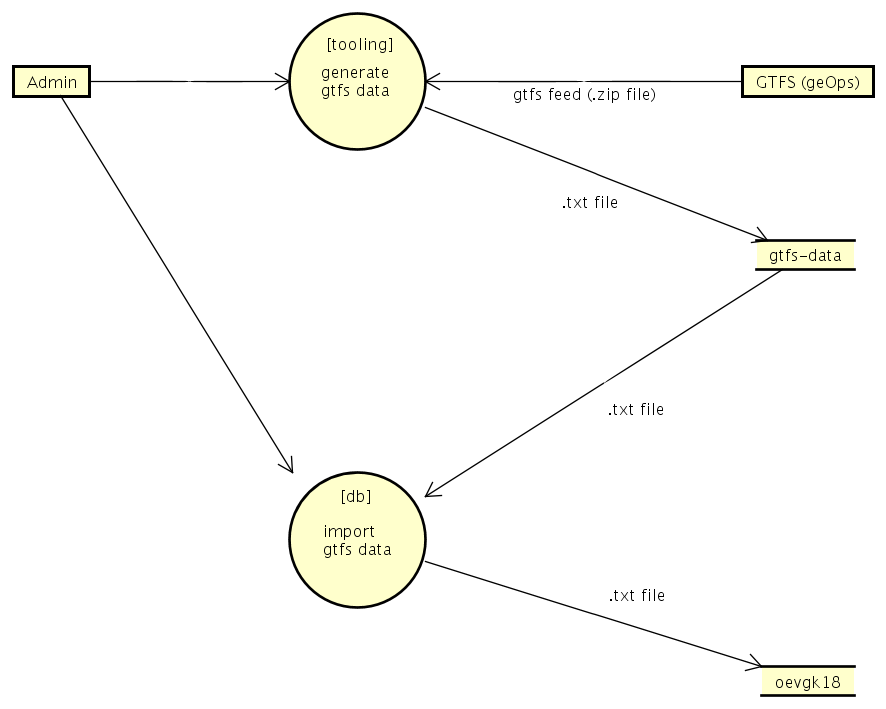
\includegraphics[width=0.8\linewidth]{projectdoc/img/dataflow-docker-setup-gtfs-data.png}
    \caption[Datenfluss Setup GTFS-Daten]{Datenfluss Setup GTFS-Daten}
    \label{fig:dataflow-docker-setup-gtfs-data}
\end{figure}

\paragraph{Terrain-Daten}~\\
Das Terrainmodell kann aufgrund der Grösse der Datei und aus lizenztechnischen Gründen nicht von einem externen Dienst bezogen und muss somit dem Service manuell als TIF-Datei bereitgestellt werden.
Diese Datei wird mit raster2pgsql~\cite{raster2pgsql}, einem Tool von PostGIS, welches Raster-Formate in ein Format konvertiert, welche in eine PostGIS-Tabelle geladen werden kann, verarbeitet.
Dieser Import wird dann vom Docker-Container \emph{db} durchgeführt.
Der Datenfluss ist in Abbildung \ref{fig:dataflow-docker-setup-terrain-data} ersichtlich.

\begin{figure}[ht]
    \centering
    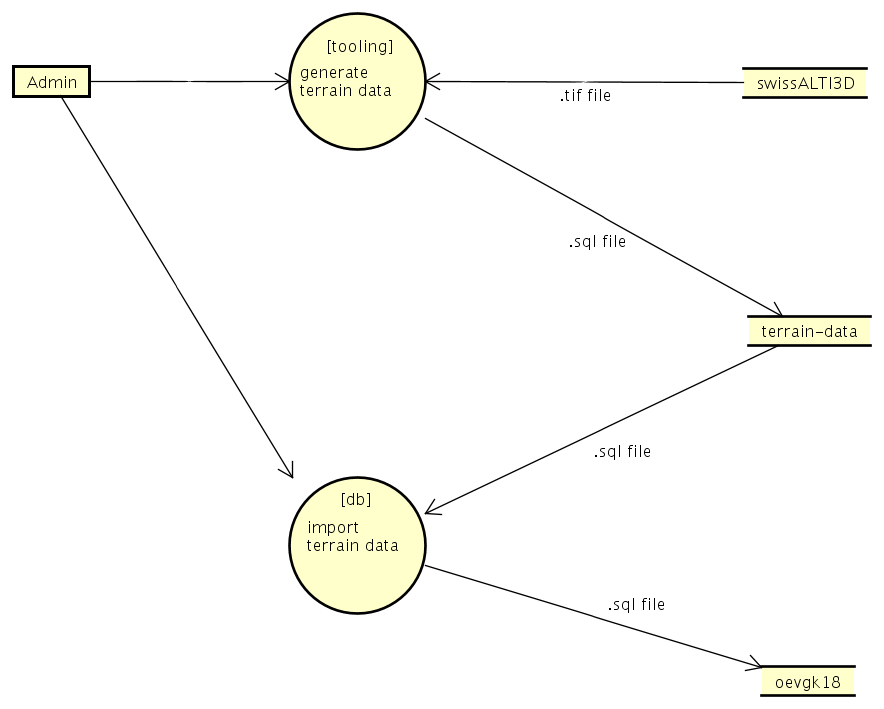
\includegraphics[width=0.8\linewidth]{projectdoc/img/dataflow-docker-setup-terrain-data.png}
    \caption[Datenfluss Setup Terrain-Daten]{Datenfluss Setup Terrain-Daten}
    \label{fig:dataflow-docker-setup-terrain-data}
\end{figure}

\subsubsection{Umsetzung Spezifikation}
\label{ÖV-Güteklassen 2018 Generator:Umsetzung Spezifikation}

\paragraph{Datenfluss}~\\
Durch die unterschiedliche Natur der Datenquellen und der Menge dieser ist es hilfreich, zu visualisieren, zu welchem Zeitpunkt, welche Daten zu welchen Zweck benötigt werden.
Wie in Abbildung \ref{fig:Flow_OeVGK_Brechnung} ersichtlich ist, werden die \acs{ÖV}-Güteklassen in fünf Schritten berechnet. 
In Abbildung \ref{fig:dataflow_OeV-Gueteklassen_2018_Generator} ist nun schematisch die Raison d’Être der Datenquellen ersichtlich.

\begin{figure}[ht]
    \centering
    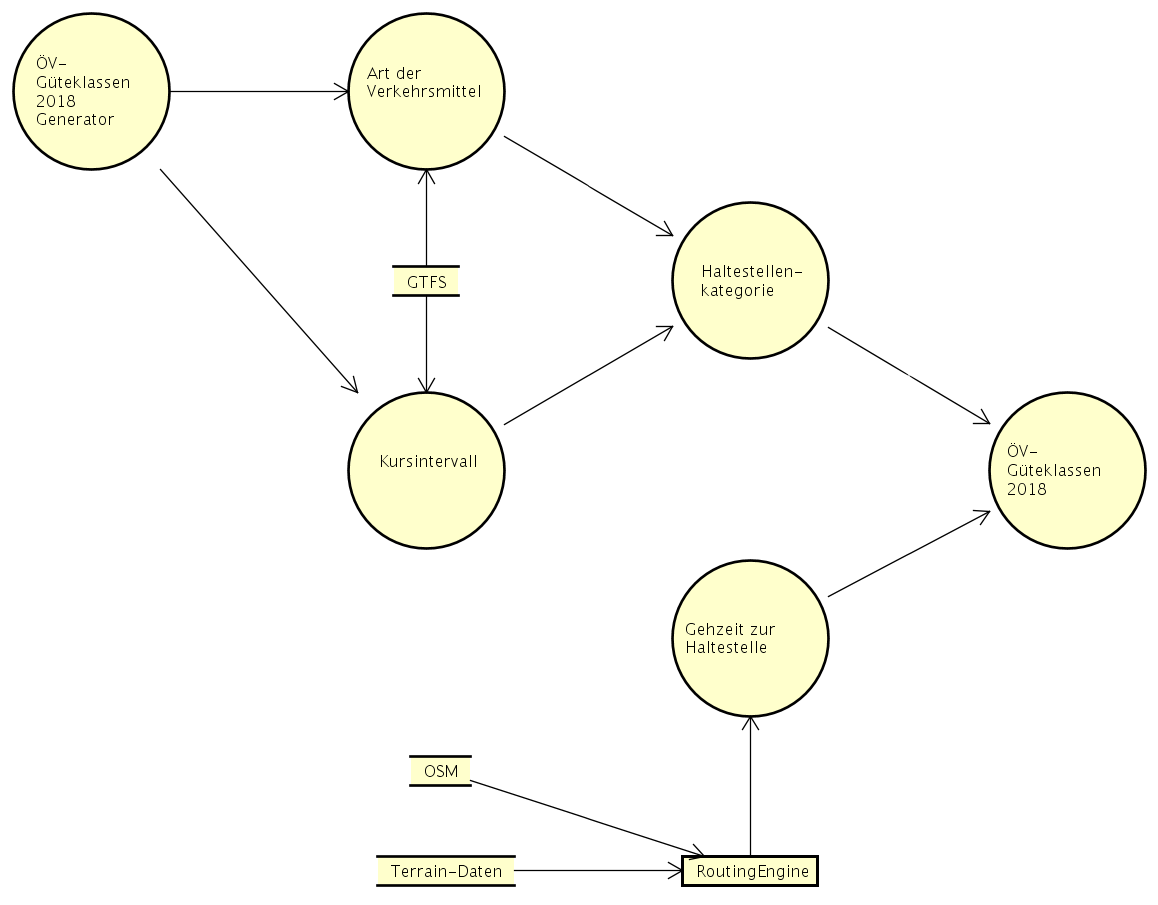
\includegraphics[width=1.0\linewidth]{projectdoc/img/dataflow_OeV-Gueteklassen_2018_Generator.png}
    \caption[Datenfluss ÖV-Güteklassen 2018 Generator]{Datenfluss ÖV-Güteklassen 2018 Generator}
    \label{fig:dataflow_OeV-Gueteklassen_2018_Generator}
\end{figure}

Die Datenquellen \emph{GTFS}, \emph{OSM} und \emph{Terrain-Daten} entsprechen an sich keinen separaten Datenquellen, sondern werden nur zum besseren Verständnis getrennt dargestellt.
Wie wir in Kapitel \ref{ÖV-Güteklassen 2018 Generator:Datenaufbereitung} gesehen haben, werden diese aufbereitet und optimiert in einer Datenbank \emph{oevgk18} gehalten.

\subsubsection{Mapping Verkehrsmittelgruppe und GTFS Route Type}
\label{ÖV-Güteklassen 2018 Generator:Mapping Verkehrsmittelgruppe und GTFS Route Type}

Die öffentlichen Verkehrsmittel werden in drei Verkehrsmittelgruppen gruppiert (siehe Kapitel \ref{Berechnungsmethodik OeVGK18:Art der Verkehrsmittel}).
Wie in Kapitel \ref{subsystem:GTFS} beschrieben, werden die Fahrplandaten im \acs{GTFS}-Format~\cite{gtfs_spec} gehalten. 
Es werden dabei 8 Verkehrsmittel-Typen definiert.
In Tabelle \ref{table:Mapping GTFS Route Type Verkehrsmittelgruppe} ist ein Mapping der definierten GTFS Route Typen und der Verkehrsmittelgruppen ersichtlich.

\begin{table}[ht]
    \centering
    \begin{tabular}[ht]{l l}
        \toprule
        \textbf{GTFS Route Type} 
                                & \textbf{Verkehrsmittelgruppe}\\
        \midrule
        0 (Tram, Streetcar, Light rail)
                                & B\\
        1 (Subway, Metro)
                                & B\\
        2 (Rail)
                                & A\\
        3 (Bus)
                                & B\\
        4 (Ferry)
                                & B\\
        5 (Cable car)
                                & (C)\\
        6 (Gondola, Suspended cable car)
                                & C\\
        7 (Funicular)
                                & C\\            
        \bottomrule
    \end{tabular}
    \caption{Mapping GTFS Route Type Verkehrsmittelgruppe}
    \label{table:Mapping GTFS Route Type Verkehrsmittelgruppe}
\end{table}


\cleardoublepage
\section{Tests}
\label{Tests}

\subsection{ÖV-Güteklassen 2018 Generator}
\label{Tests:ÖV-Güteklassen 2018 Generator}

Der Generator für die \acs{ÖV}-Güteklassen 2018 wurde in Python implementiert.
Für Unit-Tests hat sich dafür in vorhergehenden Projekten das Testing-Framework \emph{pytest}~\cite{pytest} bewährt.

Die Architektur wurde so gestaltet, dass die Business-Schicht keine direkte Abhängigkeit auf die Integrations-Schicht hat, die für die Kommunikation mit der Datenbank verantwortlich ist, und so isoliert getestet werden kann.
Die Abhängigkeiten wurden stattdessen dynamisch in einer "`Registry"', analog zu einer Dependency Injection, gehalten.
Dies erlaubte es uns, in den Unit-Tests die Module in der Integrations-Schicht durch Mocks auszutauschen.

Da einige Logik der Berechnung in Stored Procedures auf der Datenbank implementiert wurden, wäre es wünschenswert, diese ebenfalls automatisiert zu testen.
Zwar gibt es dafür Ansätze wie \emph{pgTAP}~\cite{pgTAP}, um Unit-Tests für Datenbank-Funktionen zu schreiben, bei uns war aber neben der Logik auch die Performance ein entscheidender Faktor.
Diese konnte nur manuell auf dem kompletten Datensatz der Schweiz getestet werden, denn erst dann wurde klar, welche Indizes benötigt werden und wie die Datenbank eine bestimmte Query ausführt.

Vorstellbar wären hingegen Integrations-Tests, die auf einem Test-Set die kompletten \acs{ÖV}-Güteklassen berechnen.
Die Schwierigkeit daran ist das aufwändige Setup mit Fahrplan-, Routing- und Höhendaten, die alle in einer laufenden Datenbank aufgesetzt werden müssten.
Dabei wäre es natürlich wünschenswert, das ganze Setup automatisiert in einer Continuous Integration Umgebung zu betreiben.

\subsection{Backend}
\label{Tests:Backend}

Für das Backend wurde das automatische Testing auf minimale Tests beschränkt, die prüfen, dass der Server auf API-Requests keine unerwartete Antworten liefert.
Während der Entwicklung wurde das Backend immer schlanker.
Wurden zuerst die kompletten GeoJSON-Daten für die Web-Applikation ausgeliefert, wird seit dem Wechsel zu Vector Tiles nur noch ein JSON mit Metadaten zu den Parametern eingelesen und über ein API angeboten.
Dementsprechend ist neben dem Exponieren von Metadaten keine mehr Logik vorhanden.

\subsection{Web-Applikation}
\label{tests:Web-Applikation}

\paragraph{Unit-Tests}~\\
Für das in React geschriebene Frontend wurde ursprünglich geplant, Unit-Tests mit \emph{Jest}~\cite{jest} zu schreiben.
Allerdings kam schon früh zur Entwicklung das Problem auf, dass die \emph{Mapbox GL} Komponente, die für die Basiskarte verwendet wird, nicht in einem Test geladen werden kann, weil dafür ein Browser benötigt wird.
Da die einzige Logik in der Applikation in der Verarbeitung der Metadaten vom Backend besteht, wären reine Unit-Tests aufwändig.
Sinnvoller wäre es, ein Integration-Test zusammen mit dem Backend-API zu machen.
Dies erfordert aber ein aufwändiges Setup, um dies automatisiert mit einer Continuous Integration zu verbinden.
Dieser Aufwand wäre aufgrund der Anforderungen der Web-Applikation nicht gerechtfertigt.

\paragraph{Type-Checking}~\\
Da JavaScript eine schwach typisierte Sprache ist, macht es Sinn, während der Entwicklung statisches Type-Checking zu verwenden.
So können bereits zu Beginn des Entwicklungsprozesses Fehler mit Typisierungen vermieden werden.

Dafür bietet sich die Library \emph{Flow}~\cite{flow} an, die wie React ebenfalls von Facebook entwickelt wird.
Mit dieser ist es möglich, bei allen Deklarationen die Typen anzugeben.
Kontinuierlich wird dann geprüft, dass die Typisierungen korrekt verwendet werden.



\section{Infrastruktur}
\label{Infrastruktur}

\subsection{Continuous Integration}
\label{Infrastruktur:Continuous Integration}

In unserem Projekt wird \ac{CI} einerseits für das automatische Erstellen dieser Dokumentation mit LaTeX verwendet und andererseits, um automatische Tests für die Implementation auszuführen.
Beides wird im Folgenden kurz beschrieben.

\subsubsection{Erstellen der LaTeX-Dokumentation}
\label{CI:Erstellen der LaTeX-Dokumentation}

Bei jedem Git Commit in das Repository der Dokumentation~\cite{github:thesis} wird mit Continuous Integration ein PDF erstellt.
So wird sichergestellt, dass die Dokumentation keine syntaktischen Fehler aufweist.
Das PDF wird in unser internes JIRA hochgeladen und direkt dem Task angehängt, der zum Branch gehört.

Für diese Continuous Integration haben wir uns für Travis CI ~\cite{travis-ci} entschieden, da die Integration mit Github gut funktioniert und das Produkt für Open-Source-Projekte kostenlos ist.
Allerdings bietet Travis CI keine direkte Unterstützung für eine LaTeX-Umgebung an. Die LaTeX-Pakete aus den Repositories sind ausserdem veraltet.
So muss bei jedem Build die LaTeX-Umgebung kompiliert werden, damit immer die neueste Version aller Pakete verwendet werden kann.


\subsubsection{CI für die Unit Tests}
\label{CI:CI für Backend}

Für die Continuous Integration der Web-Applikation braucht es eine Umgebung mit Node JS, um die Applikation zu kompilieren und die Tests auszuführen.
Für den \nameref{Implementation:ÖV-Güteklassen 2018 Generator} wird eine entsprechende Umgebung für Python benötigt.
Dazu bietet sich ebenfalls Travis CI~\cite{travis-ci} an.
Die entsprechenden Umgebungen sind bereits vorhanden, womit der Konfigurationsaufwand sehr klein bleibt.
Ebenfalls existiert ein Cron-Job, welcher die Builds und somit die Tests in regelmässigen Abständen ausführt.

\subsection{Deployment}
\label{Infrastruktur:Deployment}

Für das Deployment wurde eine Docker-Umgebung eingerichtet, die für die einfache Handhabung der Berechnung der \gls{ÖV-Güteklassen} 2018 dient.
Die Details dazu sind im Kapitel \ref{Implementation:ÖV-Güteklassen 2018 Generator} beschrieben.

Um die berechneten \gls{ÖV-Güteklassen} in der Web-Applikation zu visualisieren, wurde eine zusätzliche Docker-Umgebung vorbereitet.
Diese kombiniert die Web-App, Backend sowie der Tile-Server, damit man die komplette Applikation ohne zusätzliche Konfiguration lokal oder auf einem Server deployen kann.
Dies hat den Vorteil, dass das Setup, welches deployed wird, analog lokal gestartet und getestet werden kann.
Um die Services in einem gemeinsamen Endpoint zu verbinden, wird eine Nginx-Instanz als Reverse-Proxy verwendet, der die \acs{API}-Requests an die entsprechenden Endpoints weiterleitet.
Die Umgebung ist in Abbildung \ref{fig:deployment_web-app} dargestellt.

\begin{figure}[ht]
    \centering
    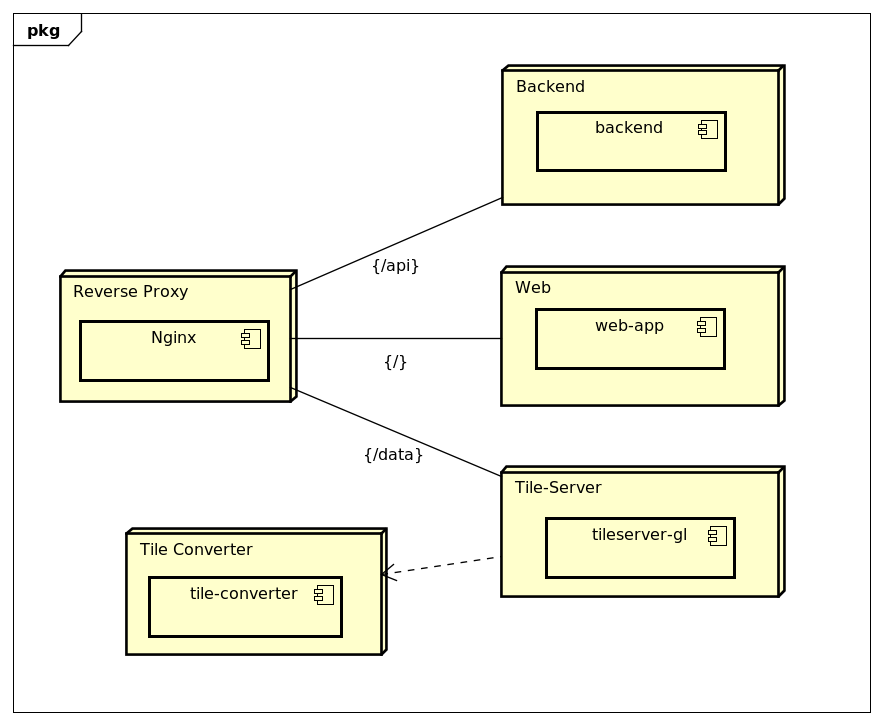
\includegraphics[width=0.8\linewidth]{projectdoc/img/deployment_web-app}
    \caption[Deployment-Diagramm der Web-Applikation]{Deployment-Diagramm der Web-Applikation mit den entsprechenden Backend-Services}
    \label{fig:deployment_web-app}
\end{figure}

Zusätzlich wurde ein Service eingerichtet, um die errechneten \gls{ÖV-Güteklassen} im \gls{GeoJSON}-Format in Map-Tiles, sprich in MBTiles (siehe Kapitel \ref{Implementation:Tile-Converter}) umzuwandeln, damit der Tile-Server damit umgehen kann.
Der Benutzer kann die \gls{GeoJSON}-Dateien in einem Ordner ablegen und die Docker-Umgebung mit Docker Compose starten.
Die Aufbereitung der Map-Tiles geschieht dann automatisch im Hintergrund.

\subsection{Version Control}
\label{Infrastruktur:Version Control}

Alle Artefakte, welche in dieser Arbeit erstellt wurden, sind öffentlich auf Github verfügbar.
Es wurde dazu eine Github Organisation mit dem Namen "`public-transport-quality-grades"'~\cite{github} erstellt.

In der Tabelle \ref{table:github_overview} sind die einzelnen Repositoriers aufgelistet und kurz der Inhalt erläutert.
Diese soll als Übersicht dienen und einen raschen Einstieg in die Version Control ermöglichen.

\begin{table}[H]
    \begin{tabular}{l p{10.6cm}}
        \toprule
        \textbf{Name}           & \textbf{Inhalt}\\
        \midrule
        thesis~\cite{github:thesis}
                                & Bachelorarbeit\\
        oevgk18-specification~\cite{github:oevgk18-specification}
                                & Aus der Bachelorarbeit extrahierte \gls{ÖV-Güteklassen} 2018 Spezifikation\\
        oevgk18-generator~\cite{github:oevgk18-generator}
                                & \gls{ÖV-Güteklassen} 2018 Generator\\
        web-app~\cite{github:web-app}
                                & Web-Applikation zur Visualisierung der \gls{ÖV-Güteklassen} 2018\\
        backend~\cite{github:backend}
                                & Backend der \gls{ÖV-Güteklassen} 2018\\
        backend-api~\cite{github:backend-api}
                                & Dokumentation des Web-\acs{API} des Backend\\
        admin~\cite{github:admin}
                                & Sitzungsprotokolle und Entscheidungen\\
        infrastructure~\cite{github:infrastructure}
                                & Interne Projekt-Infrastruktur (Jira-Setup, \dots)\\  
        playground~\cite{github:playground}
                                & Spielwiese für die Evaluation von Frameworks\\
                                
        \bottomrule
    \end{tabular}
    \caption{Github Repository Übersicht}
    \label{table:github_overview}
\end{table}

% Resultate und Ergebnisse der Arbeit. Dieser Abschnitt richtet sich an den speziell für das entsprechende Fachgebiet interessierten Ingenieur. Er soll es ihm ermöglichen, die für die Problemlösung gemachten Überlegungen zu verstehen und nachzuvollziehen.

\section{Resultate und Weiterentwicklung}
\label{Resultate und Weiterentwicklung}

%TODO

\subsection{Resultate}
\label{Resultate und Weiterentwicklung:Resultate}

\subsubsection{Laufzeit}
\label{Resultate und Weiterentwicklung:Laufzeit}

Um die Laufzeit für das Berechnen der \acs{ÖV}-Güteklassen 2018 auszuwerten, wird zuerst für die Kernoperation die theoretische Komplexität bestimmt.
Mit einer Messung wird dann die reale Laufzeit ermittelt und ausgewertet.

\paragraph{Theoretische Laufzeit}\label{Laufzeit:Theoretische Laufzeit}~\\
Für die Bestimmung der theoretischen Laufzeit wird lediglich das Berechnen der \glspl{Isochrone} betrachtet, da dies für die eigentliche Berechnung der \acs{ÖV}-Güteklassen die Kernfunktion darstellt, die am meisten Laufzeit benötigt.

Wie in \ref{ÖV-Güteklassen 2018 Generator:Umsetzung Spezifikation} beschrieben, wird für jede der $N$ Haltestellen eine oder mehrere \glspl{Isochrone} erzeugt.
Dieser Algorithmus besteht aus zwei Teilen.
Als erstes werden mit dem Dijkstra-Algorithmus~\cite{dijkstra_algorithm} alle Vertices ermittelt, die von der Haltestelle aus in einer festgelegten Zeit im Routing-Graphen erreichbar sind.
Im zweiten Schritt wird mit diesen Vertices eine Alpha Shape~\cite{alpha_shapes} erzeugt, die alle gefundenen Punkte in einem Polygon einschliesst.
Der erste Schritt muss pro Haltestelle nur ein Mal für die grösste Distanz durchgeführt werden, für die Erzeugung der \glspl{Isochrone} für kürzere Distanzen wird das Ergebnis des Dijkstra-Algorithmus gefiltert.

Der Dijkstra-Algorithmus wird in pgRouting mit der "`Boost Graph"'-Library~\cite{boost_graph} implementiert und hat eine Laufzeit von $\mathcal{O}(V \log V + E)$, wobei $E$ die Anzahl der Kanten und $V$ die Anzahl Vertices im Routing-Graphen bezeichnen.
Für eine effizientere Berechnung werden in einem vorhergehenden Schritt alle Kanten $E\prime$ ermittelt, die maximal 1300 Meter von der Haltestelle entfernt sind.
Diese Vorselektion der Kanten ist dank einem R-Tree-Index mit $\mathcal{O}(\log E)$ möglich.
Insgesamt ergibt dies eine Laufzeit von $\mathcal{O}(\log E) + \mathcal{O}(V \log V + E\prime)$.
Da die Vorselektion der Kanten $E\prime$ nur sehr klein ist ($E\prime \ll V$) und in konstanter Zeit läuft, kann dies vernachlässigt werden.

Der zweite Schritt, das Erstellen der Alpha Shape, wird nur noch mit den vorher ermittelten Punkten $V\prime$ durchgeführt.
Da dies im Vergleich zum kompletten Graphen nur sehr wenige Punkte sind ($V\prime \ll V$), ist dieser Schritt für die Laufzeit ebenfalls zu vernachlässigen.

Diese Berechnung der \glspl{Isochrone} wird für alle $N$ Haltestellen durchgeführt.
Insgesamt ergibt das folgende Laufzeit:
\[
    \mathcal{O}(N (\log E + V \log V))
\]

\begin{conditions}
    $N$   &   Anzahl Haltestellen\\
    $V$   &   Anzahl Vertices im Routing-Graph\\
    $E$   &   Anzahl Knoten im Routing-Graph\\
\end{conditions}

\paragraph{Reale Messung der Laufzeit}~\\
Um einen Richtwert für die effektive Laufzeit der Berechnung zu haben, wird auf einem Test-Computer der komplette Ablauf vom Datenimport bis zur Ausgabe der \acs{ÖV}-Güteklassen 2018 als GeoJSON durchlaufen und die Zeit gemessen.

\subparagraph{Testumgebung}
Die Messung wird auf einem Desktop-Computer mit einem Intel Xeon E3-1245 mit 3.4 GHz und 16 GB Arbeitsspeicher durchgeführt.
Als Betriebssystem wird Linux verwendet, das Terrain-Modell ist auf einer externen Festplatte im TIF-Format abgelegt.

\subparagraph{Ergebnis}

Die gemessene Laufzeiten sind in Tabelle \ref{table:Ergebnis_Laufzeitmessung} ersichtlich.
Es fällt auf, dass die Vorbereitung zur eigentlichen Berechnung die meiste Zeit beansprucht.
Dies liegt unter anderem daran, dass diese Vorbereitungsschritte externe Funktionen aufrufen, die nicht spezifisch optimiert werden können.
So braucht etwa das Berechnen der Topologie nach der Graph-Segmentierung fast zwei Stunden.
Dabei wird lediglich die eingebaute Funktion von pgRouting aufgerufen, die wohl nicht sehr effizient implementiert ist.
Als Optimierung ist vorstellbar, die Topologie direkt während der Routing-Graph-Segmentierung zu aktualisieren, was aber deutlich komplexer als die jetzige Lösung wäre.

Die eigentliche Berechnung der \acs{ÖV}-Güteklassen konnte mit Indizes auf der Datenbank und Optimierung der Algorithmen auf eine Laufzeit von rund 70 Minuten gebracht werden.
Dafür wurde während der Entwicklung kontinuierlich optimiert, in früheren Iterationen dauerte die Berechnung noch mehrere Tage.
Als Beispiel dafür sei die Optimierung zu erwähnen, den Dijkstra-Algorithmus für die Berechnung der \glspl{Isochrone} für jede Haltestelle nur ein Mal für die weiteste Distanz zu verwenden statt für jede \gls{Isochrone} einzeln.
Allein durch diese Optimierung konnte die Laufzeit zur Berechnung einer Haltestelle von ca. 450 ms auf 30 ms reduziert werden, womit die totale Laufzeit von 18 Stunden auf rund 70 Minuten gekürzt wurde.

\begin{table}[H]
    \centering
    \begin{tabular}[H]{l l}
        \toprule
        \textbf{Berechnungsschritt}
                                & \textbf{Benötigte Zeit}\\
        \midrule
        \textbf{Datenimport}
                                & \textbf{1 h 45 min} \\
        \hspace{3mm} Fahrplandaten importieren
                                & \hspace{3mm} 4 min \\
        \hspace{3mm} Routingdaten importieren
                                & \hspace{3mm} 16 min \\
        \hspace{3mm} Terrain-Modell importieren
                                & \hspace{3mm} 1 h 25 min \\
        \midrule
        \textbf{\acs{ÖV}-Güteklassen berechnen}
                                & \textbf{4 h 56 min} \\
        \hspace{3mm} Routing-Graph segmentieren
                                & \hspace{3mm} 38 min \\
        \hspace{3mm} Topologie neu berechnen
                                & \hspace{3mm} 1 h 53 min \\
        \hspace{3mm} Terrain-Daten in Routing-Graph rechnen
                                & \hspace{3mm} 1 h 13 min \\
        \hspace{3mm} \acs{ÖV}-Güteklassen für 6 Stichtage berechnen
                                & \hspace{3mm} 1 h 12 min \\
        \midrule
        \textbf{Gesamt}
                                & \textbf{6 h 41 min} \\
        \bottomrule
    \end{tabular}
    \caption{Ergebnis der Laufzeitmessung}
    \label{table:Ergebnis_Laufzeitmessung}
\end{table}


\subparagraph{Auswertung mit theoretischer Laufzeit}
Im Absatz \nameref{Laufzeit:Theoretische Laufzeit} wurde die theoretische Laufzeit zur Berechnung von \glspl{Isochrone} ermittelt.
In der Messung hat sich ergeben, dass für einen einzelnen Stichtag die Berechnung dieser \glspl{Isochrone} ca. 12 Minuten benötigt.

Mit der theoretischen Laufzeit von $\mathcal{O}(N (\log E + V \log V))$ gibt es $N = 24'318$ Haltestellen sowie $E = 7'040'965$ Kanten und $V = 6'640'003$ Vertices im Routing-Graphen.
In der Messung dauerte die Berechnung für jede der $N$ Haltestellen durchschnittlich ca. 30 ms, was einer Gesamtlaufzeit von ca. 12 Minuten entspricht.
Diese Berechnung wurde für 6 verschiedene Stichtage und Zeitintervalle durchgeführt.
Dabei ist anzumerken, dass in der Messung dieser Operation einige Variablen vernachlässigt wurden, wie etwa die Zeit für die Anfrage und Antwort des Datenbank-Servers.

\subsection{Möglichkeiten der Weiterentwicklung}
\label{Resultate und Weiterentwicklung:Möglichkeiten der Weiterentwicklung}

%TODO

% Aufwandschätzung, Zeitplan, Projektplan

\section{Projektmanagement}
\label{Projektmanagement}

\subsection{Vorgehen}
\label{Projektmanagement:Vorgehen}

Für die Bachelorarbeit wurde das agile Vorgehen SCRUM in Kombination mit Elementen von \ac{RUP} gewählt.
Gründe für diese Entscheidung sind, dass das agile Vorgehen der noch zu Beginn offenen Spezifikation der \acs{ÖV}-Güteklassen und der theoretischen Aufarbeitung entgegenkommt, welche dann iterativ finalisiert werden kann und dass der theoretische Fokus der Arbeit so besser gehandhabt und schneller reagiert werden kann.
Die wöchentlichen Besprechungen und Reviews mit dem Betreuer ist ein weiterer Grund für diese Entscheidung.
Die Kombination mit Elementen von \ac{RUP} ermöglicht es, dass Projekt in einzelne Phasen aufzuteilen, um so das Ziel und die Zeit nicht aus den Augen zu verlieren und den theoretischen Teil und die Spezifikation zu einem Abschluss bringen zu können.

\subsubsection{Entwicklung}
\label{Vorgehen:Entwicklung}

Der Source-Code der Implementation wie auch diese Arbeit wird mit Git verwaltet und ist auf Github~\cite{github} abgelegt.
Die Entwicklung und das Dokumentieren erfolgt nach dem Github-Flow.
Der Master-Branch ist auf allen Repositories während der ganzen Zeit gesperrt, so dass er nur über Pull-Requests bearbeitet werden kann.
Für jedes Arbeitspaket wird ein Branch erstellt.
Ist das Arbeitspaket implementiert, wird ein Pull-Request erstellt und dem anderen Projekt-Mitglied zum Review übergeben.
Wird der Pull-Request akzeptiert, wird der Feature-Branch in den Master gemerged.
Dieses Vorgehen hat den Vorteil, dass alle Änderungen, welche in den Master gelangen, ein Review durchlaufen müssen und so die Qualität hochgehalten werden kann.


\subsection{Zeitplanung}
\label{Projektmanagement:Zeitplanung}

Die Arbeitspakte und Zeit wird mithilfe von Jira verwaltet.
Für alle Tätigkeiten werden Arbeitspakete im Backlog erfasst, priorisiert und geschätzt.
Die Schätzung der Arbeitspakete erfolgte mit Story Points.
Die Arbeitszeitverbuchung wurde auf Arbeitspaket-Stufe mit Stunden gemacht.

\subsubsection{Phasen / Iterationen und Meilensteine}
\label{Zeitplanung:Phasen / Iterationen und Meilensteine}

Die Bachelorarbeit wird in die \ac{RUP}-Phasen (Inception, Elaboration, Construction, Transition) aufgeteilt.
Dabei wird jedoch eine von der gängigen Norm abweichende Aufteilung gewählt.
Durch den theoretischen Fokus der Arbeit und der zu erarbeitenden Spezifikation wird der Elaboration das grösste Zeitbudget zugeordnet.
Dies ist auch der Grund, warum mit einwöchigen Sprints gearbeitet wird.
In den letzten zwei Wochen des Projekts wird der Aufwand pro Sprint verdoppelt (40h pro Person), da in dieser Zeit Vollzeit am Projekt gearbeitet werden kann.
Die in Tabelle \ref{table:Phasen / Iterationen und Meilensteine} definierten Meilensteine werden in Jira als Epics definiert und die Arbeitspakete diesen zugewiesen.
Dies aus dem einfachen Grund, da Jira das Konzept Milestones nicht einfach unterstützt.

\begin{landscape}
\begin{longtable}{l p{6.5cm} p{6.5cm} p{6.5cm}}
        \toprule
        \textbf{Sprint}
                                & \textbf{Sprint 1}
                                & \textbf{Sprint 2}
                                & \textbf{Sprint 3} \\

        \midrule
        \textbf{Phase}
                                & Inception
                                & Elaboration
                                & Elaboration \\

        \textbf{Milestones}
                                & \textit{Projektantrag genehmigt}
                                & \textit{Projektplan erstellt, Scope abgesteckt}
                                & \textit{Stand der Technik evaluiert}  \\

        \textbf{Inhalt}
                                & \begin{enumerate}[noitemsep]
                                    \item Projektantrag erstellen
                                    \item Grobplanung erstellen
                                    \item LaTex und CI aufsetzen
                                \end{enumerate}
                                & \begin{enumerate}[noitemsep]
                                    \item Projektplan erstellen
                                    \item FA/NFA erarbeiten
                                    \item Abgrenzungen definieren
                                \end{enumerate}
                                & \begin{enumerate}[noitemsep]
                                    \item in Norm 640 290 einarbeiten
                                    \item aktuelle Berechnungsmethodik aufschlüsseln
                                    \item Fremdsysteme \& Datenquellen eruieren
                                \end{enumerate}\\

        \toprule
        \textbf{Sprint}
                                & \textbf{Sprint 4}
                                & \textbf{Sprint 5}
                                & \textbf{Sprint 6} \\
        \midrule
        \textbf{Phase}
                                & Elaboration
                                & Elaboration
                                & Elaboration \\

        \textbf{Milestones}
                                & \textit{Stand der Technik evaluiert}
                                & \textit{technische Machbarkeit geprüft}
                                & \textit{Spezifikation umsetzungsbereit}  \\

        \textbf{Inhalt}
                                & \begin{enumerate}[noitemsep]
                                    \item Anbindung Fremdsysteme \& Datenquellen evaluieren
                                    \item Framework für Frontend evaluieren
                                    \item Auslieferung Kartendaten an Frontend evaluieren
                                \end{enumerate}
                                & \begin{enumerate}[noitemsep]
                                    \item in PostGIS einarbeiten
                                    \item Machbarkeitsanalyse pgRouting durchführen
                                \end{enumerate}
                                & \begin{enumerate}[noitemsep]
                                    \item Verbesserungen der Berechnungsmethoden erarbeiten
                                    \item Spezifikation erstellen
                                \end{enumerate}  \\

        \pagebreak
        \toprule
        \textbf{Sprint}
                                & \textbf{Sprint 7}
                                & \textbf{Sprint 8}
                                & \textbf{Sprint 9} \\

        \midrule
        \textbf{Phase}
                                & Elaboration
                                & Elaboration
                                & Construction \\

        \textbf{Milestones}
                                & \textit{Spezifikation umsetzungsbereit}
                                & \textit{End of Elaboration}
                                & \textit{Spezifikation implementiert}  \\

        \textbf{Inhalt}
                                & \begin{enumerate}[noitemsep]
                                    \item Verbesserungen der Berechnungsmethoden erarbeiten
                                    \item Spezifikation erstellen
                                \end{enumerate}
                                & \begin{enumerate}[noitemsep]
                                    \item Architektur definieren
                                    \item Infrastruktur aufsetzen
                                    \item Frontend Design Entwurf erstellen
                                \end{enumerate}
                                & \begin{enumerate}[noitemsep]
                                    \item Konfigurationsmöglichkeiten definieren
                                    \item Spezifikation umsetzen
                                \end{enumerate} \\

        \toprule
        \textbf{Sprint}
                                & \textbf{Sprint 10}
                                & \textbf{Sprint 11}
                                & \textbf{Sprint 12} \\

        \midrule
        \textbf{Phase}
                                & Construction
                                & Construction
                                & Construction \\

        \textbf{Milestones}
                                & \textit{Spezifikation implementiert}
                                & \textit{Spezifikation implementiert}
                                & \textit{Spezifikation implementiert}  \\

        \textbf{Inhalt}
                                & \begin{enumerate}[noitemsep]
                                    \item Spezifikation umsetzen
                                \end{enumerate}
                                & \begin{enumerate}[noitemsep]
                                    \item Spezifikation umsetzen
                                \end{enumerate}
                                & \begin{enumerate}[noitemsep]
                                    \item Berechnung automatisieren
                                \end{enumerate} \\

        \pagebreak
        \toprule
        \textbf{Sprint}
                                & \textbf{Sprint 13}
                                & \textbf{Sprint 14}
                                & \textbf{Sprint 15}\\

        \midrule
        \textbf{Phase}
                                & Construction
                                & Construction
                                & Construction\\

        \textbf{Milestones}
                                & \textit{Web-Applikation entwickelt}
                                & \textit{Web-Applikation entwickelt}
                                & \textit{Web-Applikation entwickelt}\\

        \textbf{Inhalt}
                                & \begin{enumerate}[noitemsep]
                                    \item Backend für Auslieferung der Kartendaten erstellen
                                    \item Frontend-Entwurf umsetzen
                                \end{enumerate}
                                & \begin{enumerate}[noitemsep]
                                    \item Backend für Auslieferung der Kartendaten erstellen
                                \end{enumerate}
                                & \begin{enumerate}[noitemsep]
                                    \item Frontend fertig stellen
                                \end{enumerate}\\

        \toprule
        \textbf{Sprint}
                                & \textbf{Sprint 16}
                                & \\
                                & \\

        \midrule
        \textbf{Phase}
                                & Transition
                                & \\
                                & \\

        \textbf{Milestones}
                                & \textit{BA abgegeben}
                                & \\
                                &  \\

        \textbf{Inhalt}
                                & \begin{enumerate}[noitemsep]
                                    \item Präsentation erstellen
                                    \item Plakat erstellen
                                    \item Arbeit finalisieren
                                    \item Arbeit abgeben

                                \end{enumerate}
                                & \\
                                & \\
        \bottomrule
    \caption{Phasen / Iterationen und Meilensteine}
    \label{table:Phasen / Iterationen und Meilensteine}
\end{longtable}
\end{landscape}

\subsection{Stakeholder}
\label{Projektmanagement:Stakeholder}

Im folgenden werden die Stakeholder identifiziert, genauer analysiert und in Anspruchsgruppen eingeteilt.
In Abbildung \ref{fig:stakeholder_map} ist ersichtlich, in welchem Mass diese Interesse an einem erfolgreichen Projektabschluss haben und Einfluss auf die Gestaltung des Projektes nehmen können. 
Das Interesse und der jeweilige Einfluss ist detailliert in Tabelle \ref{table:Stakeholder} aufgeführt.

Durch die Identifizierung und Gruppierung kann ein unterschiedliches Stakeholder Management durchgeführt werden. 
Die \emph{Key Player}, welche sich im oberen rechten Quadrant befinden, werden bei den Entscheidungen einbezogen, regelmässig auf den neusten Stand gebracht und aktiv ins Projekt einbezogen.
Die weniger relevanten Stakeholder im Bezug auf den Einfluss werden für das Projekt motiviert und das Interesse auf das Projektergebnis wird geweckt.

\begin{figure}[ht]
\centering
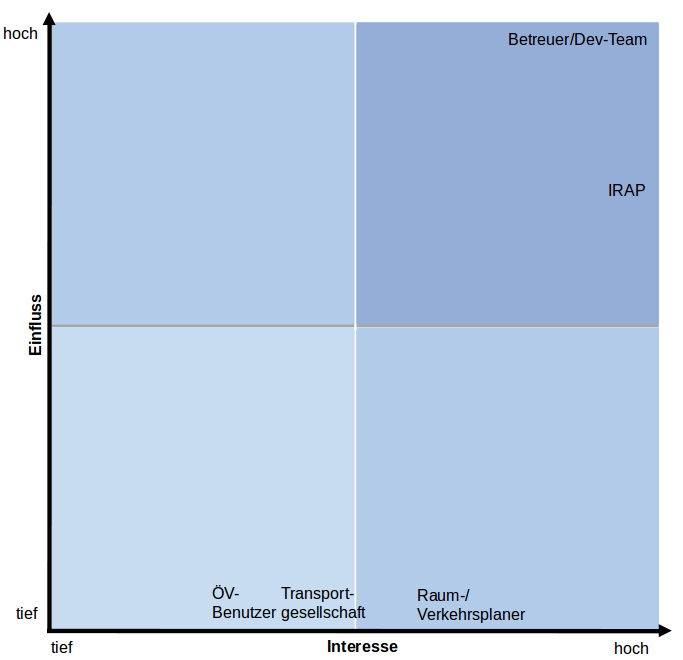
\includegraphics[width=0.7\linewidth]{projectdoc/img/stakeholder_map}
\caption[Stakeholder Map]{Stakeholder Map}
\label{fig:stakeholder_map}
\end{figure}



\begin{landscape}
\begin{longtable}{l p{9cm} p{9cm}}
        \toprule
        \textbf{Stakeholder}
                                & \textbf{Interesse}
                                & \textbf{Einfluss} \\
        \midrule
        \textbf{Betreuer (Prof. Stefan Keller)}
                                & Erfolgreiche Bachelorarbeit, welche Themengebiete des Geometa Lab tangiert und nach Abschluss einen konkreten Nutzen erbringt.
                                & Einfluss auf die Definition der Aufgabenstellung, Anforderungen, Rahmenbedingungen, laufende Steuerung des Projekts in enger Zusammenarbeit mit dem Dev-Team. \\
        \textbf{Dev-Team}
                                & Erfolgreiche Bachelorarbeit, in welcher das erlernte Wissen des Studiums konkret angewendet werden kann und das Thema „Netzwerkanalyse“ im OSM-Umfeld aufgreift. Die BA soll ein Produkt hervorbringen, welches von unterschiedlichen Personengruppen eingesetzt werden kann.
                                & Einfluss auf die Definition der Aufgabenstellung, Anforderungen,  Rahmenbedingungen, laufende Steuerung des Projekts in enger Zusammenarbeit mit dem Betreuer. \\                                
        \textbf{IRAP (Prof. Claudio Büchel)}
                                & Interessen analog zu Raumplaner/Verkehrsplaner. Durch die praktische Erfahrung mit der bisherigen Norm existiert ein aktives Interesse, diese neu zu gestalten und für die Zukunft fit zu machen.
                                & Nimmt die \gls{OeVGK18}-Spezifikation ab und gestaltet die Spezifikation aktiv mit. \\
        \textbf{Raumplaner/Verkehrsplaner}
                                & Gemäss Verordnung werden nur noch Gebiete mit einer guten ÖV-Erschliessung verdichtet. Mit den Güteklassen lässt sich prüfen, an welchen Standorten eine Verdichtung stattfinden kann.
                                & Hat keinen direkten Einfluss. Die Interessen fliessen in die Anforderungen. \\     
        \textbf{Transportgesellschaften}
                                & Transportgesellschaften überprüfen mit den Güteklassen die aktuelle Erschliessung der Schweiz und können dadurch Erweiterungspotential eruieren.
                                & Hat keinen direkten Einfluss. Die Interessen fliessen in die Anforderungen. \\       
        \textbf{Dev-Team}
                                & ÖV-Benutzer, welcher auf der Wohnungssuche ist, prüft mit den Güteklassen die Erschliessung eines potentiellen Wohnortes.
                                & Hat keinen direkten Einfluss. Die Interessen fliessen in die Anforderungen. \\                                                   
        \bottomrule
    \caption{Stakeholder}
    \label{table:Stakeholder}
\end{longtable}
\end{landscape}

\subsection{Risiken}
\label{Projektmanagement:Risiken}

\begin{longtable}{p{0.5cm} p{7cm} p{2cm} p{2cm} p{2cm}}
    \toprule
      \textbf{ID}
    & \textbf{Risiko}
    & \textbf{max. Schaden [h]}
    & \textbf{WSK}
    & \textbf{gewichteter Schaden} \\
    \midrule
    \textbf{1}
                    & Definition der \gls{OeVGK18}-Spezifikation findet kein Ende.
                    & 20
                    & 30%
                    & 6 \\
    \textbf{2}
                    & PostGIS und pgRouting eignet sich nicht für die \acs{ÖV}-Güteklasse-Berechnung.
                    & 40
                    & 25%
                    & 10 \\
    \textbf{3}
                    & PostGIS und pgRouting sind technologisches Neuland.
                    & 24
                    & 30%
                    & 7.2 \\
    \textbf{4}
                    & Es existieren viele Abhängigkeiten auf Fremdsysteme.
                    & 8
                    & 20%
                    & 1.6 \\
    \textbf{5}
                    & Fremdsysteme bieten nicht die geforderte Datenqualität.
                    & 24
                    & 20%
                    & 4.8 \\
    \textbf{6}
                    & Frontend-Framework eignet sich nicht für Karten-Integration.
                    & 16
                    & 30%
                    & 4.8 \\
    \bottomrule
    \caption{Risiken}
    \label{table:Risiken}
\end{longtable}

In der Tabelle \ref{table:Risiken} sind die identifizierten Projektrisiken aufgelistet.
Grundsätzlich lässt sich sagen, dass sich alle Risiken in einem vertretbaren Rahmen befinden.
Das Hauptrisiko der Bachelorarbeit ist das technische Neuland und die fehlende Erfahrung mit PostGIS und pgRouting.
Der Umgang und die Konsequenzen, welche sich aus der Risikoanalyse ableiten, sind in den folgenden Unterkapitel beschrieben.
Die Risiken werden in einem zwei-wöchentlichen Rhythmus diskutiert und bei Unstimmigkeiten revidiert und neue Massnahmen getroffen.

\begin{figure}[ht]
    \centering
    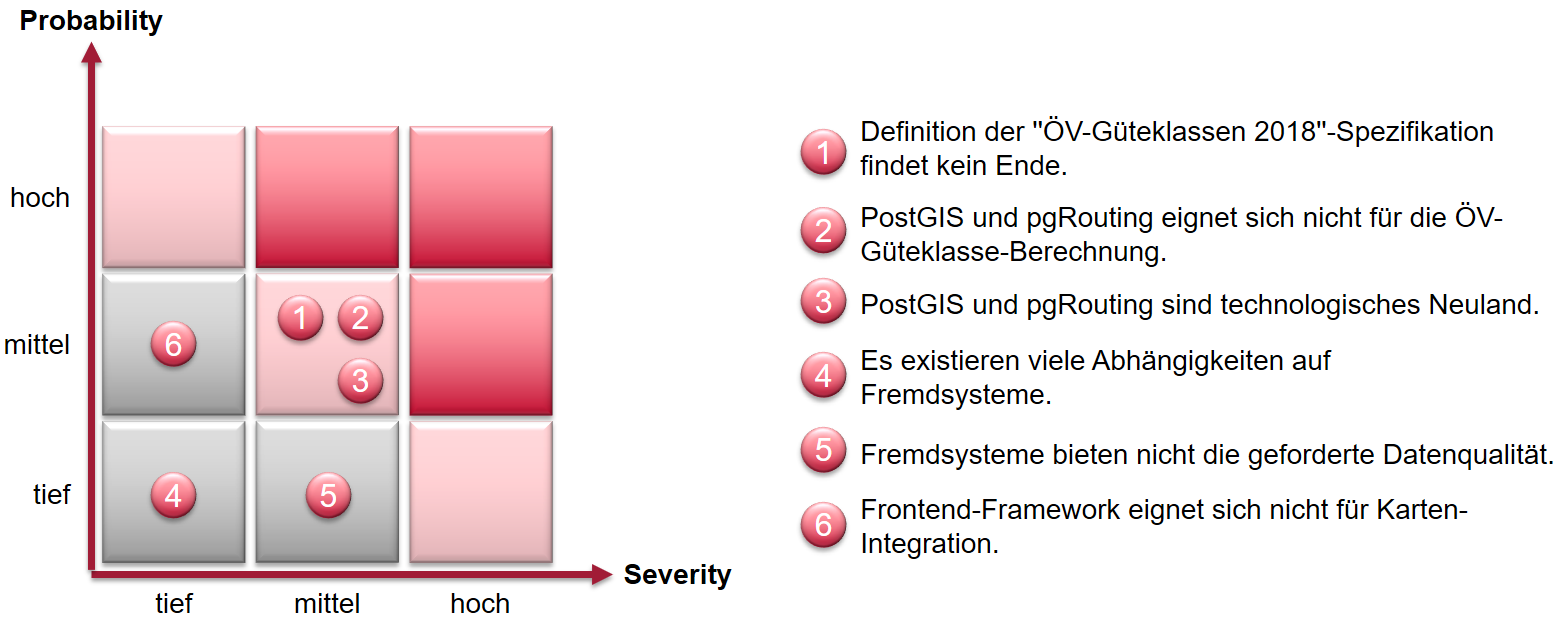
\includegraphics[width=1.0\linewidth]{projectdoc/img/risk_analysis}
    \caption[Risiko-Analyse]{Risiko-Analyse}
    \label{fig:risk_analysis}
\end{figure}

\subsubsection{Umgang mit Risiken}
\label{Risiken:Umang mit Risiken}

Die Risikoanalyse hat einen erwarteten Mehraufwand von \emph{34.4} Stunden ergeben.
Den in Tabelle \ref{table:Risiken} identifizierten technischen Risiken (\emph{ID 2, 3 und 6}) wird mit einer geplanten Einarbeitung und Prototypen entgegen gewirkt.
Damit die Spezifikation der \gls{OeVGK18} ein definitives Ende findet und mit der Umsetzung begonnen werden kann, wird ein fixer Milestone "`Spezifikation umsetzungsbereit"' definiert, welcher zwei Überarbeitungsrunden beinhaltet.

\subsubsection{Konsequenz}
\label{Risiken:Konsequenz}

Falls die geplanten Massnahmen nicht den erwarteten Nutzen zeigen oder unerwartete Stolpersteine auftreten, wird der Use Case \nameref{Use Cases:UC05} aus dem Scope gestrichen.

\subsubsection{Risiko-Refinement}
\label{Risiken:Risiko-Refinement}

Alle zwei Wochen findet ein Risiko-Refinement statt.
Zweck dieses Meeting ist es, dass die Risiken mit der aktuellen Situation abgeglichen werden.
Bei Bedarf kann so rasch auf eintretende Risiken reagiert und mit den betroffenen Stakeholder einen Konsens über das weitere Vorgehen gefunden werden.



\section{Softwaredokumentation}
\label{Softwaredokumentation}

In diesem Kapitel wird die Bedienung der Software beschrieben.
Diese besteht aus dem \nameref{Implementation:ÖV-Güteklassen 2018 Generator}, dem Backend und dem Frontend.

Mit dem Generator werden zuerst die \ac{ÖV}-Güteklassen erzeugt.
Mit dem Resultat davon wird das Backend, ein HTTP-Server, gestartet.
Dieser wiederum wird vom Frontend als Datenquelle gebraucht, um die \acs{ÖV}-Güteklassen zu visualisieren.

\subsection{ÖV-Güteklassen 2018 Generator}
\label{Softwaredokumentation: ÖV-Güteklassen 2018 Generator}

\subsubsection{Vorbereitung}
\label{Softwaredokumentation:Vorbereitung}
Als Vorbereitung für das Generieren der \ac{ÖV}-Güteklassen wird eine Datenbank aufgesetzt, die alle zur Berechnung nötigen Daten, Schemas und Indices enthält.
Um diesen Prozess möglichst automatisiert und reproduzierbar auszuführen, wurden entsprechende Docker-Container und Scripts vorbereitet.
Vorgängig müssen dazu die Terraindaten der Schweiz als TIF besorgt werden.
% TODO werden OSM-Daten zum Schluss auch automatisch herunter geladen?
Die restlichen Daten werden werden automatisch während dem Setup vom Internet bezogen.

Die genaue Anleitung zur Vorbereitung der Datenbank ist auf Github~\cite{github_docker_setup} verfügbar.




% not included in released version
% \chapter{Anhänge}


\section{Persönliche Berichte}
\label{Persönliche Berichte}

\subsection{Robin Suter}
\label{Persönliche Berichte:Robin Suter}

Während ich mit der Studienarbeit im letzten Semester erste Erfahrungen mit Geodaten und insbesondere \gls{OpenStreetMap} machen konnte, bot mir diese Arbeit eine gute Gelegenheit, diese Kenntnisse zu vertiefen und sie auf eine neue Problemdomäne anzuwenden.
Spannend war insbesondere die Verbindung von Geodaten und Verkehrsplanung.
Das Erarbeiten der Spezifikation hat mir einen guten Einblick in dieses Gebiet verschafft.

Aus der technischen Perspektive fand ich vor allem die Arbeit mit PostgreSQL beziehungsweise PostGIS sehr interessant.
Ich konnte ein vertieftes Verständnis von SQL erlangen und lernte viel über die Optimierung von SQL-Queries.

Die Arbeit im Team mit Jonas Matter ist sehr gut gelungen.
Es gab viele Momente, an denen wir mit gemeinsamen Austausch von Ideen rasch zu neuen Lösungsmöglichkeiten gelangten.
Auch unser Prozess der gegenseitigen Reviews hat uns geholfen, die Qualität kontinuierlich hoch zu halten.

Insgesamt bin ich mit dem Verlauf und dem Ausgang dieser Bachelorarbeit sehr zufrieden.
Wir haben alle Ziele erreicht, die wir zu Beginn ausgelegt haben und die Zeitplanung ist zum Ende hin optimal aufgegangen.
Ich hoffe auch, dass unsere erarbeitete Spezifikation auf Interesse stösst und in Zukunft weiter entwickelt wird.

\subsection{Jonas Matter}
\label{Persönliche Berichte:Jonas Matter}

Die branchenübergreifende Arbeit hat mein Interesse von Anfang an geweckt.
Die Verbindung von grossen Mengen an Daten, dessen Verarbeitung und der Einsatz von PostGIS und pgRouting versprach eine gute Kombination.
Grosse Freude haben mir die verschiedenen Optimierungen, welche der Generator durchlebt hat, bereitet.

Die Zusammenarbeit mit Robin Suter war wie in vorherigen Projekten optimal.
Die regelmässigen Reviews sowie Pair Programming haben zu einer stetigen Steigerung der Qualität geführt.
Durch Hinterfragen der gegenseitigen Lösungen wurde man auf neue Wege geführt, welche man in Einzeilarbeit nicht eingeschlagen hätte.

Abschliessend kann ich sagen, dass ich mit dem Verlauf und dem Resultat der Bachelorarbeit sehr zufrieden bin.
Ich hoffe, dass die ÖV-Güteklassen 2018 bei den unterschiedlichen Stakeholdern Anklang finden wird, sei dies durch die Verwendung der Web-App und des Generators oder der Weiterverwendung und Verbesserung der Spezifikation.

\section{Projektmonitoring}
\label{sec:Projektmonitoring}

\subsection{Auswertung Velocity}
\label{sub:Auswertung Velocity}

\begin{figure}[H]
    \centering
    \begin{tikzpicture}
        \begin{axis}[
            ybar,
            width=0.85\textwidth,
            bar width=5pt,
            ylabel={Sprint Velocity},
            xlabel={Sprint Nr.},
            ymin=0,
            ymax=80,
            xtick=data
        ]
            \addplot[style={blue, fill=blue!30!white}] coordinates
                {(1, 44.5) (2, 40.5) (3, 30.5) (4, 29) (5, 34) (6, 42) (7, 37)
                (8, 39) (9, 41) (10, 39) (11, 35) (12, 24) (13, 39) (14, 38.5) (15, 63.5) (16, 61.5)};
            \addplot [style={red, fill=red!30!white}] coordinates
                {(1, 40.5) (2, 36.5) (3, 18.5) (4, 25) (5, 32) (6, 38) (7, 37)
                (8, 39) (9, 41) (10, 28.5) (11, 35) (12, 36) (13, 36) (14, 38.5) (15, 68.5) (16, 61.5)};
            \legend{Story-Points geplant,Story-Points erledigt}
        \end{axis}
    \end{tikzpicture}%

    \caption[Diagramm Velocity über das Projekt]{Sprint Velocity über den Verlauf des Projekts}
    \label{chart:sprint_velocity}
\end{figure}

Im Diagramm \ref{chart:sprint_velocity} ist die Sprint Velocity für jeden Sprint über den Verlauf des Projekts aufgezeichnet.
Ein Sprint dauerte jeweils eine Woche.
Zu Beginn haben wir 40 Story-Points geplant, bei jedem weiteren Sprint haben wir uns am vorherigen Sprint orientiert, wie viele Story-Points wir planen.

Ganz zu Beginn funktionierten die 40 Story-Points noch gut, aber bei Sprints 3 gab es einen Einbruch, weil wir Arbeitspakete zu gross geschätzt haben.
Dadurch wurden sie nicht innerhalb einer Woche fertig.
In den nachfolgenden Sprints konnten wir uns korrigieren und wieder auf ca. 40 Story-Points einpendeln.
Ab Sprint 12 gab es einige Einbrüche, weil andere Module gegen Ende des Semesters viel Zeit beanspruchten.
In den letzten zwei Wochen haben wir deutlich mehr Story-Points eingeplant, da das reguläre Semester vorbei war und wir uns voll auf diese Arbeit fokussieren konnten.

\subsection{Zeitauswertung}
\label{sub:Zeitauswertung}

\begin{figure}[H]
    \centering
    \begin{tikzpicture}
        \begin{axis}[
            ybar,
            width=0.85\textwidth,
            bar width=10pt,
            ylabel={Geleistete Arbeitsstunden},
            xlabel={Woche},
            ymin=0,
            ymax=100,
            xtick=data,
            nodes near coords,
            nodes near coords align={vertical},
            every node near coord/.append style={color=black, font=\small}
        ]
            \addplot[style={orange, fill=orange!30!white}] coordinates
                {(1, 30.2) (2, 23.7) (3, 35.3) (4, 36.9) (5, 37.9) (6, 47.5) (7, 49.3)
                (8, 38) (9, 37.8) (10, 24) (11, 51.4) (12, 51.8) (13, 71.5) (14, 38.4) (15, 67.4) (16, 79.4)};
        \end{axis}
    \end{tikzpicture}

    \caption[Diagramm Zeitaufwand über den Verlauf des Projekts]{Zeitaufwand über den Verlauf des Projekts}
    \label{chart:Zeitauswertung_weeks}
\end{figure}

Im Diagramm \ref{chart:Zeitauswertung_weeks} sind die geleisteten Arbeitsstunden pro Woche aufgeschlüsselt.
Der Soll-Wert des gesamten Projekts ist 720 Arbeitsstunden.
Diese sind aufgeteilt auf ca. 37 Stunden / Woche während dem Semester und 80 Stunden / Woche für die letzten zwei Wochen nach Semesterende.

In den ersten Wochen wurde weniger Arbeit als das Soll geleistet, in der Mitte konnte diese Zeit aber aufgeholt werden.
Zwischendurch gab es unregelmässige Einbrüche.
Diese sind darauf zurück zu führen, dass in diesen Wochen viel Aufwand für andere Module entstanden ist.

Insgesamt wurden bis 3 Tage vor Abschluss \textbf{730 Arbeitsstunden} geleistet.
Die Arbeitsstunden pro Person sind mit \textbf{363 h} (Jonas Matter) und \textbf{367 h} (Robin Suter) sehr ähnlich verteilt.


\begin{figure}[H]
    \centering
    \begin{tikzpicture}
        [
            pie chart,
            slice type={admin}{piered},
            slice type={analysis}{pieyellow},
            slice type={backend}{pielblue},
            slice type={generator}{pieblue},
            slice type={infrastruktur}{pielgreen},
            slice type={thesis}{piegreen},
            slice type={webapp}{piecyan},
            slice type={specification}{piebrown},
            pie values/.style={font={\small}},
            scale=3
        ]

            \pie[xshift=2cm]{Arbeitsstunden pro Komponente}{32/generator,28/thesis,12/admin,9/webapp,6/analysis,5/specification,5/backend,3/infrastruktur}

            \legend[shift={(0cm,-1cm)}]{{OeVGK18-Generator}/generator, {Thesis}/thesis, {Administration}/admin, {Web-Applikation}/webapp}
            \legend[shift={(3cm,-1cm)}]{{Analyse}/analysis, {OeVGK18-Spezifikation}/specification, {Backend}/backend, {Infrastruktur}/infrastruktur}

        \end{tikzpicture}

    \caption[Diagramm Zeitaufwand pro Komponente]{Zeitaufwand verteilt auf einzelne Komponenten}
    \label{chart:Zeitauswertung_components}
\end{figure}

Im Diagramm \ref{chart:Zeitauswertung_components} sind die total geleisteten Arbeitsstunden auf einzelne Komponenten aufgeteilt.
Wie zu sehen ist, wurde für die Implementation des ÖV-Güteklassen 2018 Generators und das Schreiben der Arbeit jeweils rund ein Drittel der Zeit aufgewendet.
\cleardoublepage
\addcontentsline{toc}{section}{Formulare}
\includepdf[frame, scale=.9]{additionals/eigenstaendigkeitserklaerung.pdf}
\includepdf[frame, scale=.9]{additionals/vereinbarung_nutzungsrechte.pdf}

\printglossary[type=main,title=Glossar]

% \ac prints the longform the first time, after that the short
% using \acs always prints the shortform
   
\chapter*{Abkürzungsverzeichnis}\addcontentsline{toc}{chapter}{Abkürzungsverzeichnis}
\begin{acronym}[REST] % [] should contain the longest acronym
    \acro{OSM}{OpenStreetMap}
    \acro{RUP}{Rational Unified Process}
    \acro{API}{Application Programming Interface}
    \acro{UML}{Unified Modeling Language}
    \acro{REST}{Representational state transfer}
    \acro{CI}{Continuous Integration}
    \acro{TDD}{Test-Driven Development}
    \acro{ARE}{Bundesamt für Raumentwicklung}
\end{acronym}


\nocite{*}
\cleardoublepage % https://tex.stackexchange.com/a/98995
\phantomsection
\addcontentsline{toc}{chapter}{Literaturverzeichnis}
\bibliographystyle{IEEEtran}
\bibliography{thesis}

\cleardoublepage
\phantomsection
\addcontentsline{toc}{chapter}{Abbildungsverzeichnis}
\listoffigures

\cleardoublepage
\phantomsection
\addcontentsline{toc}{chapter}{Tabellenverzeichnis}
\listoftables

\renewcommand\listoflistingscaption{Code Listings}
\listoflistings
\addcontentsline{toc}{chapter}{Code Listings}

\end{document}
